\documentclass[11pt,a4paper]{article}
% a minimum font size of 11 points, except for the Gantt chart and tables where the minimum font size is 8 points
%8 points for 11pt is \scriptsize
\usepackage{lipsum}
\usepackage[gen]{eurosym}
\usepackage{framed}
\usepackage{layout}
\usepackage{layouts}
\usepackage{caption}
\usepackage{placeins}
\usepackage{lastpage}
\usepackage{color}
\usepackage[pdftex]{epsfig}
\DeclareGraphicsExtensions{.jpg,.mps,.pdf,.png,.eps}
\usepackage{graphicx}
\usepackage{graphics}
\usepackage{pdfpages}
\usepackage{amssymb,amsmath, multicol, latexsym,mathrsfs,multirow}
\usepackage{xspace}
\usepackage{wrapfig}
\usepackage{comment}
\usepackage{fancyhdr}
\usepackage{titlesec}
\usepackage{titling}
%automate spacesaving
\usepackage[lists=tight, title=tight, sections=tight, margins=normal, wordspacing=tight, paragraphs=tight, tracking=tight, charwidths=tight]{savetrees} %wordspacing=normal, 
% Uncomment here if you want to go back to manual spacesaving
%\usepackage{enumitem}
\usepackage{rotating}
\usepackage[absolute,overlay]{textpos}
\usepackage{framed}
\usepackage{colortbl,ctable,hhline}
\usepackage{pbox}
\usepackage{footnote}
\usepackage[para]{footmisc}
\usepackage{tablefootnote}
\usepackage[nomarkers,nolists]{endfloat}
%\usepackage[float]
%\restylefloat{figure}

\makesavenoteenv{tabular}
%\makesavenoteenv{table}

\usepackage{chngcntr}
\counterwithin{table}{subsection}
\usepackage{longtable}

\usepackage[italic]{hepparticles}
\usepackage[italic]{hepnames}
\usepackage[pdftex,unicode]{hyperref}

%correlct umlauts
\usepackage[utf8]{inputenc}

%\usepackage{cite}
%\usepackage[numbers,sort&compress]{natbib}
%\usepackage{hypernat}%,natbibspacing}
%\bibliographystyle{mybib/short_style_m}

\setlength{\columnseprule}{.4pt} 

%\usepackage[colorgrid,texcoord]{eso-pic}\TPshowboxestrue  

%bibliography
% Taken from https://github.com/sean-chester/H2020-MSCA-IF-2016/blob/master/IF-2016-Part_B.tex
\usepackage[style=verbose-ibid,backend=biber]{biblatex}

% vertical page and text spacing
\topmargin -11mm
\headheight 14pt
\headsep 2.5mm
\footskip 6.5mm
\textheight 240mm
%\parskip 3pt
\def\baselinestretch{1.}

% horizontal page spacing
\oddsidemargin -10.5mm
\textwidth  180mm

%fonts
% Palatino for main text and math
%\usepackage[osf,sc]{mathpazo}

%\usepackage{utopia}

%Garamond saves space and looks way poncier
\usepackage[T1]{fontenc}
\usepackage[urw-garamond]{mathdesign}
%\usepackage{ebgaramond}
\renewcommand\labelitemi{$\bullet$}

% Helvetica for sans serif
% (scaled to match size of Palatino)
\usepackage[scaled=0.90]{helvet}

% Bera Mono for monospaced
% (scaled to match size of Palatino)
\usepackage[scaled=0.85]{beramono}

% title and spacing
%\newfontfamily\headingfont[]{Palatino}
\titleformat{\section}{\Large\fontseries{b}\color{blue}}{B\thesection.}{1em}{}
\titleformat{\subsection}{\large\fontseries{b}\color{blue}}{B\thesubsection}{1em}{}
\titleformat{\subsubsection}{\fontseries{b}\color{blue}}{B\thesubsubsection}{1em}{}
\titlespacing*{\section}{0pt}{*2}{*1}
\titlespacing*{\subsection}{0pt}{*2}{*.75}
\titlespacing*{\subsubsection}{0pt}{*2}{*.75}
%bibliography
\renewcommand{\footnotesize}{\fontsize{8bp}{1em}\selectfont}
\renewcommand{\cite}{\autocite} % citations in footnotes
\addbibresource{SMARTHEP17_main.bib}
% Explicitly set footnote font size to match call (i.e., 8pt).
% Taken from http://tex.stackexchange.com/a/249422/84485
\makeatletter
\renewcommand\footnotesize{%
   \@setfontsize\footnotesize\@ixpt{8}%
   \abovedisplayskip 8\p@ \@plus2\p@ \@minus4\p@
   \abovedisplayshortskip \z@ \@plus\p@
   \belowdisplayshortskip 4\p@ \@plus2\p@ \@minus2\p@
   \def\@listi{\leftmargin\leftmargini
               \topsep 4\p@ \@plus2\p@ \@minus2\p@
               \parsep 2\p@ \@plus\p@ \@minus\p@
               \itemsep \parsep}%
   \belowdisplayskip \abovedisplayskip
}
\renewcommand\tableofcontents{%
    \@starttoc{toc}%
}
\makeatother

%float spacing
\setlength{\textfloatsep}{9pt plus 2.0pt minus 4.0pt}
\setlength{\floatsep}    {8pt plus 2.0pt minus 4.0pt}
\setlength{\intextsep}   {9pt plus 2.0pt minus 4.0pt}

%start title page
\def\acronym{SMARTHEP\xspace}
\newcommand{\ShortDescriptionWPOne}{Real-time data analysis}
\newcommand{\ShortDescriptionWPTwo}{Deep learning and multivariate analysis}
\newcommand{\ShortDescriptionWPThree}{New figures of merit and developments}
\newcommand{\ShortDescriptionWPFour}{Detector development and optimization}

\pagestyle{fancy}
\lhead{}
\chead{\textbf{ \acronym\ -\ ETN}}
\rhead{}
\lfoot{}
\cfoot{\textbf{Part B\ -\ Page \thepage}}%\ of \pageref{LastPage}}}
\rfoot{}
\renewcommand{\headrulewidth}{0pt}
\renewcommand{\footrulewidth}{0pt}


\message{YYY \the\footskip}

%\newcommand{\vs}{\vspace{-0.3cm}}
\newcommand{\ite}[1]{\vspace{-0.25cm}\item[\mbox{[#1]}]}
\newcommand{\iteCV}{\vspace{-0.25cm}\item[$\circ$]}

\captionsetup[table]{position=above,skip=-12pt,singlelinecheck=false}
\captionsetup{font=footnotesize}

\hypersetup{ a4paper
            ,pdfauthor={Johannes Albrecht, Caterina Doglioni, Vladimir Gligorov}
            ,pdfview={FitV}
            ,pdfstartview={FitV}
            %,pdfborder={0000}
            %,pdfborder= {255 0 0}
            ,pdfborderstyle={/S/U/W 1}
            ,urlbordercolor = red
            ,citebordercolor = white
            ,linkbordercolor = white
	        }

%%%%%%%%%%%%%%%%%%%%%%%%%%%%%
%%%  Definitions definitions
%%%%%%%%%%%%%%%%%%%%%%%%%%%%%


\newcommand{\cp}{\mcal{CP}\xspace}
\newcommand{\NP}{New Physics\xspace}

\newcommand{\pT}{\ensuremath{p_{\rm T}}\xspace}
\newcommand{\ET}{\ensuremath{E_{\rm T}}\xspace}
\newcommand{\IP}{\ensuremath{{\rm IP}}\xspace}
\newcommand{\IPS}{\ensuremath{{\rm IPS}}\xspace}
\newcommand{\DOF}{\ensuremath{{\rm DOF}}\xspace}
\newcommand{\DOFS}{\ensuremath{{\rm DOFS}}\xspace}
\newcommand{\DOCA}{\ensuremath{{\rm DOCA}}\xspace}
\newcommand{\GL}{\ensuremath{{\rm GL}}\xspace}
\newcommand{\signif}[1]{\ensuremath{\rm #1\!/\!\sigma_{#1}}}
\newcommand{\signifm}[1]{\ensuremath{#1\!/\!\sigma_{#1}}}
\newcommand{\sig}[1]{\ensuremath{\frac{#1}{\sigma_{#1}}}\xspace}
\newcommand{\DLL}[2]{\ensuremath{\rm \Delta  \ln{\cal L}_{\particle{#1}\particle{#2}}}}
\newcommand{\Dll}[2]{\ensuremath{\Delta\textrm{LL}_{\particle{#1}\particle{#2}}}}
\newcommand{\BR}[1]{\ensuremath{\mathcal{B}(#1)}\xspace}
\newcommand{\BF} {branching fraction\xspace}
\newcommand{\BFs}{branching fractions\xspace}
\newcommand{\Cer}{\v Cerenkov\xspace}
\newcommand{\cer}{\v cerenkov\xspace}
\newcommand{\we}{\ensuremath{\theta_{\rm W}}\xspace}
\def\idmath{\mbox{l\hspace{-0.5em}1} }
\def\idmath2{\mbox{\scriptsize l\hspace{-0.5em}1 }}


\newlength{\MarcoH}  %%  http://www.tac.dk/cgi-bin/info2www?(latex)Lengths
\newlength{\MarcoL}
\newcommand{\TwoUp}[1]{
\settoheight{\MarcoH}{#1}
\settowidth{\MarcoL}{#1}
\raisebox{0.5\MarcoH}{#1}\hspace{-\MarcoL}\raisebox{-0.5\MarcoH}{#1}}


\newcommand{\sm}{SM\xspace}
\newcommand{\CL}{C.L.\xspace}
\newcommand{\ie}{\textit{i.e.}\xspace}
\newcommand{\eg}{\textit{e.g.}\xspace}
\newcommand{\wrt}{w\!.r\!.t.\xspace}
\newcommand{\etal}{\textit{et al.}\xspace}
\newcommand{\belle}{Belle\xspace}
\newcommand{\babar}{{\sc BaBar}\xspace}
\newcommand{\teva}{Tevatron\xspace}
\newcommand{\tbe}{\ensuremath{\tan \beta}\xspace}
\newcommand{\mcal}[1]{\ensuremath{\mathcal{#1}}\xspace}
\newcommand{\phd}{Ph.\@{}D.\@{}\xspace}

\newcommand{\IT}{Inner Tracker\xspace}
\newcommand{\vel}{VeLo\xspace}
\newcommand{\vs}{\textit{vs}\xspace}
\newcommand{\MC}{Monte Carlo\xspace}

\newcommand{\qsq}{{\ensuremath{q^2}}\xspace}
\newcommand{\fl}{\ensuremath{F_{\textrm{L}}}\xspace}
\newcommand{\afb}{\ensuremath{A_{\textrm{FB}}}\xspace}
\newcommand{\at}[1]{\ensuremath{A_{T}^{(#1)}}\xspace}



%%%%%%%%%%%%%%%%%%%%%%%%%%%
%%%         Particles
%%%%%%%%%%%%%%%%%%%%%%%%%%%

\newcommand{\BAR}[1]{\overline{#1}}
\newcommand{\particle}[1]{{\ensuremath{ #1}}\xspace}


\newcommand{\pp}{\particle{pp}}
\newcommand{\ppbar}{\particle{p\BAR{p}}}
\newcommand{\cc}{\particle{c\BAR{c}}}
\renewcommand{\b}{\particle{b}}
\newcommand{\bbar}{\particle{\BAR{b}}}
\newcommand{\bb}{\particle{b\BAR{b}}}


%Bees
\newcommand{\B}{\PB}
\newcommand{\Bs}{\PBs}
%\newcommand{\Bsd}{\particle{B^0_{(s,d)}}}
\newcommand{\Bd}{\PBzero}
\newcommand{\Bds}{\HepParticle{B}{(s)}{0}\xspace}
\newcommand{\Bu}{\PBplus}
\newcommand{\Bc}{\PBc}
\newcommand{\Lb}{\PLambdab}
\newcommand{\Bbar}{\APB}
\newcommand{\Bsbar}{\APBs}
\newcommand{\Bdbar}{\APBzero}
\newcommand{\Bdsbar}{\HepAntiParticle{B}{(s)}{0}}
\newcommand{\Bubar}{\PBminus}
\newcommand{\Bcbar}{\APBc}
\newcommand{\Lbbar}{\HepAntiParticle{\Lambda}{b}{}}

\newcommand{\Ks}{\PKs}
\newcommand{\Ko}{\PKzero}
\newcommand{\Kl}{\PKl}
\newcommand{\Kp}{\PKplus}
\newcommand{\Km}{\PKminus}
\newcommand{\Kst}{\HepParticle{K}{}{\ast0}}
\newcommand{\APKst}{\HepAntiParticle{K}{}{\ast0}}
\newcommand{\Jpsi}{\PJpsi}
\newcommand{\Jmm}{\PJpsi(\Pgm\Pgm)}
\newcommand{\mup}{\Pgmp}
\newcommand{\mum}{\Pgmm}

\newcommand{\Dp}{\PDplus}
\newcommand{\Dm}{\PDmimus}
\newcommand{\Do}{\PDzero}
\newcommand{\Dob}{\APDzero}
\newcommand{\Dst}{\PDstar}
\newcommand{\Dsto}{\HepParticle{D}{}{\ast0}} 
\newcommand{\Dstob}{\HepAntiParticle{D}{}{\ast0}} 
\newcommand{\Dstb}{\HepAntiParticle{D}{}{\ast}} 
\newcommand{\Dstp}{\HepParticle{D}{}{\ast+}}
\newcommand{\Dstm}{\HepParticle{D}{}{\ast-}}
\newcommand{\DDst}{\HepParticle{DD}{}{\ast}}

\newcommand{\pio}{\Ppizero}
\newcommand{\pip}{\Ppiplus}
\newcommand{\pim}{\Ppiminus}

% kaons
\newcommand{\Fii}  {\particle{f_2^{\prime}}(1525)}
\newcommand{\Kii}  {\particle{K_2^{\ast0}}(1430)}
\newcommand{\Kiii} {\particle{K_1}(1270)}
\newcommand{\Kiiii}{\particle{K_1}(1400)}


\DeclareRobustCommand{\PUpsilonFiveS}{\HepParticleResonance{\PgU}{5S}{}{}\xspace}
\DeclareRobustCommand{\Phplus} {\HepParticle{h}{}{+}\xspace}
\DeclareRobustCommand{\Phminus}{\HepParticle{h}{}{-}\xspace}

\DeclareRobustCommand{\PJpsi}{\HepParticle{J\!/\!\psi}{}{}\xspace}

%Decays
\newcommand{\decay}[2]{\particle{#1\!\to #2}}

\newcommand{\bsgamma}{\decay{b}{s \gamma}}
\newcommand{\bsll}{\decay{b}{s \ell \ell}}
\newcommand{\Bsmumu}{\decay{\Bs}{\mup\mum}}
\newcommand{\Bdmumu}{\decay{\Bd}{\mup\mum}}
\newcommand{\Bdsmumu}{\decay{\Bds}{\mup\mum}}
\newcommand{\Bsbarmumu}{\decay{\Bsbar}{\mup\mum}}
\newcommand{\Bsmumugamma}{\decay{\Bs}{\mup\mum\Pphoton}}
\newcommand{\Bdpipi}{\decay{\Bd}{\pip\pim}}
\newcommand{\BsKK}{\decay{\Bs}{ \PKplus \PKminus}}
\newcommand{\BdKpi}{\decay{\Bd}{ \PKplus\pim}}
\newcommand{\BspiK}{\decay{\Bs}{\pip \PKminus}}
\newcommand{\Bhh}{\decay{\Bds}{ \Phplus\Phminus}}
\newcommand{\Buhhh}{\decay{\PBpm}{ \Phplus \Phminus h^{\pm}}}
\newcommand{\BsDspi}{\decay{\Bs}{\PDsminus \pip}}
\newcommand{\BsJpsiPhi}{\decay{\Bs}{\PJpsi \Pphi}}

\newcommand{\BuJpsiK}{\decay{\PBplus}{\PJpsi \PKplus}}
\newcommand{\BuJPsiK}{\decay{\PBplus}{\PJpsi \PKplus}}
\newcommand{\BuJpsimumuK}{\decay{\PBplus}{\Jmm \PKplus}}
\newcommand{\BdJpsiKst}{\decay{\Bd}{\PJpsi \Kst}}
\newcommand{\BdJpsimumuKstKpi}{\decay{\Bd}{\Jmm \Kst(\Kp\pim)}}
\newcommand{\BcJpsimumumunu}{\decay{\PBc}{\Jmm\mup\Pnum}}
\newcommand{\Jpsimumu}{\decay{\PJpsi}{\mup\mum}}
\newcommand{\Lambdappi}{\decay{\PLambda}{\Pproton\pim}}

\newcommand{\BsPhimm}  {\decay{\PBs}{\Pphi\mup\mum}}
\newcommand{\BsPhiKKmm}{\decay{\PBs}{\Pphi(\to\PK\PK)\mup\mum}}
\newcommand{\BsFtwomm} {\decay{\PBs}{\Fii\mup\mum}}

\newcommand{\BdKstmm} {\decay{\Bd}{\Kst\mup\mum}}
\newcommand{\BdKstee} {\decay{\Bd}{\Kst e e}}
\newcommand{\BdKTwomm}{\decay{\PBd}{\Kii\mup\mum}}
\newcommand{\BdKOnemm}{\decay{\PBd}{\Kiii\mup\mum}}



%%%%%%%%%%%%%%%%%%%%%%%%%%%%%%%
%%% Units
%%%%%%%%%%%%%%%%%%%%%%%%%%%%%%%


\newcommand{\unit}[1]{\ensuremath{\,{\rm #1}}\xspace}

\newcommand{\kev}{\unit{keV}}
\newcommand{\mev}{\unit{MeV}}
\newcommand{\gev}{\unit{GeV}}
\newcommand{\tev}{\unit{TeV}}
\newcommand{\kevc}{\unit{keV}}
\newcommand{\mevc}{\unit{MeV\!/\!\textit{c}}}
\newcommand{\gevc}{\unit{GeV\!/\!\textit{c}}}
\newcommand{\tevc}{\unit{TeV\!/\!\textit{c}}}
\newcommand{\kevcc}{\unit{keV\!/\!\textit{c}^2}}
\newcommand{\mevcc}{\unit{MeV\!/\!\textit{c}^2}}
\newcommand{\gevcc}{\unit{GeV\!/\!\textit{c}^2}}
\newcommand{\tevcc}{\unit{TeV\!/\!\textit{c}^2}}

\newcommand{\mb}{\unit{mb}}
\newcommand{\microb}{\unit{\mu b}}
\newcommand{\pb}{\unit{pb}}
\newcommand{\fb}{\unit{fb}}
\newcommand{\invpb}{\unit{pb^{-1}}}
\newcommand{\invfb}{\unit{fb^{-1}}}
\newcommand{\unitlum}{\unit{cm^{-2}\,s^{-1}}}

\newcommand{\cm}{\unit{cm}}
\newcommand{\mm}{\unit{mm}}
\newcommand{\m}{\unit{m}}
\newcommand{\ps}{\unit{ps}}
\newcommand{\invps}{\unit{ps^{-1}}}
\newcommand{\fs}{\unit{fs}}
\newcommand{\micron}{\unit{\mu m}}
\newcommand{\mrad}{\unit{mrad}}

\newcommand{\degree}{\ensuremath{^\circ}\xspace}
\newcommand{\degC}{\ensuremath{^{\circ}\,{\rm C}}\xspace}
\newcommand{\V}{\unit{V}}
\newcommand{\A}{\unit{A}}
\newcommand{\Hz}{\unit{Hz}}
\newcommand{\MHz}{\unit{MHz}}

\newcommand{\robust}{alternate\xspace}
\newcommand{\Robust}{Alternate\xspace}
\newcommand{\rob}{\robust}
\newcommand{\Rob}{\Robust}

\newcommand{\std}{standard\xspace}
\newcommand{\Std}{Standard\xspace}

\newcommand{\CLsb}{\ensuremath{\textrm{CL}_{\textrm{s+b}}}\xspace}
\newcommand{\CLs}{\ensuremath{\textrm{CL}_{\textrm{s}}}\xspace}
\newcommand{\CLb}{\ensuremath{\textrm{CL}_{\textrm{b}}}\xspace}

\newcommand{\pdf}{p.d.f.\@{}\xspace}
\newcommand{\pdfp}{p.d.f.}
\newcommand{\pdfs}{p.d.f.s\xspace}

\newcommand{\tl}{\ensuremath{\theta_{l}}\xspace}
\newcommand{\tk}{\ensuremath{\theta_{K^*}}\xspace}
\renewcommand{\initialsOne}{BK}
\renewcommand{\initialsTwo}{VG}
\renewcommand{\initialsThree}{JA}
\newcommand{\sqrtSeven}{$\sqrt{s} = 7\,\textrm{TeV}$\xspace}

\newcommand{\checkme}[1]{\textcolor{red}{\textbf{#1}}}
\newcommand{\task}[1]{\textbf{Task\,#1}\xspace}
\newcommand{\deli}[1]{\textbf{#1}\xspace}
\newcommand{\WP}[1]{\textbf{WP#1}\xspace}
\newcommand{\esr}[1]{ESR#1\xspace}

\newcommand{\saclaylong}{CNRS\xspace}
\newcommand{\saclay}{CNRS\xspace}
\newcommand{\cnrs}{CNRS\xspace}
%\newcommand{\cnrsentity}{CNRS\xspace}
\newcommand{\cnrsentity}{\textsc{Cnrs}\xspace}
\newcommand{\lund}{Lund University\xspace}
\newcommand{\lundlong}{Lund University\xspace}
\newcommand{\lundshort}{Lund\xspace}
%\newcommand{\lundentity}{ULUND\xspace}
\newcommand{\lundentity}{\textsc{Ulund}\xspace}
\newcommand{\heidelberg}{University of Heidelberg\xspace}
\newcommand{\heidelberglong}{University of Heidelberg\xspace}
\newcommand{\heidelbergshort}{Heidelberg\xspace}
\newcommand{\hd}{Kirchhoff Institute for Physics\xspace}
\newcommand{\hdshort}{KIP\xspace}
%\newcommand{\heidelbergentity}{UHEI\xspace}
\newcommand{\heidelbergentity}{\textsc{Uhei}\xspace}
\newcommand{\helsinkilong}{University of Helsinki\xspace}
\newcommand{\helsinki}{Helsinki\xspace}
\newcommand{\helsinkishort}{UH\xspace}
%\newcommand{\helsinkientity}{UH\xspace}
\newcommand{\helsinkientity}{\textsc{Uh}\xspace}
\newcommand{\unigelong}{Universit\'{e} de Gen\`{e}ve\xspace}
\newcommand{\unige}{UniGe\xspace}
\newcommand{\unigeshort}{UniGe\xspace}
%\newcommand{\unigeentity}{UNIGE\xspace}
\newcommand{\unigeentity}{\textsc{Unige}\xspace}
\newcommand{\parisvava}{CNRS \xspace}
%\newcommand{\parisU}{UPMC Paris \xspace}
%\newcommand{\parisULong}{Pierre-and-Marie-Curie University \xspace}
\newcommand{\parisU}{Sorbonne U. \xspace}
\newcommand{\parisUentity}{\textsc{Su}\xspace}
\newcommand{\sorbonnelong}{Sorbonne Universit\'{e} \xspace}
%\newcommand{\sorbonneentity}{SU \xspace}
\newcommand{\sorbonneentity}{\textsc{Su}\xspace}
\newcommand{\parisUlong}{Sorbonne University \xspace}
\newcommand{ \dortmundLong}{TU Dortmund University\xspace}
\newcommand{ \dortmundLongBroken}{TU Dortmund\\University\xspace}
\newcommand{ \dortmund}{Dortmund\xspace}
%\newcommand{ \dortmundentity}{TUDO\xspace}
\newcommand{ \dortmundentity}{\textsc{Tudo}\xspace}
\newcommand{ \nikheflong}{National Institute\\for Subatomic\\Physics, Nikhef\xspace}
\newcommand{ \nikhef}{Nikhef\xspace}
%\newcommand{ \nikhefentity}{Nikhef\xspace}
\newcommand{ \nikhefentity}{\textsc{Nikhef}\xspace}
\newcommand{ \radboudlong}{Radboud University, Nijmegen\xspace}
\newcommand{ \radboudlongbroken}{Radboud University, \\Nijmegen\xspace}
\newcommand{ \radboud}{Radboud University\xspace}
%\newcommand{ \radboudentity}{RU\xspace}
\newcommand{ \radboudentity}{\textsc{Ru}\xspace}
\newcommand{ \amsterdamlong}{VU University Amsterdam\xspace}
\newcommand{ \amsterdam}{VU University Amsterdam\xspace}
%\newcommand{ \amsterdamentity}{VU\xspace}
\newcommand{ \amsterdamentity}{\textsc{Vu}\xspace}
\newcommand{ \cernlong}{EUROPEAN\\ORGANIZATION\\FOR NUCLEAR\\RESEARCH\xspace}
\newcommand{ \cern}{CERN\xspace}
%\newcommand{ \cernentity}{CERN\xspace}
\newcommand{ \cernentity}{\textsc{Cern}\xspace}

\newcommand{ \dqlong}{DreamQuark\xspace}
\newcommand{ \dq}{DQ\xspace}
%\newcommand{ \dqentity}{DQ\xspace}
\newcommand{ \dqentity}{\textsc{Dq}\xspace}
\newcommand{ \ibmlong}{IBM France\xspace}
\newcommand{ \ibm}{IBM\xspace}
%\newcommand{ \ibmentity}{IBM\xspace}
\newcommand{ \ibmentity}{\textsc{Ibm}\xspace}
\newcommand{ \ximantis}{Ximantis\xspace}
\newcommand{ \ximantislong}{Ximantis\xspace}
%\newcommand{ \ximantisentity}{XIMANTIS\xspace}
\newcommand{ \ximantisentity}{\textsc{Ximantis}\xspace}

\newcommand{ \pointeight}{Point8\xspace}
\newcommand{ \pointeightlong}{Point8\xspace}
\newcommand{ \pointeightentity}{\textsc{Point8}\xspace}

\newcommand{ \lieges}{University of Lieges\xspace}
\newcommand{ \liegeslong}{University of Lieges\xspace}
\newcommand{ \liegesentity}{\textsc{Lieges}\xspace}

\newcommand{ \cathi}{DELETEME-CATHi\xspace}
\newcommand{ \cathilong}{DELETEME-CATHi\xspace}
%\newcommand{ \cathientity}{CATHI\xspace}
\newcommand{ \cathientity}{\textsc{DELETEME-Cathi}\xspace}
\newcommand{ \cathiSimulator}{DELETEME-CATHi Simulator (R)\xspace}
\newcommand{ \heidelberginstruments}{DELETEME-HIMT\xspace}
%\newcommand{ \heidelberginstrumentsentity}{HIMT\xspace}
\newcommand{ \heidelberginstrumentsentity}{\textsc{DELETEME-Himt}\xspace}
\newcommand{ \heidelberginstrumentslong}{DELETEME-Heidelberg Instruments \\Mikrotechnik GmbH\xspace}
\newcommand{ \heidelberginstrumentslongline}{DELETEME-Heidelberg Instruments Mikrotechnik GmbH\xspace}
\newcommand{ \fleetmatics}{KKT\xspace}
%\newcommand{ \fleetmaticsentity}{KKT\xspace}
\newcommand{ \fleetmaticsentity}{\textsc{KKT}\xspace}
\newcommand{ \fleetmaticslong}{KKT\xspace}
\newcommand{ \wildtree}{DELETEME-WildTreeTech\xspace}
\newcommand{ \wildtreeshort}{DELETEME-WTT\xspace}
%\newcommand{ \wildtreeentity}{WTT\xspace}
\newcommand{ \wildtreeentity}{\textsc{Wtt}\xspace}
\newcommand{ \reflexive}{Lightbox\xspace}
\newcommand{ \reflexivelong}{Lightbox\xspace}
\newcommand{ \reflexiveentity}{\textsc{Lightbox}\xspace}
\newcommand{ \lightbox}{Lightbox\xspace}
\newcommand{ \lightboxlong}{Lightbox\xspace}
\newcommand{ \lightboxentity}{\textsc{Lightbox}\xspace}


\newcommand{ \oregon}{U. of Oregon\xspace}
\newcommand{ \oregonlong}{University of Oregon\xspace}
%\newcommand{ \oregonentity}{UO\xspace}
\newcommand{ \oregonentity}{\textsc{Uo}\xspace}

\newcommand{ \ohio}{OSU\xspace}
%\newcommand{ \ohioentity}{OSU\xspace}
\newcommand{ \ohioentity}{\textsc{Osu}\xspace}
\newcommand{ \ohiolong}{The Ohio State University\xspace}

\newcommand{ \cincinnati}{DELETEME-UC\xspace}
%\newcommand{ \cincinnatientity}{UC\xspace}
\newcommand{ \cincinnatientity}{\textsc{DELETEME-Uc}\xspace}
\newcommand{ \cincinnatilong}{DELETEME-University of Cincinnati\xspace}
\newcommand{ \santiago}{USC\xspace}
%\newcommand{ \santiagoentity}{USC\xspace}
\newcommand{ \santiagoentity}{\textsc{Usc}\xspace}
\newcommand{ \santiagolong}{University of Santiago de Compostela\xspace}
\newcommand{ \santiagolongbroken}{University of\\Santiago de Compostela\xspace}
\newcommand{ \pisa}{INFN Pisa\xspace}
\newcommand{ \pisaentity}{\textsc{Infn}\xspace}
\newcommand{ \pisalongbroken}{University of Pisa\\and INFN\xspace}
\newcommand{ \pisalong}{University of Pisa and INFN\xspace}

\newcommand{ \unibo}{University of Bologna\xspace}
\newcommand{ \uniboentity}{\textsc{UniBo}\xspace}
\newcommand{ \unibolongbroken}{University of Bologna\xspace}
\newcommand{ \unibolong}{University of Bologna\xspace}

\newcommand{ \yandex}{Yandex\xspace}
\newcommand{ \yandexentity}{\textsc{Yandex}\xspace}
\newcommand{ \yandexlongbroken}{Yandex\xspace}
\newcommand{ \yandexlong}{Yandex\xspace}

\newcommand{ \tmva}{\href{http://tmva.sourceforge.net}{TMVA\xspace}}
\newcommand{ \scikit}{\href{http://scikit-learn.org/stable/}{scikit-learn\xspace}}
\newcommand{ \tensorflow}{\href{https://www.tensorflow.org}{TensorFlow\xspace}}
\newcommand{ \apachespark}{\href{https://spark.apache.org}{Apache Spark\xspace}}


\newcommand{ \alef}{\textcolor{red}{alef - replace}}
\newcommand{ \piccure}{\textcolor{red}{piccure - replace}}


\newcommand{ \technopolis}{Technopolis\xspace}
\newcommand{ \technopolislong}{Technopolis Forschungs- und Beratungsgesellschaft m.b.H.\xspace}
\newcommand{ \technopolislongbroken}{Technopolis\\Forschungs- und\\Beratungsgesellschaft\\m.b.H.\xspace}
%scientific deliverables only here

%WP3

\newcommand{ \deliverableWhitepaperStateOfTheArtWPThree}{3.1\xspace} 
\newcommand{ \deliverableWhitepaperStateOfTheArtWPThreeMonth}{19} 

\newcommand{ \deliverableTriggerExperimentalSoftwareWPThree}{3.2\xspace} 
\newcommand{ \deliverableTriggerExperimentalSoftwareWPThreeMonth}{32} 

%MILESTONE month 24
\newcommand{ \deliverableWhitepaperDevelopmentWPThree}{3.3\xspace} %whit22epaper on ML techniques for RTA towards LHC Run-3
\newcommand{ \deliverableWhitepaperDevelopmentWPThreeMonth}{35} %whitepaper on ML techniques for RTA towards LHC Run-3

%This includes:
%ESR3,4 unige toolkit for LLP tracking at LHC in trigger
%ESR6 Johannes' and Teubert's LFV in flavored mesons
%ESR11, 12nikhef's optimisation of triggers
%ESR1 toolkit for determining HLT JEC using DNNs at CMS
%ESR2 enable general purpose scouting dataset, supplemented with heavy object/flavor tagging information
%ESR9 DNN and adversarial

%%WP4: Hybrid
\newcommand{ \deliverableWhitepaperStateOfTheArtWPFour}{4.1\xspace} 
\newcommand{ \deliverableWhitepaperStateOfTheArtWPFourMonth}{27} 

%MILESTONE month 36
\newcommand{ \deliverableWhitepaperDevelopmentWPFour}{4.2\xspace}
\newcommand{ \deliverableWhitepaperDevelopmentWPFourMonth}{39}
 
\newcommand{ \deliverableParallelizationOptimizationWPFour}{4.3\xspace} 
\newcommand{ \deliverableParallelizationOptimizationWPFourMonth}{40} 
%This includes
%Francesco's toolkit for optimisation of FTK pattern bank making
%Lionel's optimization sw for choosing best hybrid architectures 
%\newcommand{ \deliverableWhitepaperCollectionPapersWPFour}{4.4\xspace} 

%%WP5: Physics
\newcommand{ \deliverableWhitepaperStateOfTheArtWPFive}{5.1\xspace}
\newcommand{ \deliverableWhitepaperStateOfTheArtWPFiveMonth}{16}
%\newcommand{ \deliverableWhitepaperApplicationWPFive}{5.2\xspace}
%%MILESTONE?
\newcommand{ \deliverableWhitepaperCollectionPapersWPFive}{5.2\xspace} 
\newcommand{ \deliverableWhitepaperCollectionPapersWPFiveMonth}{44} 
%
%Missing Lund

%WP6
\newcommand{ \deliverableComputingOptimisation}{6.1\xspace} %ESR7: Tim's optimisation software for computing clusters
\newcommand{ \deliverableComputingOptimisationMonth}{29} %ESR7: Tim's optimisation software for computing clusters
\newcommand{ \deliverablePredictiveMaintenance}{6.2\xspace} %ESR3: UniGe toolkit for industrial predictive maintenance at LHC
\newcommand{ \deliverablePredictiveMaintenanceMonth}{31} %ESR3: UniGe toolkit for industrial predictive maintenance at LHC
\newcommand{ \deliverableFleetmaticsMLMobile}{6.3\xspace} %ESR2: Helsinki putting Keras and Tensorflow on mobile phones
\newcommand{ \deliverableFleetmaticsMLMobileMonth}{34} %ESR2: Helsinki putting Keras and Tensorflow on mobile phones
\newcommand{ \deliverableParallelization}{6.4\xspace} %ESR4: CERN and Reflexive toolkit to improve the efficiency of a simulation task for an investment strategy
\newcommand{ \deliverableParallelizationMonth}{35} %ESR4: CERN and Reflexive toolkit to improve the efficiency of a simulation task for an investment strategy
\newcommand{ \deliverableXimantisML}{6.5\xspace} %ESR1: Helsinki retraining of AI in Ximantis
\newcommand{ \deliverableXimantisMLMonth}{36} %ESR1: Helsinki retraining of AI in Ximantis
\newcommand{ \deliverableUltrasoundSimulation}{6.6\xspace} %ESR11: Nikhef ultrasound simulator
\newcommand{ \deliverableUltrasoundSimulationMonth}{36} %ESR11: Nikhef ultrasound simulator
\newcommand{ \deliverableHITrigger}{6.7\xspace} %ESR15: Heidelberg Instruments trigger for automatic intensity correction
\newcommand{ \deliverableHITriggerMonth}{37} %ESR15: Heidelberg Instruments trigger for automatic intensity correction
\newcommand{ \deliverableNN}{6.8\xspace} %ESR10: CNRS Vava's LFV with adversarial networks in strange decays, toolkit for time-ordered/non-time-ordered combination
\newcommand{ \deliverableNNMonth}{43} %ESR10: CNRS Vava's LFV with adversarial networks in strange decays, toolkit for time-ordered/non-time-ordered combination
%ESR12: hybrid architectures, maybe something?
%ESR13: no industry
%ESR14: maybe IBM?
%\newcommand{ \deliverableWhitepaperCollectionWPSix}{6.9\xspace} %Whitepaper reporting on what has been done, just at the end


%%%%%%Old stuff


\newcommand{ \deliverableWhitepaperCollectionPapersWPThree}{3.4DELETEME\xspace} 
\newcommand{ \deliverableLLPTrackingToolkit}{3.1DELETEME\xspace} %unige toolkit for LLP tracking at LHC in trigger
\newcommand{ \deliverableHEPPubLFVTrigger}{3.2DELETEME\xspace} %Johannes' and Teubert's LFV in flavored mesons
\newcommand{ \deliverableTechPubAdversarialFramework}{3.4DELETEME\xspace} %Vava's LFV with adversarial networks in strange decays
\newcommand{ \deliverableTechPubTimeOrderedSourcesFramework}{3.6DELETEME\xspace} %Vava and Nicolas's toolkit for for time-ordered/non-time-ordered, publication
\newcommand{ \deliverableHEPPubAdversarialLFV}{3.7DELETEME\xspace} %Vava and Nicolas's toolkit for adversarial example generation, pub
\newcommand{ \deliverableTechPubMLForOptimisation}{3.8DELETEME\xspace} %nikhef's optimisation of triggers,publication
\newcommand{ \deliverableTriggerOptToolkit}{3.9DELETEME\xspace} %toolkit for optimisation of triggers\
\newcommand{ \deliverableCMSHLTDNNJEC}{3.10DELETEME\xspace} %toolkit for determining HLT JEC using DNNs at CMS
\newcommand{ \deliverableHEPPubCMSHLTDNNJEC}{3.11DELETEME\xspace} %publication linked to toolkit for determining HLT JEC using DNNs at CMS
\newcommand{ \deliverableCMSHLTGeneralPurposeScouting}{3.12DELETEME\xspace} %enable general purpose scouting dataset, supplemented with heavy object/flavor tagging information
\newcommand{ \deliverableHEPPubPileupNoiseCaloFTK}{3.13DELETEME\xspace} %Pavel's publication on pileup

\newcommand{ \deliverableTechPubLLPGPU}{4.1DELETEME\xspace} %physics and detector publications (HEP) on tracking on GPUs
\newcommand{ \deliverableTechPubMultithreaded}{4.2DELETEME\xspace} %technical publications (interdisciplinary) - Brian's
\newcommand{ \deliverableHEPPubATLASFTK}{4.3DELETEME\xspace} %physics and detector publications (HEP) - Francesco's documentation of pattern banks
\newcommand{ \deliverableToolkitTrainingFTK}{4.4DELETEME\xspace} %Francesco's toolkit for optimisation of FTK pattern bank making
\newcommand{ \deliverableToolkitHybrid}{4.5DELETEME\xspace} %Lionel's technical hybrid architectures paper
\newcommand{ \deliverableTechPubHybrid}{4.6DELETEME\xspace} %Lionel's technical hybrid architectures paper
\newcommand{ \deliverableHEPPubHybrid}{4.7DELETEME\xspace} %Lionel's HEP publication for ATLAS and LHCb

\newcommand{ \deliverableHEPPubLLP}{5.1DELETEME\xspace} %physics and detector publications (HEP) on tracking on GPUs in UniGe
\newcommand{ \deliverableHEPPubLFVReco}{5.2DELETEME\xspace} %Teubert's LFV reco for low-pT objects
\newcommand{ \deliverableHEPPubLFVFlavored}{5.3DELETEME\xspace} %Teubert's LFV in flavored mesons
\newcommand{ \deliverableHEPPubLFVUnflavored}{5.4DELETEME\xspace} %Johannes's LFV in unflavored mesons
\newcommand{ \deliverableHEPPubLFV}{5.5DELETEME\xspace} %physics and detector publications (HEP),  tau to muon+photon in Nikhef
\newcommand{ \deliverableHEPPubLFVATLAS}{5.6DELETEME\xspace} %physics and detector publications (HEP),  tau to muon+photon in Nikhef
\newcommand{ \deliverableHEPPubATLASTLAFTK}{5.7DELETEME\xspace} %physics and detector publications (HEP) - Francesco and Bogdan's TLA with FTK
\newcommand{ \deliverableHEPPubATLASTLAMultijet}{5.8DELETEME\xspace} %physics and detector publications (HEP) - Pavel's TLA with FTK
\newcommand{ \deliverableHEPPubALICETPC}{5.9DELETEME\xspace} %Peter's TPC technical paper
\newcommand{ \deliverableHEPPubALICEPhysics}{5.10DELETEME\xspace} %ALICE measurement
\newcommand{ \deliverableHEPPubCMSDijet}{5.10DELETEME\xspace} %CMS dijet resonance search across full mjj-range
\newcommand{ \deliverableHEPPubCMSBoosted}{5.11DELETEME\xspace} %CMS H->bb and Z-> bb publication

\newcommand{ \deliverableAdversarialFramework}{3.3DELETEME\xspace} %ESR10: CNRS Vava's LFV with adversarial networks in strange decays
\newcommand{ \deliverableTimeOrderedSourcesFramework}{3.5DELETEME\xspace} %ESR11: CNRS Vava and Nicolas's toolkit for time-ordered/non-time-ordered combination, 



\begin{document}

%\label{LastPage}%\thispagestyle{empty}
\begin{center}

\mbox{ }\\[1ex
\vspace{1cm}]

{\LARGE\bf START PAGE}

\vspace{2.5cm}


{\LARGE MARIE SK\L ODOWSKA-CURIE ACTIONS}\\[2ex]

\vspace{2cm}

{\LARGE\bf Innovative Training Networks (ITN)\\
Call: H2020-MSCA-ITN-2017}\\[2ex]

\vspace{3.cm}

{\LARGE PART B2}

\vspace{2.5cm}

{\LARGE {\color{blue}\textbf{S}}ynergies between {\color{blue}\textbf{M}}ultivariate {\color{blue}\textbf{A}}nalysis, 
 {\color{blue}\textbf{R}}eal {\color{blue}\textbf{T}}ime analysis and {\color{blue}\textbf{H}}ybrid architectures 
 for {\color{blue}\textbf{E}}vent {\color{blue}\textbf{P}}rocessing}

\vspace{2.5cm}


{\large\bf This proposal is to be evaluated as:}\\
{\large\bf ETN}

\vspace{2.cm}

\end{center}




\cleardoublepage % those two lines are needed to have the bookmark pointing \\  
\phantomsection  % correctly to the reference, an not two pages before.
\pdfbookmark[1]{\contentsname}{content_pdfbookmark}
%\tableofcontents

\newpage
%TODO look for p{} but so that text is centered
\newcommand\Tstrut{\rule{0pt}{2.6ex}}
\newcommand\TTstrut{\rule{0pt}{3.2ex}}
\newcommand\Bstrut{\rule[-1.2ex]{0pt}{0pt}}
\newcommand\BBstrut{\rule[-1.8ex]{0pt}{0pt}}
\newcolumntype{M}[1]{>{\centering\hspace{0pt}}p{#1}}

\section*{GANTT CHART}
\label{sec:gantt} 

%\begin{figure*}{h}{1.0\textwidth}
%\begin{textblock*}{5cm}(3cm,13.5cm)
{	\centering 
	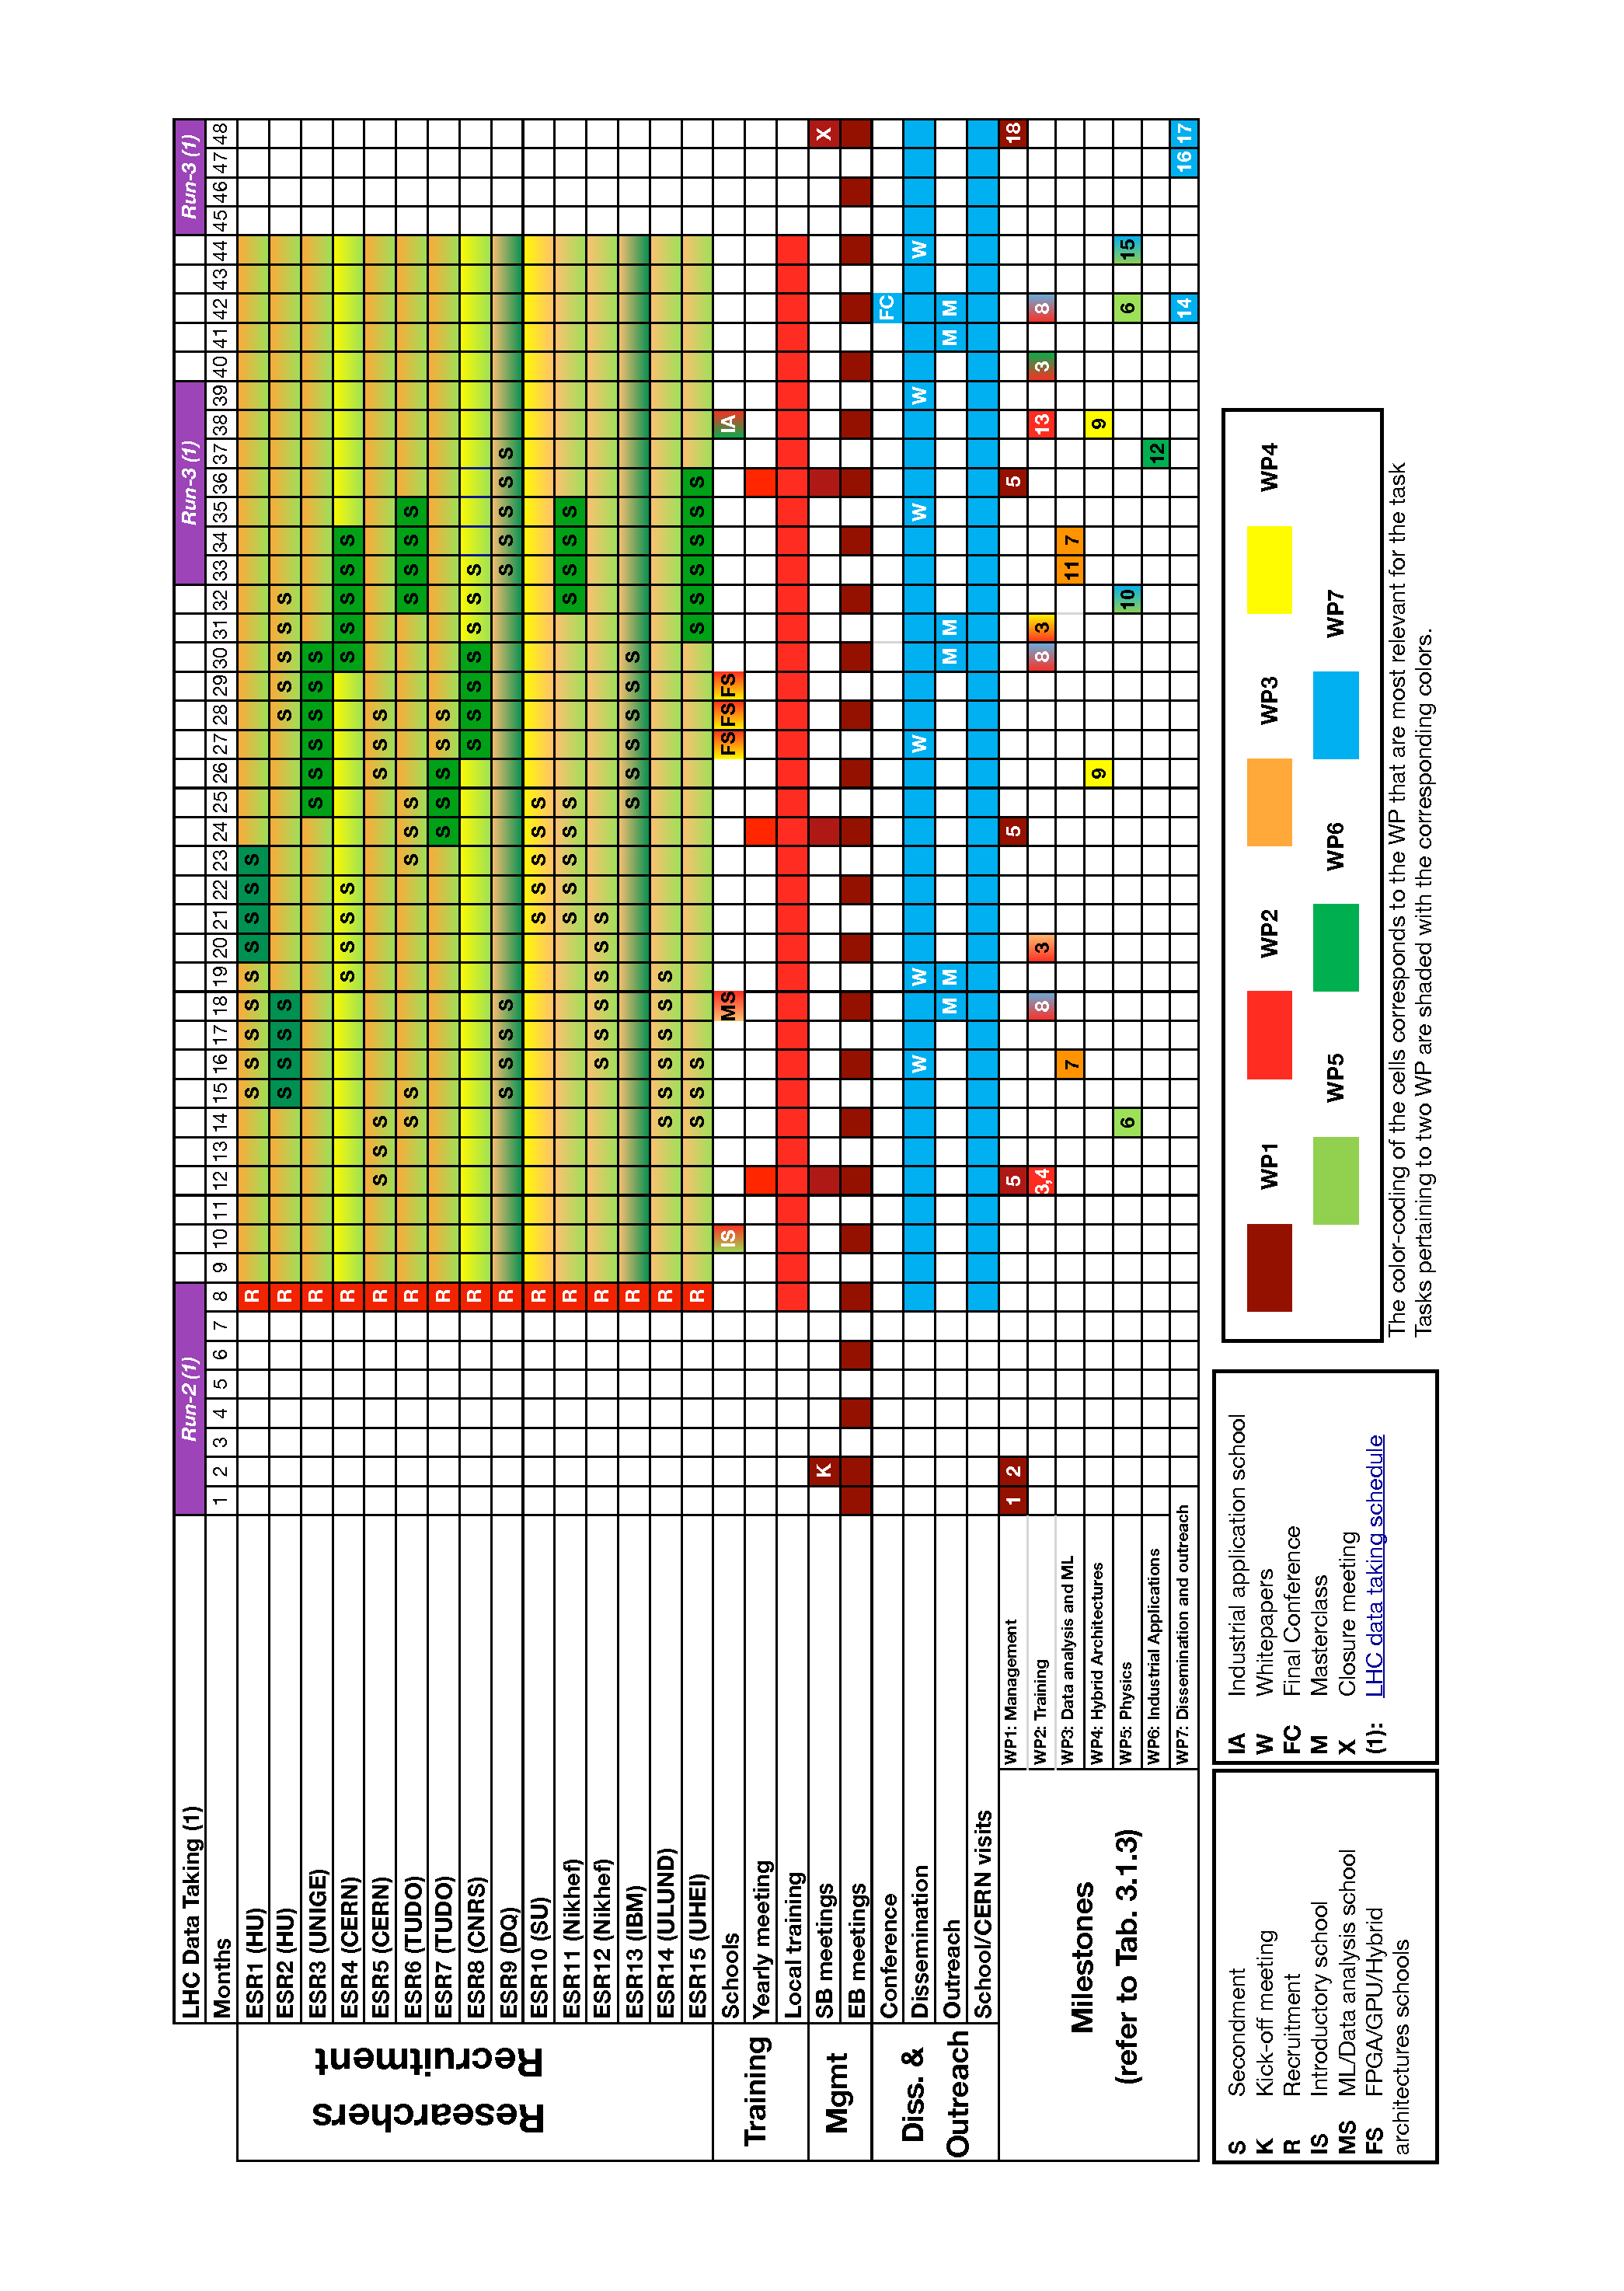
\includegraphics[width=0.9\textwidth]{figs/gantt_v2}
}
	%\caption{\small Structure of the Network. \label{fig:network}} 
%\end{textblock*}    
%\end{figure*}

%%%\addcontentsline{toc}{section}{GANTT CHART}

%%%NB: The schedule of the project should be in terms of number of months elapsed from the start.
%%%%\section{GANTT CHART}
%\vspace{2cm}
\clearpage
%\phantomsection
%\stepcounter{section}
%\addcontentsline{toc}{section}{\protect\numberline{\thesection}GANTT CHART}
\captionsetup[figure]{justification=justified,singlelinecheck=false}
\begin{figure}[p]
\vspace{-5mm}
\begin{flushleft}
\caption*{\textbf{\large 4 GANTT CHART\vspace{-5mm}}
\label{sec:gantt}}
\end{flushleft}
\begin{center}
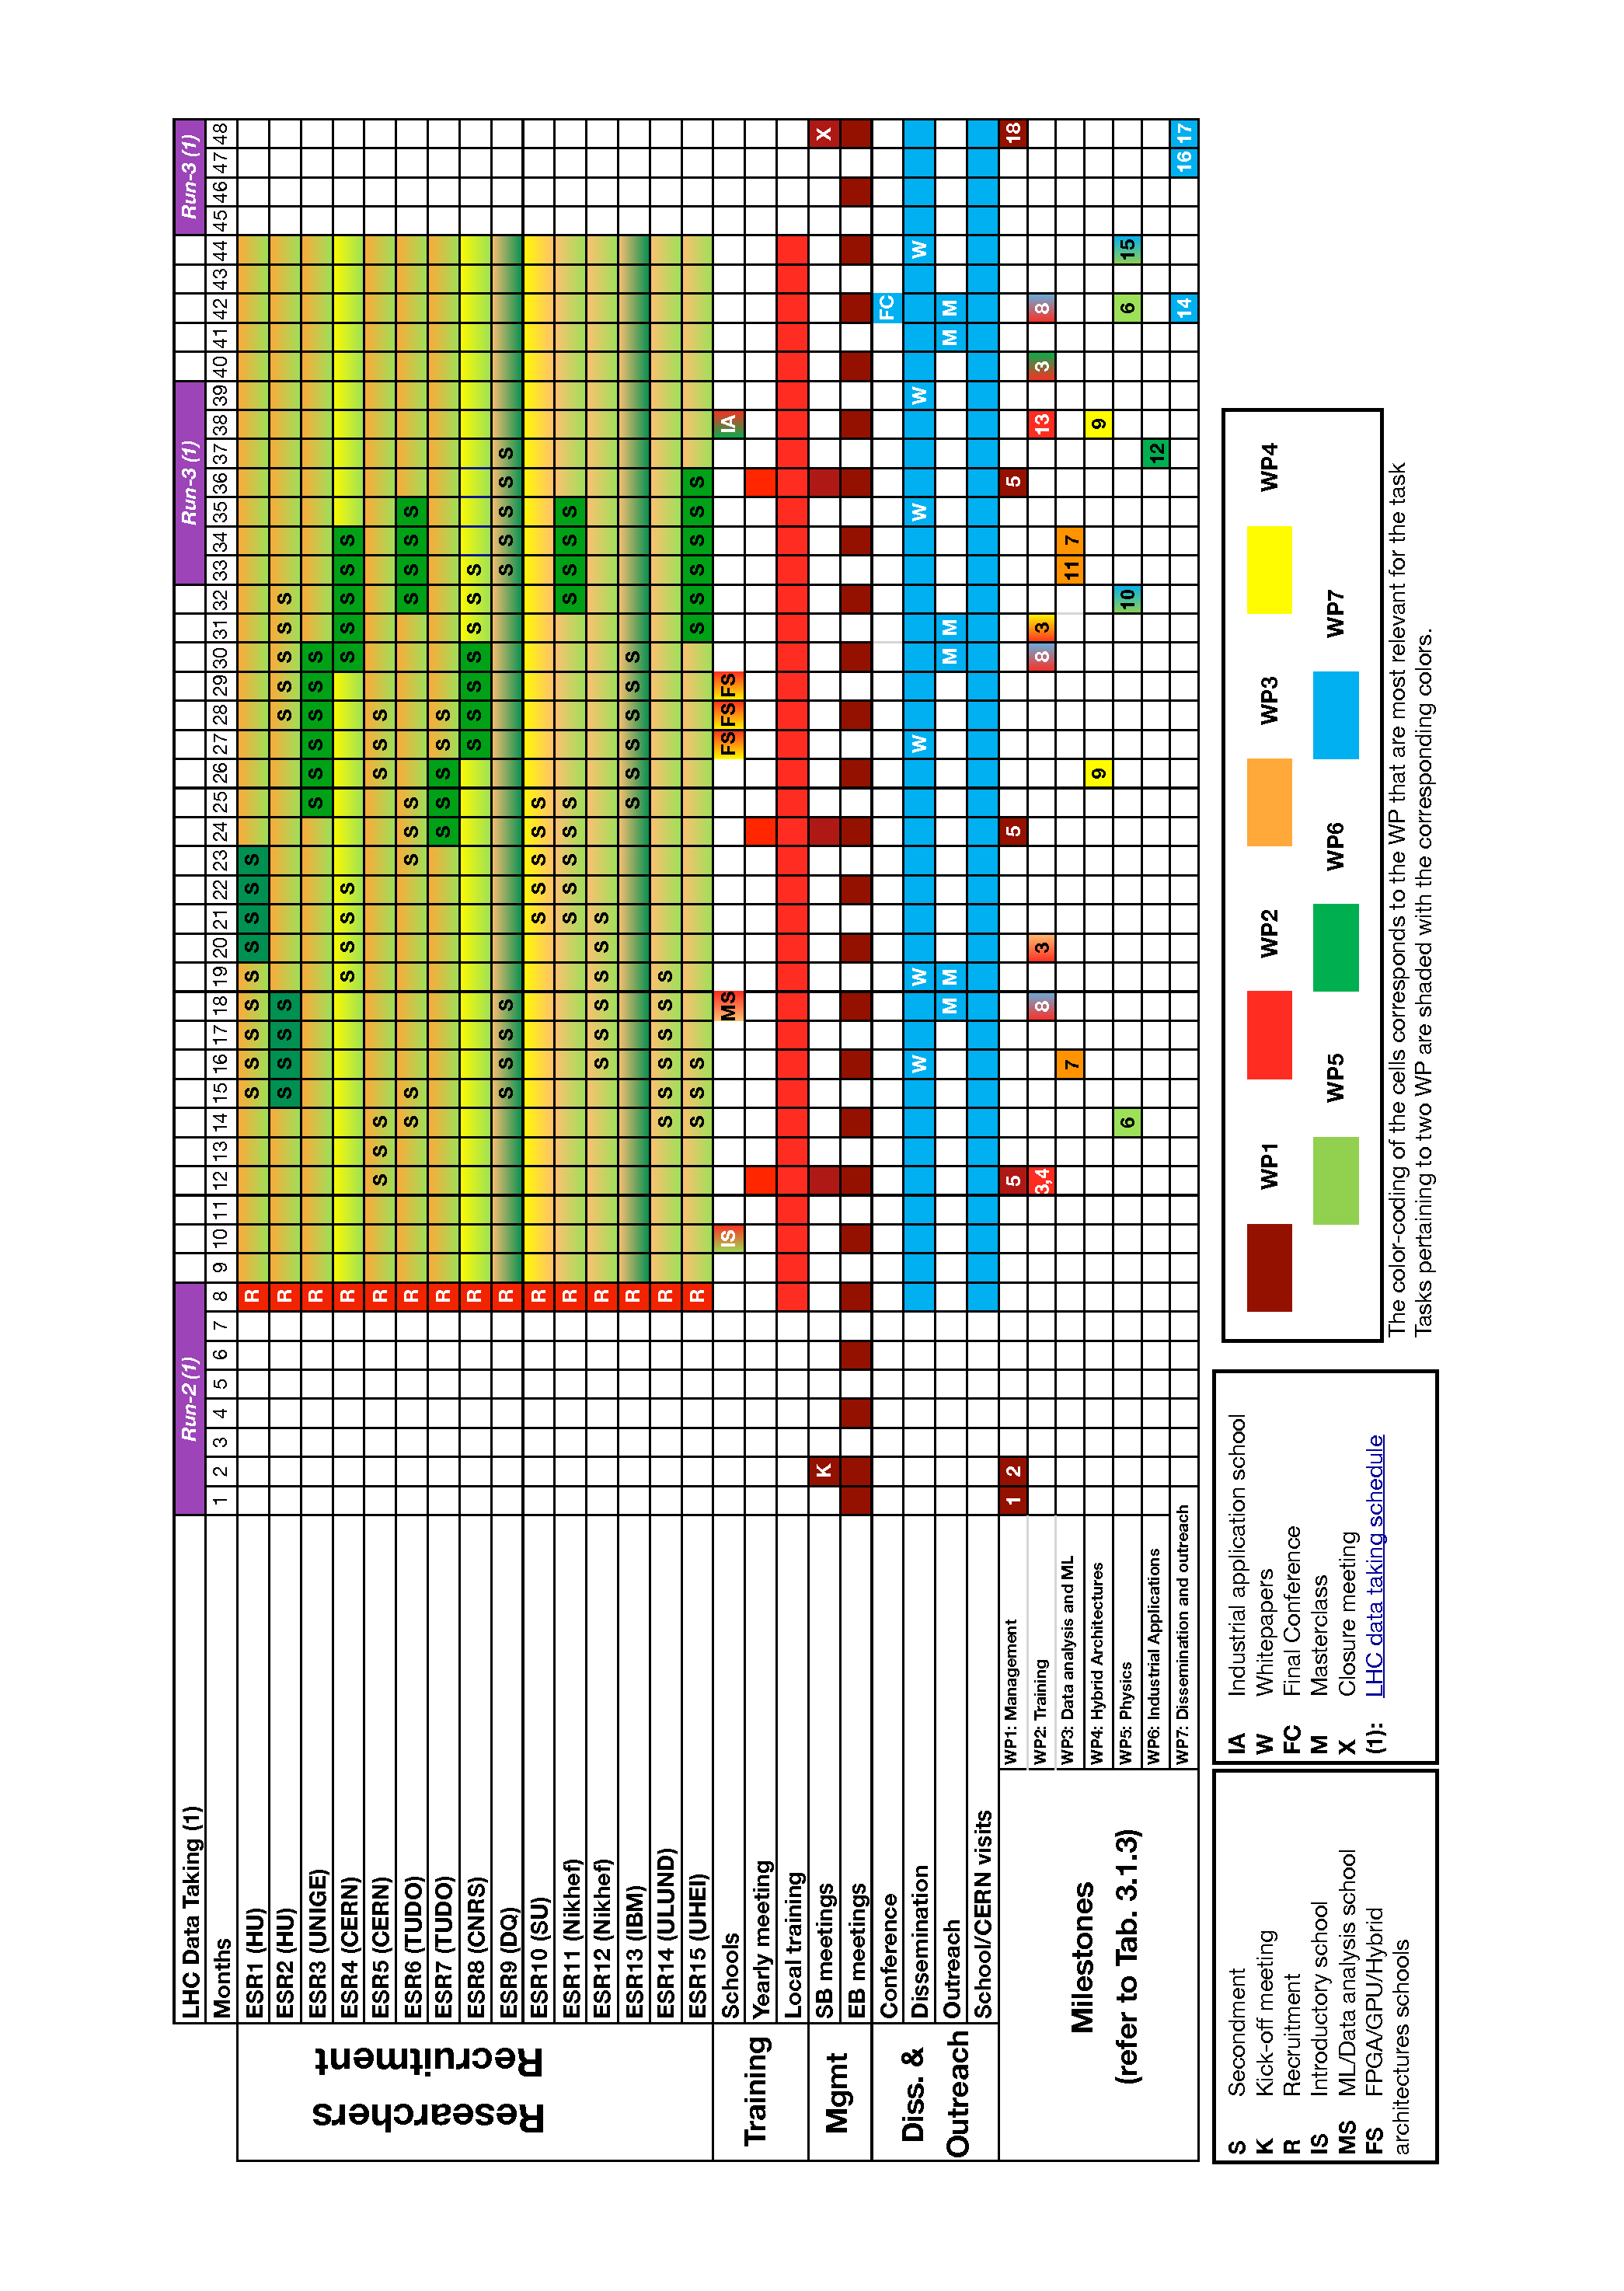
\includegraphics[width=0.835\paperwidth]{figs/gantt_v2.pdf}
\end{center}
\end{figure}
\clearpage\newpage

%%

\clearpage 

\section{CAPACITIES OF THE PARTICIPATING ORGANISATIONS}

\label{sec:capacities}
%%All organisations (whether beneficiaries or partner organisations) must complete the appropriate table below. Complete one table of maximum one page per beneficiary and half a page per partner organisation (minimum font size: 9). 
%
%For beneficiaries:
%
%Beneficiary Legal Name:
%General Description:
%Short description of the activities relevant to the action
%Role and Commitment of key persons (including supervisors):
%Including names, title and the intended extent of involvement in the action - in percentage of full-time employment - of the key scientific staff who will be involved in the research, training and supervision
%Key Research Facilities, Infrastructure and Equipment:
%Outline the key facilities and infrastructure available and demonstrate that each team has sufficient capacity to host and/or offer a suitable environment for supervising the research and training of the recruited Early-Stage Researchers
%Status of Research Premises:
%Please explain the status of the beneficiary's research facilities ? i.e. are they owned by the beneficiary or rented by it? Are its research premises wholly independent from other beneficiaries and/or partner organisations in the consortium?
%Previous Involvement in Research and Training Programmes: 
%Detail any relevant EU, national or international research and training actions/projects in which the beneficiary has previously participated
%Current Involvement in Research and Training Programmes:
%Detail any relevant EU, national or international research and training actions/projects in which the beneficiary is currently participating
%Relevant Publications and/or Research / Innovation Product (Max 5)
%
%For partner organisations:
%
%Partner Organisation Legal Name: 
%General description
%Key Persons and Expertise
%Key Research Facilities, Infrastructure and Equipment
%Previous and Current Involvement in Research and Training Programmes 
%Relevant Publications and/or Research / Innovation Product (Max. 3)


\begin{center}
%\resizebox{\textwidth}{!}{%
\footnotesize
\begin{tabular}{@{}p{25mm}|p{190mm}@{}}
\toprule
\multicolumn{2}{c}{\large\textbf{Beneficiary: \lundlong}}\tabularnewline\hline
\pbox{8cm}{\Tstrut General\\Description\Bstrut} & %
\pbox{19cm}{\Tstrut \lundlong was founded in 1666,
% and for a number of years has been ranked among the world’s top 100 universities~\footnote{See \href{http://www.lunduniversity.lu.se/about/about-lund-university/university-world-rankings}{http://www.lunduniversity.lu.se/about/about-lund-university/university-world-rankings}}. 
the University has 42\,000 students and more than 7\,500 staff based in Lund, Helsingborg and Malmoe. 
The Faculty of Science conducts research and education within Biology, Astronomy, Physics, Geosciences, Chemistry, Mathematics and
Environmental Sciences. 
%The Faculty is organized into ten departments, gathered in the
%northern campus area. 
The Faculty has approximately 1\,900 students, 330 PhD students and 700 employees. 
The Department of Physics is with a staff of about 350 scientists and educators one of the largest departments within \lundlong. 
There are seven research divisions and a number of research centers within the department. 
The research activities at the department cover a broad spectrum of modern physics.
% For more information, see \url{www.fysik.lu.se/english}.  
\Bstrut}\tabularnewline\hline

\pbox{8cm}{\Tstrut Role and\\Commitment\\of Key persons} & %
{\vspace{-8mm}
\begin{enumerate}%[topsep=0pt,itemsep=-2pt,leftmargin=*]
\item Dr.~Caterina Doglioni, physics, senior associate lecturer, 
%convener of ATLAS Exotics jet+X physics group (2012-2014), 
convener of HEP Software Foundation Trigger and Reconstruction working group (2018-present), LHC Physics Center Dark Matter working group organizer (2015-2018), ATLAS Astroparticle forum (2014-2016), 
receiver of ERC Starting Grant 2015 (DARKJETS, Grant Agreement no. 679305) and Swedish Research Council Starting (2015) and Project (2018) grants. 
Expertise in jet reconstruction, dark matter, triggering, real-time analysis in ATLAS.
\textbf{Role:} Project Coordinator, supervisor of \ESRj, tutoring of seconded students. Commitment: 30\%.
\item Dr.~Peter Christiansen, physics, professor of experimental particle physics, expert in real-time detector reconstruction and analysis for the ALICE experiment. Receiver of Wallenberg Project grant CLASH and of Swedish Research Council Project grant (2017). 
\textbf{Role:} supervisor of \ESRk, lectures and organization of training, commitment: 20\%. 
\item Dr.~Oxana Smirnova, physics, associate professor of experimental particle physics, computing grid and distributed data analysis expert, Grid Architect in 2002-2003 and Sweden's representative in the International Computing Board. Receiver of Swedish Research Council Project grant (2017). 
\textbf{Role:} tutoring of seconded students, commitment: 20\%.
%\vspace{-\belowdisplayskip}
\end{enumerate}} \tabularnewline\hline

\pbox{8cm}{\Tstrut Key Research\\Facilities,\\Infrastructure\\and Equipment} & %
\pbox{19cm}{\Tstrut Lund University is active with a strong, long-term contribution to the ATLAS Experiment and the ALICE Experiment.
This ITN fits well the research interests and existing efforts in the group: an ongoing ERC StG, held by Doglioni, includes real-time data analyses
in searches for new physics in jet final states.   
The opportunities for collaboration within the group are strong as the ESRs in this project extend the research program, and there is sufficient room for a clearly defined, original line of research for the students in this project.   
The expertise that can be found in the theoretical physics department of Lund is also invaluable for all physics searches and measurements
in this ITN: the \textsc{Pythia} event generator developed in Lund is the most used for the simulation of both signal and background 
events for jet searches in the ATLAS Collaboration. 
In \lundlong, the ESRs will also benefit from the use of a computing cluster connected to the NorduGrid network, which can be used for fast and efficient data analysis. 
The combination of a strong understanding of the theoretical issues for the comparison of collider Dark Matter searches and a hands-on experience with LHC data will be conducive to developments and collaboration between the beneficiaries of this project, other Swedish Universities contributing to Dark Matter searches within ATLAS and the Swedish NORDITA Dark Matter program that can be undertaken during and beyond the time frame of this project. 
Furthermore, there are two major research facilities in Lund: MAX IV, a world-leading synchrotron radiation laboratory which has opened in 2016, and the European Spallation Source (ESS), a European facility that will host the most powerful neutron source. 
We plan to exploit existing collaborations with researchers at ESS and MAX IV though on the topics within this ITN, allowing cross-pollination of ideas from the visiting researchers and industrial partners that will be beneficial for the training of students resident or seconded in Lund within and beyond the network.
} \tabularnewline\hline
%
\multicolumn{2}{l}{\hspace{-1ex}Independent \Tstrut  research premises\Bstrut: yes}\tabularnewline\hline
\pbox{8cm}{\Tstrut Past \& current\\involvement\\in Research and\\Training\\Programmes} & 
\pbox{19cm}{\Tstrut \lundlong has been and is currently involved in several EU funded projects, in a number of disciplines, hosting several ERC (starting and advanced) grants. 
One of them is the Doglioni's DARKJETS ERC, concerning discovery strategies for Dark Matter and other new phenomena at the LHC, which has a connection to this project. 
Lund particle physics is directly involved in the INSIGHTS ITN (GA No.765710), concerning statistics for physics and society, with which \acronym plans to collaborate in co-organizing a training event. 
Even though Doglioni was the original \lundentity responsible for INSIGHTS, the role of local node coordinator has been assigned to Else Lytken, allowing Doglioni to have time to be PC of \acronym if funded. 
We also plan to collaborate with the~\href{http://www.montecarlonet.org/}{MCNet ETN}, that has a long tradition in Lund.} \tabularnewline\hline\Tstrut
\pbox{8cm}{\Tstrut Relevant\\Publications} &%
{\vspace{-3mm}
\begin{description}%[topsep=0pt,itemsep=-2pt,leftmargin=*]

\item [O. Buchmueller, C. Doglioni and L.T. Wang] Search for dark matter at colliders. Nature Physics 13, 217223 (2017). 
%
\item [ATLAS Collaboration, C. Doglioni and M. Dunford as editor and A. Boveia as analysis contact] Search for low-mass dijet resonances using trigger-level jets with the ATLAS detector in pp collisions at $\sqrt{s}$=13 TeV, Phys. Rev. Lett. 121, 081801 (2018). 
%%Performance of the ATLAS Trigger System in 2015. Eur.Phys.J. C77 (2017) no.5, 317
%
\item [ALICE Collaboration] The ALICE TPC, a large 3-dimensional tracking device with fast readout for ultra-high multiplicity events. Nucl. Instrum. Meth. A 622, 316 (2010) 1
%
\item [ALICE Collaboration] Centrality dependence of the nuclear modification factor of charged pions, kaons, and protons in Pb-Pb collisions at $\sqrt{s_NN}$=2.76 TeV. Phys. Rev. C 93, 034913 (2016)
%
%%Search for new phenomena in dijet mass and angular distributions from $pp$ collisions at  $\sqrt{s}=13$~TeV with the ATLAS detector
%%[ATLAS Collaboration]. Physics Letters B 754 (2016) 302-322
%
%%\item (2015) Search for new phenomena in the dijet mass distribution using $pp$ collision data at $\sqrt{s}=8$~TeV with the ATLAS detector
%%[ATLAS Collaboration]. Phys.Rev. D91 (2015) 052007

\item [O. Smirnova] Current Grid operation and future role of the Grid, in Proceedings of CHEP 2012, J. Phys.: Conf. Ser. 396 042055 (2013)

%Published in \href{http://10.1140/epjc/s10052-014-3190-y}{}. 

\end{description}}\tabularnewline\bottomrule

\end{tabular}
%}%
\end{center}

%\begin{center}
\resizebox{\textwidth}{!}{%
\begin{tabular}{@{}p{25mm}|p{190mm}@{}}
\toprule
\multicolumn{2}{c}{\large\textbf{Beneficiary: \cern}}\tabularnewline\hline
\pbox{8cm}{\Tstrut General\\Description\Bstrut} & %
\pbox{19cm}{\Tstrut 
\cern is an International European Organization and is the worlds largest particle physics centre, providing technologically-advanced facilities for particle physics. 
CERN has 22 member states. 
Close to 13,000 scientists from 650 institutes worldwide are involved in the research and technology programme. 
CERN's mission is focused on 4 topics: research, technology, collaboration and education, including a long and strong training tradition via the Fellows, Associates and Students programmes. 
It has its own Learning and Development service providing almost 14,000 person days of technical management, communication, academic, safety and language training per year. 
The Large Hadron Collider, the largest and most powerful human-made particle collider, is located at CERN, together with its four main experiments: ALICE, ATLAS, CMS and LHCb. 
Researchers from all four collaborations, who spearheaded real-time analysis in their own experiments, are involved in \acronym.  
CERN hosts the largest particle accelerator in the world, the Large Hadron Collider (LHC), which generates data rates of over 100~Exabytes per year.  
CERN's aims include education and it offers a number of educational and training  programmes to students and teachers, as well as playing a leading role in the International Masterclass programme. 
\Bstrut}\tabularnewline\hline
\pbox{8cm}{\Tstrut Role and\\Commitment\\of Key persons} & %
{\vspace{-8mm}
\begin{enumerate}%[topsep=0pt,itemsep=-2pt,leftmargin=*]
\item Dr.~Monica Pepe-Altarelli is a senior physicist at CERN and a member of the LHCb collaboration in which she held several positions of responsibility.
She is Vice-President Elected at Large of the Executive Council of the International Union of Pure and Applied Science  (\href{http://iupap.org/executive-council-and-commission-chairs/executive-council-officers-2017-2020/}{IUPAP}) as well as Associate Member Delegate to the EPS Council for the period April 2017-2021. She has expertise in data analysis in the NA32, ALEPH and LHCb collaborations.
% Dr.~Monica Pepe-Altarelli, CERN staff. She has been LHCb deputy spokesperson and member of LHCb's Gender, Equality, and Diversity task force. 
%She has also been Vice-President Elected at Large of the Executive Council of the International Union of Pure and Applied Science 
%(\href{http://iupap.org/about-us/executive-council/executive-council-officers-2014-2017/}{IUPAP}).
% Expertise in data analysis in NA32, ALEPH and LHCb.
Role: supervision and mentoring of visiting students, lectures. 
Committment: 10\%.
\item Dr. Rosen Matev, CERN LD staff, expertise in software and trigger design and maintenance, RTA, luminosity measurements. 
Has co-supervised three PhD and a MSc student, currently co-supervising a CERN doctoral student. 
Received LHCb Early Career Scientist award, shared with four other colleagues, on the Run II software trigger. 
Role: co-supervisor of \ESRd.
Commitment: 20\%.
\item  Dr. Benjamin Couturier, CERN staff. After graduating from the Ecole Superieure d'Electricite (Supelec) and the University of Paris-Sud in 1996, Benjamin Couturier has been working as Software Engineer and Software Architect for various companies before joining CERN. He is now part of the team developing the software framework used to process and analyze data from the LHCb experiment at CERN.
Role: co-supervisor of \ESRg and \ESRi, lectures, non-academic training.
Commitment: 20\%.
\item Dr. Andrey Ustyuzhanin is the head of Yandex-CERN joint projects as well as the head of Laboratory of Methods for Big Data Analysis at National Research University Higher School of Economics. 
%His team participates in LHCb and SHiP (Search for Hidden Particles). 
He is an expert in machine learning and gives regular lectures on Machine Learning applied to High Energy Physics. % at the Yandex School of Data Analysis. 
Role: lectures, data challenge responsible, non-academic training.
Commitment: 10\%. 
\item Dr. Brian Petersen is a CERN staff scientist, and a member of the ATLAS collaboration. 
He has been the coordinator of the ATLAS trigger group of the ATLAS upgrade physics group.
He has supervised multiple CERN fellows and was chair of the 2017 CERN-Fermilab Hadron Collider Physics Summer School.
Role: supervisor of \ESRc and seconded students, lectures, commitment: 20\%
\item Dr.~Maurizio Pierini is the coordinator of the Physics Performances and Dataset (PPD) area in CMS, and the initiator of the Data Scouting analyses at the trigger level in CMS. 
He is a CERN staff scientist, and a LPC Distinguished Researcher of the Fermilab Physics Center.  
Role: co-supervisor of \ESRa, lectures.
Commitment: 15\%
\item Dr. Ruben Shahoyan is an expert on software and coordinates the reconstruction and calibration activities within the  O2 software project for ALICE Run3/4 upgrade. 
He coordinates the ALICE upgrade activity on calibration and reconstruction, and has played a critical role in calibrating the space point distortions of the existing Time Projection Chamber.
Role: co-supervisor of \ESRk, lectures.
Commitment: 15\%
\vspace{-3mm}
\end{enumerate}} \tabularnewline\hline
\pbox{8cm}{\Tstrut Key Research\\Facilities,\\Infrastructure\\ and Equipment} & %
\pbox{19cm}{\Tstrut World-class accelerator facilities: PS / SPS / LHC complexes. 
In-house engineering/technology/detector physics groups, prototyping, material science services, mechanical and electronics workshop, etc.
Due to its position as a focal point for research into elementary particle physics and associated technologies, CERN has state-of-the-art technological infrastructure and equipment. 
This spans a very large range of facilities such as accelerators and particle detectors, a forefront informatics backbone including Grid developments, state-of-the-art laboratories for mechanical, electronic, microelectronic and optoelectronic engineering and large cryogenics installations.
%In addition to standard office space with fibre-optic network connectivity and a library with access to over 2000 journals relevant to HEP and DS, CERN provides extensive support and infrastructure for both data analysis and computing.
%This includes a 100 node computing cluster and 2~Tb of disk space for each researcher's own work.
%In addition ESRs will have access to a dedicated cluster of around 10 nodes composed of the latest available GPU processors, and a second dedicated cluster of around 10 nodes composed of the latest available CPU 
ESRs will have access to dedicated clusters with the latest available GPU and CPU processors.
} \tabularnewline\hline
\multicolumn{2}{l}{\hspace{-1ex}Independent \Tstrut research premises\Bstrut: Yes
}\tabularnewline\hline
\pbox{8cm}{\Tstrut Past \& current\\involvement\\in Research and\\Training\\Programmes\Bstrut} & 
\pbox{19cm}{\Tstrut 
CERN has a learning and development programme offering about 15 Academic Training courses per year on subjects ranging from theoretical and experimental particle physics, to advances in technologies, computing and engineering. 
%It offers summer programmes for students and high school teachers, including dedicated physics and computing summer schools, as well as technical and doctoral students programmes. 
CERN also has the ``Openlab'' programme collaborating with industry on the development of IT technologies.
CERN has participated in and coordinated numerous European training projects, some recent examples being the ACEOLE, LA3NET, CATHI, EDUSAFE, PACMAN, and ICE-DIP training networks.\\
EU projects (FP7): Coordinator of 15 ITNs (11 completed / 4 ongoing), beneficiary or partner in 14 ITNs ( 8 / 6), coordinator of 5 COFUND grants (4 / 1), coordinator of 2 RISE and benefiociary in 2 RISE. 
%Completed projects : (FP6) Coordinator of 7 EST, 1 RTN, 8 individual fellowships + partner in 2 RTNs; 
% Coordinator of 4 COFUND grants; Coordinator of 15 individual fellowships; partner in 2 IAPPs. 
%Ongoing projects : (FP7) Coordinator of 1 COFUND grant; (H2020) 
%Coordinator of 1 ongoing COFUND grant, coordinator of another grant for a call of more than 50 applicants; Coordinator of 9 ongoing individual fellowships; Coordinator of 2 RISE + beneficiary in 2 others;
}\tabularnewline\hline
\pbox{8cm}{\Tstrut Relevant\\Publications} &%
{\vspace{-3mm}
\begin{itemize}%[topsep=0pt,itemsep=-2pt,leftmargin=*]
\item R. Aaij et al., The LHCb Trigger and its Performance in 2011, JINST {\bf 8} (2013) P04022.
%\item J. Albrecht et al., Event building and reconstruction at 30 MHz using a CPU farm, JINST 9 (2014) C10029
\item R. Aaij et al., Performance of the LHCb trigger and full real-time reconstruction in Run 2 of the LHC, arXiv:1812.10790
\item G.~Aad {\it et al.} [ATLAS Collaboration], Performance of the ATLAS Trigger System in 2010, Eur.\ Phys.\ J.\ C {\bf 72} (2012) 1849
\item M.~Aaboud {\it et al.} [ATLAS Collaboration], Performance of the ATLAS Trigger System in 2015, Eur.\ Phys.\ J.\ C {\bf 77}, no. 5, 317 (2017)
\vspace{-4mm}
\end{itemize}
}\tabularnewline\hline
\end{tabular}
}%
\end{center}
%\begin{center}
\resizebox{\textwidth}{!}{%
\begin{tabular}{@{}p{25mm}|p{190mm}@{}}
\toprule
\multicolumn{2}{c}{\large\textbf{Beneficiary: \dortmundLong}}\tabularnewline\hline 
\pbox{8cm}{\Tstrut General\\Description\Bstrut} &%
\pbox{19cm}{\Tstrut 
TU Dortmund University is hosting more than 34,000 students. 
It has developed a unique profile with particular research strength in natural and engineering sciences, focusing in interdisciplinary and innovative synergies in research. 
The department of Physics has about 50 lecturers and post-doctoral researchers and about 150 PhD students. 
Research focuses are particle physics, solid state physics, and accelerator physics. 
The attractive study program of the department has led to an enormous increase in undergraduate students with currently more than 1,200.
The group "Experimentelle Physik" covers a large area of research in particle physics, focused on data analysis and detector development. 
The group is a member of the LHCb collaboration since 2003 and is central to the development of the High Level Trigger of the experiment and was leading the efforts towards the upgrade trigger Technical Design Report. 
In addition, the group is significantly contributing to the upgraded tracking detector (SciFi-tracker). 
The group is also strongly involved in the core physics analyses of the LHCb experiment. 
Recently, the group intensified its collaboration with the local computer science department by joining the Collaborative Research Center SFB 876 "Providing Information by Resource-Constrained Data Analysis". 
The Initial Training Network proposal fits extremely well with the group's existing research profile on advanced data analysis techniques.
}  
\tabularnewline\hline
\pbox{8cm}{\Tstrut Role and\\Commitment\\ of Key persons} &%
{\vspace{-8mm}
\begin{enumerate}%[topsep=0pt,itemsep=-2pt,leftmargin=*]
\item Dr. Johannes Albrecht, lecturer at the faculty of physics, receiver of an ERC Starting Grant 2016 GA714536 ``PRECISION'' and a Emmy-Noether Grant (2013 - 2018). 
Expertise in track reconstruction, triggering, real time data analysis, multivariate analyses. 
LHCb trigger deputy project leader (2011-2014), LHCb upgrade trigger project leader (2012-2014), physics analysis group convener (2011-2013), physics coordinator (2018-).
Role: supervisor of \ESRd and \ESRe. 
Commitment: 20\%

\item Prof. Bernhard Spaan, head of experimental physics 5, team leader for the LHCb experiment. 
Collaboration board chair of the LHCb experiment (2013-2017). 
Project leader in the computer science special research area
"Providing Information by Resource-Constrained Data Analysis" (SFB876). 
Former Dean of the faculty of physics, former elected head of the
committee of German particle physicists (KET). 
Expertise in data analysis in multiple experiments, including LHCb, BABAR, CLEO and ARGUS. 
Role: senior advisor of supervision of ESR6 and ESR7, commitment: 10\%

\end{enumerate}
}
\tabularnewline\hline   
\pbox{8cm}{\Tstrut Key Research\\Facilities,\\Infrastructure\\and Equipment\Bstrut} & %
\pbox{19cm}{\Tstrut 
The department of physics is involved in data analysis at the CERN based experiments LHCb and ATLAS, in neutrino experiments (Magic, Ice Cube, Cobra) and also has a strong particle physics theory department. 
Students benefit from the close link to the theory part of the department and from the intense collaboration between the department of physics and the department of computer science, which is also formalised in the
participation of two research groups in the Collaborative Research Center (SFB 876). 
The group has access to excellent computing resources, including a local computing cluster and are eligible to perform distributed analysis on the Grid. 
} \tabularnewline\hline 
\multicolumn{2}{l}{\hspace{-1ex}Independent \Tstrut  research premises\Bstrut: yes}\tabularnewline\hline
\pbox{8cm}{\Tstrut Past \& current\\involvement\\in Research and\\Training\\Programmes\Bstrut} &  
\pbox{19cm}{\Tstrut  
The TU Dortmund currently co-ordinates or participates in 36 EU-projects, amongst them 3 Marie-Curie ITNs. 
The group experimental physics 5 participates in the special research area \textit{Providing Information by Resource-Constrained Data Analysis} (SFB876), which ideally complements the proposed ITN. 
Its bi-yearly graduate schools are also open to the members of the ITN. 
The department has an extensive programme on graduate and post-graduate courses. 
Additionally, the local ESRs will become members of the \textbf{Research Academy Ruhr}, one of the largest and most powerful platforms in Germany to support young researchers and prepare them for careers inside and outside academia at the University alliance of three UA Ruhr Universities: Bochum, Duisburg-Essen and TU Dortmund.   
} \tabularnewline\hline\Tstrut
\pbox{8cm}{\Tstrut Relevant\\Publications} &%
{\vspace{-3mm}
\begin{itemize}%[topsep=0pt,itemsep=-2pt,leftmargin=*]
\item The LHCb and CMS Collaborations, Observation of the rare $B^0_s\to\mu^+\mu^-$ decay from the combined analysis of CMS and LHCb data, submitted to Nature.
\item The LHCb and CMS Collaborations, "Observation of the rare $B^0_s \rightarrow \mu^+ \mu^-$ decay", Nature 522 (2015) 68–72
\item R. Aaij, J. Albrecht, et al., "The LHCb Trigger and its Performance in 2011", JINST {\bf 8} (2013) P04022. 
\item  The LHCb Collaboration, "Search for the lepton flavour violating decay $\tau\to\mu\mu\mu$, JHEP 02 (2015) 121
\item The LHCb Collaboration, ``LHCb Trigger and Online Upgrade Technical Design Report'', CERN-LHCC-2014-016
\item The ARGUS Collaboration, "Observation of $B^0-\bar{B^0}$ mixing", Phys.Lett. B192 (1987) 245
\end{itemize}
}\tabularnewline\hline

\end{tabular}
}%
\end{center}
%\begin{center}
\footnotesize
\begin{tabular}{|p{0.1\textwidth}|p{0.85\textwidth}|}
%\resizebox{\textwidth}{!}{%
%\begin{tabular}{@{}p{25mm}|p{190mm}@{}}
\toprule
\multicolumn{2}{c}{\large\textbf{Beneficiary: \nikhef}}\tabularnewline\hline
\pbox{8cm}{\Tstrut General\\Description\Bstrut} & %
\pbox{0.85\textwidth}{\Tstrut \nikhef is the Dutch National Institute for Subatomic Physics, coordinating and 
leading the Dutch experimental activities in the fields of accelerator-based particle physics and 
astroparticle physics, with the mission of studying the interactions and structure of all elementary 
particles and fields at the smallest distance scale and the highest attainable energy. \nikhef is a 
partnership between the Foundation for Fundamental Research on Matter (FOM, part of NWO, the 
Netherlands Organisation for Scientific Research) and four universities: Radboud University 
Nijmegen, University of Amsterdam, Utrecht University and VU University Amsterdam. The research at 
NIKHEF relies on the development of innovative technologies. The knowledge and technology transfer 
to third parties, \ie, industry, civil society and general public, is an integral part of 
\nikhef mission. 
The \nikhef collaboration consists of about 200 physicists (60 tenured staff, 40 postdocs, 100 \phd 
students), 75 technical and engineering staff and 25 support staff and has at present seven 
experimental research lines (ATLAS, ALICE, LHCb, Gravitational Waves, Dark Matter, Neutrino 
Telescopes and Cosmic Rays), and in addition research lines on Theoretical Physics, Detector R\&D 
and Physics Data Processing, supporting the experimental effort. Several members of the tenured staff
also are professor at the partner universities, and through these channels \phd students can be
awarded their doctoral degree at the partner universities.
The FOM-institute \nikhef is located 
in the Amsterdam Science Park. \Bstrut}\tabularnewline\hline
\pbox{8cm}{\Tstrut Role and\\Commitment\\of Key persons} & %
{\vspace{-5mm}
\begin{enumerate}%[topsep=0pt,itemsep=-2pt,leftmargin=*]
\item Prof.~Olga Igonkina, professor of experimental particle
physics in Radboud University of Nijmegen, senior researcher at Nikhef,
ATLAS trigger menu coordinator in Run 1, convener of ATLAS Exotics
lepton+X physics group (2013-2014), receiver of several dutch grants
(VIDI, VICI,  projectruimte). Expertise in $\tau$ reconstruction,
B-physics, lepton flavor violation (LFV), data analysis, triggering.
Role: supervisor of \ESRh, co-supervisor of \ESRi, tutoring of seconded
students, diversity and inclusion officer, commitment: 20\%.
\item Prof.~Gerhard Raven, professor of experimental particle physics, 
former LHCb Trigger project leader, LHCb time-dependent CP-violation physics group convener, 
receiver of several dutch grants. Expertise in data analysis, detector alignment, and triggering.  
Role: supervisor of \ESRi, co-supervisor of \ESRh, tutoring of seconded students, commitment: 20\%;
%\item Dr.~Matt Kenzie, physics, researcher, expertise in data analysis, statistical methods, triggering.  
%Role: co-supervisor of ESR8 and ESR6, tutoring of seconded students, commitment: 20\%;
%\item Dr.~Noam Tal Hod, physics, researcher, ATLAS exotics lepton+X convener (2014-2015), ATLAS exotics trigger liaison. Expertise in data analysis,
%reconstruction and statistics tools.
%Role: tutoring of ESR7 and seconded students, commitment: 20\%.
\vspace{-\belowdisplayskip}
\end{enumerate}} \tabularnewline\hline
\pbox{8cm}{\Tstrut Key Research\\Facilities,\\Infrastructure\\and Equipment} & %
\pbox{0.85\textwidth}{\Tstrut \nikhef has three technical divisions together with 75 staff members: Mechanic Technology (MT), Electronics Technology (ET) 
and Computing Technology CT. \nikhef is equipped with state-of-the-art tools and equipment for engineering design optimisation (3D CAD, material studies, etc.), 
analogue, digital and mixed-signal electronics and micro-electronics design, production and testing (Mentor Graphics, signal generators and analysers, etc.) 
and a powerful computing infrastructure for data processing, consisting of European EGEE Grid clusters and Giga data storage. \nikhef is the Netherlands LHC Tier 1 
and hosts the AMS-IX Internet exchange. \nikhef has  a long tradition in statistical data analysis, and is home to the RooFit Toolkit for data modeling. 
\nikhef also hosts the Particle and Astro-particle track of the joint Physics Master of the two universities of Amsterdam.} \tabularnewline\hline
\multicolumn{2}{l}{\hspace{-1ex}Independent \Tstrut  research premises\Bstrut: yes}\tabularnewline\hline
\pbox{8cm}{\Tstrut Past \& current\\involvement\\in Research and\\Training\\Programmes} & 
\pbox{0.85\textwidth}{\Tstrut \nikhef has been and is currently involved in several EU funded projects, in particular in theory, detector R\&D and e-infrastructure (computing and data processing). \nikhef also hosts several ERC (advanced) grants. NIKHEF is involved in the following Initial Training Networks: MC-PAD (completed), LHCPhenoNet, TALENT, INFIERI and HiggsTools.%
} \tabularnewline\hline\Tstrut
\pbox{8cm}{\Tstrut Relevant\\Publications} &%
{\vspace{-3mm}
\begin{itemize}%[topsep=0pt,itemsep=-2pt,leftmargin=*]
%Removed one paper because we can only quote 5
\item   O.Igonkina for ATLAS collaboration, ``ATLAS trigger menu and performance in Run 1 and
 prospects for Run 2 ``, presented at IEEE 2013, doi:10.1109/NSSMIC.2013.6829554
\item  ATLAS collaboration, O.Igonkina et al., ``Technical Design Report for the Phase-I Upgrade of the ATLAS TDAQ System'', CERN-LHCC-2013-018
\item ATLAS collaboration, O.Igonkina et al., ``Search for new
  phenomena in events with three or more charged leptons in pp
  collisions at $\sqrt{s}=8$ TeV with the ATLAS detector'',
   	JHEP08 (2015) 138
%\item O.Igonkina et al., ``Performance of the ATLAS Trigger System in 2010'', Eur.Phys.J. C72 (2012) 1849
\item J.Albrecht, C.Fitzpatrick, V.Gligorov and G.Raven,  ``The upgrade of the LHCb trigger system'', JINST 9 (2014) C10026
%\item J.Albrecht, V.Gligorov, G.Raven and S.Tolk, ``Performance of the LHCb High Level Trigger in 2012'', J.Phys.Conf.Ser. 513 (2014) 012001.
\item The LHCb collaboration, G.Raven et al., ``Precision measurement of CP violation in $\Bs\to J\psi\Kp\Km$ decays'', Phys. Rev. Lett. 114(2015)041801
% \item    O.Igonkina et al., ``The ATLAS tau trigger'', ATL-DAQ-PROC-2008-008

\end{itemize}}\tabularnewline\bottomrule
\end{tabular}
%}%
\end{center}

%\checkme{PS: Some references seem to be a left-over}

%\begin{center}
\resizebox{\textwidth}{!}{%
\begin{tabular}{@{}p{25mm}|p{190mm}@{}}
\toprule
\multicolumn{2}{c}{\large\textbf{Beneficiary: \unigelong}}\tabularnewline\hline
\pbox{8cm}{\Tstrut General\\Description\Bstrut} & %
\pbox{19cm}{\Tstrut  \unigelong (\unigeshort) is Switzerland's second largest university with more than 17\,000 students of 150 different nationalities and more than 3950 researchers of 113 nationalities, who study and work in 9 different faculties. The university provides an international environment for education and research. It has long history of strong ties with international research organisations, such as \cern. As a result of its history and its strategic choices, the \unigeshort made possible a diversity of research areas to emerge in which the institution excels. High energy physics, profiting strongly from the geographical vicinity to CERN, is one such area of excellence.   
\Bstrut}\tabularnewline\hline
\pbox{8cm}{\Tstrut Role and\\Commitment\\of Key persons} & %
{\vspace{-8mm}
\begin{enumerate}%[topsep=0pt,itemsep=-2pt,leftmargin=*]
\item Prof.~Anna Sfyrla, physics, assistant professor, experimental particle physics and a member of the ATLAS collaboration. She had various responsibility positions at ATLAS in areas spanning the trigger, searches for new physics  and the HL-LHC upgrade. She is currently the thesis director of 1 PhD student, a second one starting in February 2018. She has supervised many PhD, master and summer students in trigger and analysis projects. She has organised, hosted and convened numerous workshops related to her areas of research. More details: \url{http://dpnc.unige.ch/~sfyrla/}. Role: supervisor of ESR2, responsible for WP2. Commitment: 20\%. 
%Coordinator of the ATLAS trigger group between 2014 and 2016 (elected position, about 200 active researchers and students). 
%Coordinator of the Trigger HL-LHC Upgrade Physics\&Performance group (2017). 
%SUSY subgroup convenor between 2013 and 2014.  Expertise in trigger systems and techniques; data analysis; searches for new physics; hadronic object reconstruction. 
%Role: supervisor of ESRXX, co-supervisor of ESRXX, responsible for training within \WP{2}. Commitment: 30\%
% %(in case you need a website: http://dpnc.unige.ch/~sfyrla/)
 \item Dr.~Steven Schramm, physics, senior postdoc, member of the ATLAS Collaboration. He has previously or currently holds positions in areas relating to the trigger, machine learning, and the reconstruction of physics objects used for dark matter searches: ATLAS jet trigger coordinator (2015-2017), convener of ATLAS jet substructure group (2017-present), founder and coordinator of LHC Inter-experimental Machine Learning group (2015-present). Scientific secretary to the ATLAS trigger and data acquisition steering group (2017-present). Recipient of Canadian Banting fellowship. Expertise in jet reconstruction, searches for new physics, machine learning, data analysis, triggering. He has previously and continues to co-supervise many PhD, MSc, and summer students in the areas of triggers, jet performance, and analysis.   
 Role: co-supervisor of ESR2, tutoring of students seconded at CERN. Commitment: 20\%.
% \vspace{-\belowdisplayskip}
\end{enumerate}}
\tabularnewline\hline
\pbox{8cm}{\Tstrut Key Research\\Facilities,\\Infrastructure\\ and Equipment} & %
\pbox{19cm}{\Tstrut  
The Department of Nuclear and Particle Physics of the \unigelong studies the fundamental structures and laws of nature following three complementary directions: collider physics at \cern s LHC; neutrino physics in collider experiments; astroparticle physics experiments on the group and in space. The ATLAS group of the department has made significant contributions to the construction and operation of the experiment. It is presently contributing to event reconstruction and searches for new physics, as well as the HL-LHC upgrade.
\unigeshort has computing clusters available for the ATLAS affiliated students and researchers, comprised of more than 3000 computing cores. The ATLAS group owns several hundreds of TB of disk storage space, as well as high-performance GPUs obtained recently to further the research and development of machine learning tools and real-time applications. 
Many internal training programmes and facilities are available to the ESR affiliated to \unigeshort. The student will have access to the universities Doctoral School, where experimental and theoretical aspects of High Energy Physics at PhD level are taught. The student will also have access to career forums organised by the University of Geneva. 
} \tabularnewline\hline
\multicolumn{2}{l}{\hspace{-1ex}Independent \Tstrut research premises\Bstrut: yes}\tabularnewline\hline
\pbox{8cm}{\Tstrut Past \& current\\involvement\\in Research and\\Training\\Programmes\Bstrut} & 
\pbox{19cm}{\Tstrut 
\unige researchers are granted numerous prizes and distinctions each year. Almost 50 researchers from \unige were granted a prestigious European Research Council Grant (FP7 and H2020).
Open to the world, the \unige leads research projects in collaboration with almost 100 countries. At a European level, the UNIGE actively participates in many EU research programmes, particularly to the Framework Programmes for Research with more than 250 participations in FP7 including 20 coordinations and 36 prestigious European Research Council Grants and over 50 participations in Horizon 2020 projects. \unige is also involved in 50 COST networks and research projects and many other European and international research and innovation programmes (IMI, ESA, INTERREG, NIH, etc.). 
}\tabularnewline\hline
\pbox{8cm}{\Tstrut Relevant\\Publications} &%
{\vspace{-3mm}
\begin{itemize}%[topsep=0pt,itemsep=-2pt,leftmargin=*]
\item   ATLAS Collaboration: ``Search for new phenomena with large jet multiplicities and missing transverse momentum using large-radius jets and flavour-tagging at ATLAS in 13 TeV proton-proton collisions''  JHEP 1712(2017)034
\item  ATLAS Collaboration: ``Jet reconstruction and performance using particle flow with the ATLAS detector''  EPJC 77(2017)466.
\item  ATLAS Collaboration: `Performance of the ATLAS Trigger System in 2015`''  EPJC77(2017)317
\item  ATLAS Collaboration: ``Search for new phenomena in final states with large jet multiplicities and missing transverse momentum at $\sqrt{s}$=8 TeV proton-proton collisions using the ATLAS experiment'' JHEP 10(2013)130
\end{itemize}
}\tabularnewline\hline
\end{tabular}
}%
\end{center}
%\checkme{PS : Maybe one more reference?}
%\begin{center}
\resizebox{\textwidth}{!}{%
\begin{tabular}{@{}p{25mm}|p{190mm}@{}}
\toprule
\multicolumn{2}{c}{\large\textbf{Beneficiary: \heidelberglong}}\tabularnewline\hline
\pbox{8cm}{\Tstrut General\\Description\Bstrut} & %
\pbox{19cm}{\Tstrut  
\heidelberglong  was established in 1386 and is  oldest university in Germany.  It is also one of the strongest research universities in Europe. 
\heidelberglong has twelve faculties with a total of more than 30,000 students and a research and teaching staff of more than 5,000 scientists - among them 450 professors. The Department of Physics and Astronomy follows the idea of teaching rooted in research and sees its research programme at the borders of knowledge as a pre-requisite for teaching and training its students at high quality. The Kirchhoff Institute for Physics performs the research in the areas of classic complex systems, quantum systems as well as in fundamental particles and interactions domain.  It continues the tradition of diverse scientific research and education.  
\Bstrut}\tabularnewline\hline

\pbox{8cm}{\Tstrut Role and\\Commitment\\of Key persons} & %
{\vspace{-8mm}
\begin{enumerate}%[topsep=0pt,itemsep=-2pt,leftmargin=*]
\item Dr.~Pavel Starovoitov is a postdoctoral researcher  at the \hd, and a member of the ATLAS Collaboration since 2000. He is leading the Tile Calorimeter Upgrade Simulation group of the ATLAS experiment.  He was the convener of the PDF Fit Forum and of the Jets and Photon Physics working group  in  ATLAS Collaboration. He has been the second supervisor of 1 PhD student at the University of Hamburg,  1 PhD student at the Heidelberg University, and currently supervises 1 PhD student at the Belarus State University and co-supervises 4 PhD students at the Heidelberg University. He has co-supervised several Master and Bachelor students. Dr.~Starovoitov was the holder of the  Marie-Curie Incoming International Fellowship, CERN-INTAS Young Scientist Fellowship.
%
Role: main supervisor of ESR15 and coordinator of the WP6: "Industrial applications". Commitment: 30\%. 
\item Priv.~Doz.~Dr.~Monica Dunford is a young researcher group leader at the University of Heidelberg. She has been a member of the ATLAS collaboration since 2006 and has been active in the hadronic calorimeter, the trigger system, precision measurements of the Standard Model as well as searches for Dark Matter. She was also a member of the SNO collaboration, where she did hardware development and energy reconstruction algorithms for Cherenkov detectors. She has supervised or co-supervised eight PhD students in addition to many masters and bachelors students. She is on the programming boards for several international conferences in LHC physics.
Role: co-supervisor of ESR15. Commitment: 10\%. 
%\vspace{-\belowdisplayskip}
\end{enumerate}
} 
\tabularnewline\hline
\pbox{8cm}{\Tstrut Key Research\\Facilities,\\Infrastructure\\and Equipment} & %
\pbox{19cm}{\Tstrut %}\tabularnewline\hline
%
\hdshort ATLAS group has its own computing farm with about 500 worker nodes and 600TB disk space for a fast local data analysis. 
The farm is connected to the Worldwide HEP grid network as well as to the German national analysis facility (NAF) with several thousands computing cores and Petabytes of disk space. Students will benefit from enrollment in the Heidelberg graduate schools for fundamental Physics that combines doctoral projects from the forefront of international research with a broad and deep 
teaching program in these areas of fundamental physics and emphasizes their interrelations, as well as from strong connections to the Institute of Theoretical Physics, performing 
research in QCD phenomenology, Dark Matter particles and Higgs Physics domains. 
%
\hdshort has fully equipped electronics laboratory with clean room, component placer, high-frequency oscilloscopes, etc. There are ten electronics engineers, two of them work 100\% with the ATLAS group.
} \tabularnewline\hline
%
\multicolumn{2}{l}{\hspace{-1ex}Independent \Tstrut  research premises\Bstrut: yes}\tabularnewline\hline
\pbox{8cm}{\Tstrut Past \& current\\involvement\\in Research and\\Training\\Programmes} & 
\pbox{19cm}{\Tstrut  
All PhD students from the \hdshort ATLAS group are enrolled in the Heidelberg Graduate School of Fundamental Physics (HGSFP). In addition to providing excellent  education in astronomy and cosmics physics, particle physics, quantum dynamics,	cosmology, mathematical physics, HGSFP  aims to train young scientists to be able to  cross the boundaries between different fields of fundamental physics. 
The \heidelberg participates in  112  projects within FP7 and 49 projects within H2020 programs, where it leads 49 and 26 projects respectively. It includes both collaborative and individual grants.  %For example, The \hdshort group has running EU FP7 training network grant PicoSEC-MCNet 
} \tabularnewline\hline\Tstrut
\pbox{8cm}{\Tstrut Relevant\\Publications} &%
{\vspace{-3mm}
\begin{itemize}%[topsep=0pt,itemsep=-2pt,leftmargin=*]
\item   ATLAS Collaboration: ``Measurement of inclusive jet and dijet cross-sections in proton-proton collisions at $\sqrt{s}=13$ TeV with the ATLAS detector'' arXiv:1711.02692
\item  ATLAS Collaboration: ``Measurement of differential cross sections and $W^+/W^-$  cross-section ratios for $W$ boson production in association with jets at $\sqrt{s}=8$ TeV with the ATLAS detector'' arXiv:1711.03296
\item   ATLAS Collaboration: ``Measurement of three-jet production cross-sections in $pp$ collisions at 7 TeV centre-of-mass energy using the ATLAS detector'' EPJC 75(2015)228
\item   ATLAS Collaboration: ``Measurement of detector-corrected observables sensitive to the anomalous production of events with jets and large missing transverse momentum in $pp$ collisions at $\mathbf{\sqrt{s}=13}$  TeV using the ATLAS detector'' EPJC 77(2017)11
\item   ATLAS Collaboration: ``Jet energy scale measurements and their systematic uncertainties in proton-proton collisions at $\sqrt{s} = 13$ TeV with the ATLAS detector'' Phys.Rev.D 7(2017)072002
\end{itemize}}\tabularnewline\bottomrule
\end{tabular}
}%
\end{center}


%\begin{center}
\resizebox{\textwidth}{!}{%
\begin{tabular}{@{}p{25mm}|p{190mm}@{}}
\toprule
\multicolumn{2}{c}{\large\textbf{Beneficiary: \helsinkilong}}\tabularnewline\hline
\pbox{8cm}{\Tstrut General\\Description\Bstrut} & %
\pbox{19cm}{\Tstrut The \helsinkilong  is nearly 400 years old and is the leading university in Finland. It was placed number 90 in the most recent Times Higher Education World University Rankings. The University has 40,000 students of which 4,700 are doctoral students (1/4 international) distributed on 32 doctoral programs. The university is a top research university and is e.g. a member of the League of European Research Universities. The Department of Physics is one of the largest departments of the university and has 30 professors and about 330 annual person-years..
\Bstrut}\tabularnewline\hline
\pbox{8cm}{\Tstrut Role and\\Commitment\\of Key persons} & %
{\vspace{-8mm}
\begin{enumerate}%[topsep=0pt,itemsep=-2pt,leftmargin=*]
\item  Dr.~Mikko Voutilainen, Assistant Professor of Experimental Elementary Particle Physics, \helsinkilong. He is a world expert on jet energy corrections and jet measurements, and recipient of two prestigious prices in this field (URA Thesis Award for PhD, and Wu-Ki Tung Award for post-doc). He is project leader of the CMS Experiment project at HIP, co-convener of CMS-SMP-Jets group and PI of the UH project ``Precision measurements of QCD'' and the Academy of Finland project ``Top quarks and gluons''.
 Role: main supervisor of ESR1 and co-supervisor of ESR2. Commitment: 15\% 
\item Dr.~Henning Kirschenmann, Postdoctoral Researcher at the Helsinki Institute of Physics. He has a strong background in jet physics (top mass, jet calibration), searches for new physics (SUSY), and jets at the trigger level. He is currently jet energy correction and resolution subgroup co-convener in CMS and focuses on innovative use of DNNs for improving jet performance.
Role: co-supervisor of ESR1 and ESR2. Commitment: 20\%
\item Dr.~Paula Eerola, Professor of Experimental Elementary Particle Physics, \helsinkilong. Director of Helsinki Institute of Physics. She is a leading expert in all aspects of B physics at LHC-CMS, physics beyond the Standard Model at LHC-CMS. Novel data processing techniques. Application of particle physics detectors to radiation detection. Role: Senior advisor, co-supervisor of ESR2. Commitment: 5\% 
%\vspace{-\belowdisplayskip}
\end{enumerate}
} \tabularnewline\hline
\pbox{8cm}{\Tstrut Key Research\\Facilities,\\Infrastructure\\ and Equipment} & %
\pbox{19cm}{ \helsinkientity is a Tier-2 site in the LHC Computing Grid and extensive local computing resources are available for physics analyses. The \helsinkientity Detector laboratory is playing a critical role in upgrades to the CMS tracker and there is a possibility to cooperate with the local theory community as well  
}
\tabularnewline\hline
\multicolumn{2}{l}{\hspace{-1ex}Independent \Tstrut research premises\Bstrut: yes}\tabularnewline\hline
\pbox{8cm}{\Tstrut Past \& current\\involvement\\in Research and\\Training\\Programmes\Bstrut} & 
\pbox{19cm}{\Tstrut The department of physics has participated in 3 FP7 MSC-ITN (CLOUD-ITN, CLOUD-TRAIN, HEXACOMM) projects and coordinated 2 FP7 IRSES (LAIC, GHG-LAKE) and 1 FP7 IAPP (MeChanICs) projects.
UH is currently participating in 11 H2020 MSC ITN and 8 RISE projects and hosting 19 MSC Individual Fellowships.
The department of physics hosts 4 MSCA-IF (nanoCAVa, OXFLUX, FRoST, LAWINE) projects and is participating in 1 MSCA-RISE (NonMinimalHiggs) project and in 1 MSCA-ITN project (CLOUDMOTION).
}
\tabularnewline\hline
\pbox{8cm}{\Tstrut Relevant\\Publications} &%
{\vspace{-3mm}
\begin{itemize}%[topsep=0pt,itemsep=-2pt,leftmargin=*]
\item (2017) Jet energy scale and resolution in the CMS experiment in pp collisions at 8 TeV. [CMS Collaboration]. JINST 12 (2017) no.02, P02014
\item (2011) Determination of jet energy calibration and transverse momentum resolution in CMS. [CMS Collaboration]. JINST 6 (2011) P11002
\item (2017) Search for dijet resonances in proton–proton collisions at $\sqrt{s}=13$ TeV and constraints on dark matter and other models. [CMS Collaboration]. Phys.Lett. B769 (2017) 520-542
\item (2017) Identification of heavy-flavour jets with the CMS detector in pp collisions at 13 TeV. [CMS Collaboration].  arXiv:1712.07158 [physics.ins-det]
\vspace{-4mm}
\end{itemize}
}\tabularnewline\hline
\end{tabular}
}%
\end{center}
%\checkme{PS: Publications are missing}

%\begin{center}
\footnotesize
\begin{tabular}{|p{0.1\textwidth}|p{0.85\textwidth}|}
%\resizebox{\textwidth}{!}{%
%\begin{tabular}{@{}p{25mm}|p{190mm}@{}}
\toprule
\multicolumn{2}{c}{\large\textbf{Beneficiary: CNRS}}\tabularnewline\hline 
\pbox{8cm}{\Tstrut General\\Description\Bstrut} &%
\pbox{0.85\textwidth}{\Tstrut 
LPNHE is a particle, astroparticle, and nuclear physics laboratory within the IN2P3 institute of CNRS, with around 110 researchers and support personnel. The laboratory participates in several world-wide experiments (ATLAS, LHCb, Auger, LSST, etc.), and local teams are formed around each experiment. The laboratory is attached to the Sorbonne Universite, a recently founded mega-university which is home to around 58000 students and 200 laboratories hosting 7700 professor-researchers and over 5000 doctoral students, as well as over 50 ERC grants and 45 industry sponsored research chairs. This ensures that the \acronym students recruited or seconded to the CNRS node will receive the best and most modern training available. Note that although CNRS does not itself give out PhDs, the embedding of the lab in Sorbonne Universite means that PhD students are hosted in LPNHE, paid by CNRS, and receive their degrees from Sorbonne Universite. 
}
\tabularnewline\hline
\pbox{8cm}{\Tstrut Role and\\Commitment\\ of Key persons} &%
{\vspace{-5mm}
\begin{enumerate}%[topsep=0pt,itemsep=-2pt,leftmargin=*]
\item  Dr.~Vladimir V. Gligorov, senior researcher at LPNHE, is the former LHCb High Level Trigger project leader and deputy Physics Coordinator, and now leads LHCb's Real Time Analysis project (consisting of 30 institutes and around 50 FTE). Together with M. Williams, Gligorov was responsible for the first large scale use of Machine Learning in the trigger system of an LHC experiment, with over 1/3 of LHCb's data between 2010 and 2012 taken using the novel boosted decision tree which they had designed to be safe for real-time use. Gligorov launched and subsequently coordinated LHCb's masterclass programme, and is the PI of ERC Consolidator Grant GA724777 "RECEPT". He has co-supervised one PhD, one Masters, and several CERN summer students and is currently supervising two PhD students. Gligorov's PhD student won the LHCb thesis prize in 2016. Expertise in triggering, real-time reconstruction, machine learning, data analysis, outreach. Role: co-supervisor of \ESRj, LHCb contact person, tutoring of seconded students, ML, AI, and data analysis WP coordinator. Commitment: 20\%
\item Francesco Crescioli, research engineer at LPNHE and member of the ATLAS collaboration. He is an expert in ASIC design and design and commissioning of highly parallel FPGA based reconstruction systems. He has co-lead the development of the Associative Memory (AM) chip for the FTK processor in ATLAS and he is currently the AM representative in the FTK Coordination Board in ATLAS. He is the technical coordinator of the French Agence Nationale de la Recherche project "FastTrack" (ANR-13-BS05-0011). He has been the technical coordinator of the SATT IDF Innov valorization project "SPAD" (no. 268).  He has been the coordinator of the WP6 of the EU IAPP project "FTK" (grant agreement no. 324318). He is the technical coordinator of ATLAS Group at LPNHE. He has co-supervised two Master students, at University of Pisa and LPNHE, and he is currently supervising a small team of engineers. Role: co-supervisor of ESR6, lecturer on hybrid architectures, supervision of seconded students, diversity officer. Commitment: 20\%
\item Bogdan Malaescu, senior researcher at LPNHE and member of the ATLAS collaboration, expert in statistics and physics data analysis with jets. He has been nominated convener of the "Standard Model" group in ATLAS and he has been convener of the "Statistics  Forum", "Jets \& photons" subgroup of the "Standard Model" and "Jet energy scale and jet energy resolution" subgroup of the "JetEtmiss" group. He has been co-supervisor of a PhD student and supervisor of 3 Master students. He is currently co-supervising a PhD student. Role: co-supervisor of ESR6. Commitment: 20\%
\vspace{-2mm}
\end{enumerate}
} \tabularnewline\hline   
\pbox{8cm}{\Tstrut Key Research\\Facilities,\\Infrastructure\\and Equipment\Bstrut} & %
\pbox{0.85\textwidth}{\Tstrut
 The LPNHE lab hosts a large computing cluster, with both x86 and non-x86 (GPU/FPGA/hybrid) architectures, which the researchers can use in their work. LPNHE also has an extensive staff of full-time mechanical and electronics engineers who can provide support to researchers in their work. Further computing resources including personal cloud storage are available through the CNRS cloud computing platforms. Appropriate office space, secretarial, administrative, and outreach support, as well as access to all relevant scientific literature is provided.
} 
\tabularnewline\hline
\multicolumn{2}{l}{\hspace{-1ex}Independent \Tstrut  research premises\Bstrut: yes}\tabularnewline\hline
\pbox{8cm}{\Tstrut Past \& current\\involvement\\in Research and\\Training\\Programmes\Bstrut} &  
\pbox{0.85\textwidth}{
\Tstrut CNRS has hosted 460 ERC grants since 2007 and participated or coordinated over 450 H2020 programmes since 2014. Full lists can be found  \href{http://erc.cnrs.fr/en/tous-les-laureats/}{here} and \href{http://www.fabiodisconzi.com/open-h2020/per-country/fr/centre+national+de+la+recherche+scientifique+cnrs/index.html}{here}. The most relevant grants currently hosted in the participating labs are GA654168 "AIDA-2020" and GA724777 "RECEPT", both part of the H2020 programme.
} 
\tabularnewline\hline\Tstrut
\pbox{8cm}{\Tstrut Relevant\\Publications} &%
{
\begin{itemize}%[topsep=0pt,itemsep=-2pt,leftmargin=*]
\item R. Aaij et al., Tesla : an application for real-time data analysis in High Energy Physics, Comput.Phys.Commun. 208 (2016) 35-42.
%\item V. V. Gligorov, Real-time data analysis at the LHC: present and future, J.Mach.Learn.Res. 42 (2015) 1-18
\item V.V. Gligorov and M. Williams, Efficient, reliable and fast high-level triggering using a bonsai boosted decision tree, JINST 8 (2013) P02013
\item C.L. Sotiropoulou et al., The Associative Memory System Infrastructures for the ATLAS Fast Tracker, IEEE Trans.Nucl.Sci. 64 (2017) no.6, 1248-1254
\item B. Malaescu and P. Starovoitov, Evaluation of the Strong Coupling Constant alphas Using the ATLAS Inclusive Jet Cross-Section Data, Eur. Phys. J. C 72 (2012) 2041
\item M. Aaboud et al. (ATLAS Collaboration), Search for new phenomena in dijet events using 37 fb-1 of pp collision data collected at 13 TeV with the ATLAS detector, Phys. Rev. D 96 (2017) no.5,  052004
%Had to remove one because we're up to 5
%\item M.Ali Mirzaei et al., Heterogeneous computing system platform for high-performance pattern recognition applications, proceedings of MOCAST 2017
\end{itemize}
}\tabularnewline\hline
\end{tabular}
%}%
\end{center}

%\checkme{List of Publications}

%\begin{center}
\footnotesize
\begin{tabular}{|p{0.1\textwidth}|p{0.85\textwidth}|}
%\resizebox{\textwidth}{!}{%
%\begin{tabular}{@{}p{25mm}|p{190mm}@{}}
\toprule
\multicolumn{2}{c}{\large\textbf{Beneficiary: \parisUlong}}\tabularnewline\hline
\pbox{8cm}{\Tstrut General\\Description\Bstrut} & %
\pbox{0.85\textwidth}{\Tstrut 
Born from the merger of Universite Pierre et Marie Curie and \parisUlong, whose campuses are in the heart of Paris, \parisUlong covers all major disciplinary fields and offers new 
transversal academic and research programs. \parisUlong becomes a fully multidisciplinary research-intensive university with three faculties: Humanities and Social Sciences, Medicine  and Sciences \& Engineering. With more than 53 400 students (among 10 200 international  students), 4400 doctoral students and 6300 researchers, \parisUlong is one of the leading  French universities. The university is involved in numerous European and International partnership agreements and has France's largest scientific library and infrastructures bringing together the best talent in a wide array of these disciplines. With 8,500 publications per year (approx. 10\% of all publications in France), \parisUlong is a major player in international knowledge and innovation economy, offering transversal academic and research programs. The EU office will manage all the financial, administrative and legal aspects for the participation of \parisUlong in this project. 
\Bstrut}\tabularnewline\hline

\pbox{8cm}{\Tstrut Role and\\Commitment\\of Key persons} & %
{\vspace{-5mm}
\begin{enumerate}%[topsep=0pt,itemsep=-2pt,leftmargin=*]
\item Prof. Lionel Lacassagne, full professor at \parisUlong, leader of the Hardware and Software for Embedded Systems team at LIP6. 
Expertise in designing embedded systems and highly parallel heterogeneous computing architectures. Role: coordinator of hybrid architectures WP, supervisor of \ESRg and co-supervisor of \ESRm, lecturer on hybrid architectures, supervision of seconded students. Commitment: 20\%
\item Prof. Quentin Meunier, associate professor at \parisUlong, expert in architectures and software for efficient parallelisation, including cache protocols, coherence management, fixed-point and floating-point arithmetic. Role: additional supervision of \ESRg and \ESRm and seconded students. Commitment: 20\%

\item Prof. Andrea Pinna, associate professor at \parisUlong, expert in algorithm (Symbolic, NNs, CNN, Fuzzy logic three) implementation for embedded system architecture, digital VLSI system design, CMOS vision system on chip. Role: additional supervision of \ESRg, \ESRm and seconded students.  Commitment: 20\%
\vspace{-2mm}%\belowdisplayskip}
\end{enumerate}} \tabularnewline\hline

\pbox{8cm}{\Tstrut Key Research\\Facilities,\\Infrastructure\\and Equipment} & %
\pbox{0.85\textwidth}{\Tstrut 
The LIP6 lab hosts a large computing cluster, with both x86 and non-x86 (GPU/FPGA/hybrid) architectures, which the researchers can use in their work. The lab also has extensive facilities for designing new computing architectures, with dedicated support from a team of full-time experienced engineers for the work of researchers. Further computing resources including personal cloud storage are available, and access to all relevant scientific literature is provided.
} \tabularnewline\hline
%
\multicolumn{2}{l}{\hspace{-1ex}Independent \Tstrut  research premises\Bstrut: yes}\tabularnewline\hline
\pbox{8cm}{\Tstrut Past \& current\\involvement\\in Research and\\Training\\Programmes} & 
\pbox{0.85\textwidth}{\Tstrut 
The European Affairs office, which is in charge of the EU projects at the university, has managed so far 150 FP7 and 85 H2020 projects (35 ERC grants and 45 industry-sponsored research chairs).  \parisUlong is currently involved in 23 Marie Curie actions, including 12 MSCA-IF, 9 MSCA-ITN and 2 MSCA-RISE.
} \tabularnewline\hline\Tstrut
\pbox{8cm}{\Tstrut Relevant\\Publications} &%
{\vspace{-3mm}
\begin{itemize}%[topsep=0pt,itemsep=-2pt,leftmargin=*]
\item F. Lemaitre, L. Lacassagne, Batched Cholesky Factorization for tiny matrices, Design and Architectures for Signal and Image Processing (DASIP), Rennes, France, pp. 1-8
\item L. Cabaret, L. Lacassagne, D. Etiemble, Parallel Light Speed Labeling: an efficient connected component algorithm for labeling and analysis on multi-core processors, Real-Time Image Proc (2016)
\item H. Liu, Q. L. Meunier, A. Greiner, Decoupling Translation Lookaside Buffer Coherence from Cache Coherence, ISVLSI'17, 2017, Bochum, Germany
\item  O. L. C. Camacho, A. Pinna, X. Dray, and B. Granado, “Polyps. Recognition Using Fuzzy Trees,” in Biomedical and Health Informatics 
(IEEE BHI’17), Orlando, United States, 2017
\end{itemize}}\tabularnewline\bottomrule

\end{tabular}
%}%
\end{center}

\begin{center}
\footnotesize
\begin{tabular}{|p{0.1\textwidth}|p{0.85\textwidth}|}
%\resizebox{\textwidth}{!}{%
%\begin{tabular}{@{}p{25mm}|p{190mm}@{}}
\toprule
\multicolumn{2}{c}{\large\textbf{Partner organization: \fleetmatics}}\tabularnewline\hline
\pbox{8cm}{\Tstrut General\\Description\Bstrut} & %
\pbox{0.85\textwidth}{\Tstrut 
%KKT is the Italian subsidiary of Verizon Connect. KKT became part of Verizon Connect in 2016, after having acquired Fleetmatics. 
\fleetmatics is an Italian company, part of the global Verizon Connect group, that focuses on data science and machine learning research and development. \fleetmatics develops software products in the domain of Data Science, Machine Learning and Connected Vehicles.
\fleetmatics specializes in particular in the development of software and data products in the domain of machine learning applied to transportation, connected vehicles, traffic safety. The 30+ employees of \fleetmatics have substantial expertise especially in Machine Learning, Computer Vision, Mathematical Optimization, and Software Development. The company carries out a number of industrial research activities and scientific collaborations, including an industrial PhD program in collaboration with the University of Florence, scientific cooperations with several other universities, participation in European projects.
\Bstrut}\tabularnewline\hline

\pbox{8cm}{\Tstrut Role and\\Commitment\\of Key persons} & %
{\vspace{-5mm}
\begin{enumerate}%[topsep=0pt,itemsep=-2pt,leftmargin=*]
\item Dr. Francesco Sambo holds a Ph.D. in Artificial Intelligence and Bioinformatics from the university of Padova, Italy. He has been PostDoctoral researcher at the University of Padova for 6 years and is author or co-author of more than 30 papers on scientific journals or international scientific conferences. Since October 2015, he is Senior Data Scientist at \fleetmatics. Francesco will be the main industrial advisor of the PhD candidate recruited for the project.
Commitment: 15\%

\item Leonardo Taccari is a lead scientist in the Data Science Team. He has a Ph.D. in Mathematical Optimization from the Politecnico of Milan, Italy. He is author or co-author of more than 15 papers on scientific journals or international scientific conferences. Since October 2015, he is a Senior Data Scientist at \fleetmatics.
Commitment: 15\%

\vspace{-2mm}%\belowdisplayskip}
\end{enumerate}} \tabularnewline\hline

\pbox{8cm}{\Tstrut Key Research\\Facilities,\\Infrastructure\\and Equipment} & %
\pbox{0.85\textwidth}{\Tstrut 
KKT is located in an office in Florence. The site has been declared strategic at a worldwide level by the relevant Business Lines. The staff comprises 10+ PhDs and 20+ Software engineers.
Supermicro SuperServer 2028GR-TRT with NVidia Tesla P100 GPU as computing and prototyping platform,
Microsoft Analytics Platform System data warehouse for fast data retrieval. 
Premises: open office space + 3 video conference rooms, training room, study space and kitchen. 
} \tabularnewline\hline
%
\multicolumn{2}{l}{\hspace{-1ex}Independent \Tstrut  research premises\Bstrut: yes}\tabularnewline\hline
\pbox{8cm}{\Tstrut Past \& current\\involvement\\in Research and\\Training\\Programmes} & 
\pbox{0.85\textwidth}{\Tstrut 
Since it was founded by a professor of the University of Florence and 3 PhDs, \fleetmatics has hired several PhD students and started an industrial graduate program with the University of Florence (1 current PhD student). 
KKT currently hosts 1 PhD student and 2 Master interns, and will recruit 1 more PhD student per year for the next 3 years.
} \tabularnewline\hline\Tstrut
\pbox{8cm}{\Tstrut Relevant\\Publications} &%
{\vspace{-3mm}
\begin{itemize}%[topsep=0pt,itemsep=-2pt,leftmargin=*]

\item L. Taccari, F. Sambo, L. Bravi, S. Salti, L. Sarti, M. Simoncini, A. Lori. Classification of Crash and Near-Crash Events from Dashcam Videos and Telematics. IEEE 21st International Conference on Intelligent Transportation Systems, ITSC 2018;

\item M. Simoncini, L. Taccari, F. Sambo, L. Bravi, S. Salti, A. Lori. Vehicle classification from low-frequency GPS data with recurrent neural networks. Transportation Research Part C: Emerging Technologies 91, 176-191, 2018;

\item F. Sambo, S. Salti, L. Bravi, M. Simoncini, L. Taccari, A. Lori, Integration of GPS and satellite images for detection and classification of fleet hotspots. IEEE International Conference on Intelligent Transportation Systems (ITSC), 2017

\item Stop Purpose Classification from GPS Data of Commercial Vehicle Fleets
L Sarti, L Bravi, F Sambo, L Taccari, M Simoncini? - IEEE Conference of Data Mining Workshops (ICDMW), 2017

\item Sarti  L, Sambo F, Salti S, et al.  Stop Purpose Classification from GPS Data of Commercial Vehicle Fleets.  IEEE Conference of Data Mining Workshops (ICDMW), 2017

%\item Sambo F, Salti S, et al.  Integration of GPS and Satellite Images for Detection and Classification of Fleet Hotspots. ITSC conf.proc., 2017
%\item  Simoncini M, Sambo F, Salti S, et al. Vehicle Classification from Low Frequency GPS data. ICDMW 2016
%\item Palossi D, Salti S, et al.GPU-SHOT: parallel optimization for
%  real-time 3D local description. IEEE CVPRW 2013.
%
%\item Sarti  L, Bravi L, Sambo F, Taccari L, Simoncini M, Salti S, Lori A. Stop Purpose Classification from GPS Data of Commercial Vehicle Fleets. ICDMW conference proceedings, 2017
%\item Sambo F, Salti S, Bravi L, Simoncini M, Taccari L, Lori A.  Integration of GPS and Satellite Images for Detection and Classification of Fleet Hotspots. ITSC conference proceedings, 2017
%\item  Simoncini M, Sambo F, Taccari L, Bravi L, Salti S, Lori A. Vehicle Classification from Low Frequency GPS data. ICDMW 2016
%\item Palossi D, Tombari F, Salti S, Ruggiero M, Di Stefano L, Benini L. GPU-SHOT: parallel optimization for real-time 3D local description. IEEE CVPRW 2013.
\end{itemize}}\tabularnewline\bottomrule

\end{tabular}
%}%
\end{center}

%\begin{center}
\footnotesize
\begin{tabular}{|p{0.1\textwidth}|p{0.85\textwidth}|}
%\resizebox{\textwidth}{!}{%
%\begin{tabular}{@{}p{25mm}|p{190mm}@{}}
\toprule
\multicolumn{2}{c}{\large\textbf{Beneficiary: \ibmlong}}\tabularnewline\hline
\pbox{8cm}{\Tstrut General\\Description\Bstrut} & %
\pbox{0.85\textwidth}{\Tstrut 
IBM France is the French subsidiary of IBM, a hardware, software and services company based in Armonk, New York, United States. 
IBM France has founded IBM France Lab in 2011, after having acquired ILOG. IBM France Lab gathers all the R\&D entities based in France as a result of several mergers and acquisitions (in particular ILOG, Rational, SPSS). IBM France Lab develops software products in the domain of Cognitive Computing, namely Decision Engineering. 
IBM France Lab is the software and hardware development organization inside IBM France, that specializes in particular in the development of software products in the domains of decision systems and DevOps. IBM France Lab covers a large spectrum of in-depth expertise especially in the realms of Operational Research, Constraint Programming, Mathematical Optimization and Rule-based Reasoning. IBM Is amongst the world leaders in commercial-grade technology in these domains.
In addition to its own computing facilities, IBM France Lab can draw on IBM cloud pods and HPC facilities located in France and in Europe for its research purposes.
IBM France has a startup accelerator program, named Scalezone and located in its headquarters in Bois-Colombes, near Paris, France.
The French Center for Advanced Studies (CAS) is the research department inside IBM France Lab, which coordinates the industrial Research activity of the 600+ employees of France Lab, with a focus on collaborative R\&D activities (scientific cooperations, PhD theses, European and national R\&D projects).
To extend its research presence in France and especially with regards to Artificial Intelligence, IBM France is opening a new co-innovation center in Orsay, on the academic and industrial research Campus Paris-Saclay. The new co-innovation center will focus on the next wave of AI, combining symbolic AI (e.g. knowledge-based systems) and numeric AI (e.g. data-based machine learning technology such as deep learning). As part of this program, IBM France CAS is currently training and hiring PhD students on related subjects, such as to combining probabilistic data (such as the output of predictive models) and rule-based systems, explanations in recommender systems, detecting data unfit for a deep learning model (such as malicious attacks), or using machine learning to improve the performance of constraint-based optimisation. PhD theses defended by students trained in IBM France recently include research on explaining rule-based decisions or adjusting decision rules automatically in an evolving environment.
The participation of IBM France in the SMARTHEP project is an integral part of this research programme.
\Bstrut}\tabularnewline\hline

\pbox{8cm}{\Tstrut Role and\\Commitment\\of Key persons} & %
{\vspace{-5mm}
\begin{enumerate}%[topsep=0pt,itemsep=-2pt,leftmargin=*]
\item Dr Christian de Sainte Marie is the leader of IBM France Center for Advanced Studies. In this role, he contributed to mentor 9 PhD students AI in the last 10 years, and, in this and his previous role at ILOG, he led ILOG, then IBM France contributions in of 30 national, European and international collaborative R\&D projects. He also leads the design of the new AI co-innovation center's research program. Role: WP6 responsible, co-supervision of IBM students. Commitment: 10\%. 
\item Pierre Feillet is a software engineer in the Decision Lab. He works as a software architect contributing to a decision automation platform. covering the rule execution and its integration with machine learning and big data. Role: main supervisor of the PhD candidate recruited for the project on rule induction (\ESRx). He is a board member of Association Francaise pour l'Intelligence Artificielle (industrial/academic). Commitment: 15\%.
\item Dr.~Hugues~Juill\'{e} is a software engineer in the
  Prescriptive Analytics \& Decision Optimization Team. He works on the
  design and development of tools for modelling optimization
  problems. He also conducts research on algorithms taking advantage
  of OR algorithms for improving ML performance. Role: main
  supervisor of \ESRj, commitment: 15\%.
\item Paul Shaw is a research scientist and leader in
  constraint programming working in the Decision Optimization team.
  His background is in constraint programming, optimization modelling,
  and local search.  He works on the CP Optimizer solver and the use
  of optimization tools in machine learning. Role: additional supervision of \ESRj, commitment: 10\%.
\vspace{-2mm}%\belowdisplayskip}
\end{enumerate}
} \tabularnewline\hline

\pbox{8cm}{\Tstrut Key Research\\Facilities,\\Infrastructure\\and Equipment} & %
\pbox{0.85\textwidth}{\Tstrut 
IBM France Lab is located in three principal premises in France:
Gentilly, Nice and Pornichet. These three sites have been declared
strategic at a worldwide level by the relevant Business Lines. IBM
France Lab conducts its technological activity thanks to the
contribution of highly-skilled scientists and developers. In
particular, the staff comprises 100+ PhD, several Distinguished
Engineers and Senior Technical Staff Members. 
} \tabularnewline\hline

\multicolumn{2}{l}{\hspace{-1ex}Independent \Tstrut  research premises\Bstrut: yes}\tabularnewline\hline
\pbox{8cm}{\Tstrut Past \& current\\involvement\\in Research and\\Training\\Programmes} & 
\pbox{0.85\textwidth}{\Tstrut 
Since the creation of the Center for Advanced Studies in 2010, IBM France has hired 11 PhD students from major Engineering Schools in France (4 have defended in 2017),
and participated in several academic projects, including with Ecole Polytechnique and Universite Claude Bernard. Moreover, IBM France has contributed in several 
collaborative EU research projects, e.g. Ontorule (2009-2012), Matrics (2014-2016), Ideas (2012-2015) and, in association with IBM Italy MINO (2012-2016).
%for EU projects. 
Rider (2010-2014), and OptimodLyon (2012-2014) are examples of French-subsidized research projects performed by IBM France. 
IBM France Lab currently hosts 2 PhD students, and is in the process of recruiting 4 more in the coming months, including one in the framework of ITN MINOA, in which IBM France is a beneficiary. 
Members of IBM France Lab teach in universities and major Engineering schools, and the Lab plans to host a number of Master internship starting in Q2 2018. In addition, IBM France Lab contributes in the AFIA academic association, and organizes 4 scientific conferences each year, called Les Vendredis du CAS, that gather researchers from inside and outside IBM. 
} \tabularnewline\hline\Tstrut
\pbox{8cm}{\Tstrut Relevant\\Publications} &%
{\vspace{-3mm}
\begin{description}%[topsep=0pt,itemsep=-2pt,leftmargin=*]
\item[IBM CPLEX Optimizer] \url{https://www.ibm.com/analytics/data-science/prescriptive-analytics/cplex-cp-optimizer}, IBM. 
\item[P. Laborie, J. Rogerie, P. Shaw, P. Vilim.] IBM ILOG CP Optimizer or Scheduling.  20+ Years of Scheduling with Constraints at IBM/ILOG, Constraints, 2018. 
\item[P. Vilim, P. Laborie, P. Shaw.] Failure-directed Search for Constraint-based Scheduling." Proceedings of CPAIOR 2015.
\item[K. El Mernissi, with P. Feillet as industrial advisor] A study of explanation generation in a rule-based system. Artificial Intelligence [cs.AI]. Universit� Pierre et Marie Curie - Paris VI, 2017. 
\item[P. Feillet] Automate big decisions in a big data world, \href{IBM Big Data blog}{https://www.ibm.com/blogs/cloud-computing/2017/07/07/ai-enterprises-big-decisions/}
  
%\item[P. Shaw.]  Constraint Programming and Local Search Hybrids. In "Hybrid Optimization: The Ten Years of CPAIOR.  M. Milano, P. van Hentenryck, eds." Springer. pp 271-303, 2011.
%\item [Hugues Juille and Jordan B. Pollack.] Coevolutionary learning and the design of complex systems. 
%\item[Hugues Juille and Jordan B. Pollack.] ��Coevolutionary Learning and the Design of Complex Systems. 
Advances in Complex Systems, Volume 02, Issue 04, December 1999.
\end{description}}
\tabularnewline\bottomrule

\end{tabular}
%}%
\end{center}


\begin{center}
\resizebox{\textwidth}{!}{%
\begin{tabular}{@{}p{25mm}|p{190mm}@{}}
\toprule
\multicolumn{2}{c}{\large\textbf{Partner organization: \ximantis}}\tabularnewline\hline
\pbox{8cm}{\Tstrut General\\Description\Bstrut} & %
\pbox{19cm}{\Tstrut 
\ximantis is a Swedish traffic forecasting company founded in 2014 and is part of the Lund University Innovation System. \ximantis produces forecasts of upcoming traffic congestion in real time thus allowing users to avoid them. The forecasting capabilities of \ximantis have been repeatedly tested and validated on different occasions in real traffic with data provided by the Federal Traffic Safety Administration of the USA. It has been shown to be capable to produce detailed traffic evolution and congestion information at specific, chosen, road locations and specific future times. This capability allows for significant savings in time and energy resources. Given the huge impact of traffic in $CO_2$ emissions and other harmful particulates as well as the waste of precious energy recourses due to congestion the environmental benefits proposed by the \ximantis forecasting provide clear incentives for this technology.
\Bstrut}\tabularnewline\hline

\pbox{8cm}{\Tstrut Role and\\Commitment\\of Key persons} & %
{\vspace{-8mm}
\begin{enumerate}%[topsep=0pt,itemsep=-2pt,leftmargin=*]
\item Dr. Alexandros Sopasakis,
% received his Bachelors (1992), Masters (1996) and PhD (2000) in Mathematics from Texas A\&M University. He subsequently held a postdoc position at Chalmers (2000-2001) funded under a mobility program from EU and academic positions in mathematical research at Georgia Tech, Berkeley, New York University and University of Massachusetts. From 2007-2011 he held a tenure track position at the University North Carolina and   
since 2011 a tenured position at Lund University where he also received his Lecturer qualification. A. Sopasakis received two National Science Foundation (NSF) grants as main PI and several grants in the USA and Sweden as co-researcher. 
Because of his diverse profile in research, Dr. Sopasakis has been able to work in many areas including descriptions of micromagnetic behavior, planetary weather prediction, multiscale particle interactions and traffic flow evolution. 
He is the CEO and Founder of \ximantis. Commitment: 10\%  
%\vspace{-\belowdisplayskip}
\vspace{-4mm}
\end{enumerate}
} \tabularnewline\hline
\pbox{8cm}{\Tstrut Key Research\\Facilities,\\Infrastructure\\and Equipment} & %
\pbox{19cm}{\Tstrut 
Ideon innovation offices, offices at Lund University. Key computing infrastructure: supercomputer machine with 54 Intel CPUs a Tesla K40 GPU and 2 RTX 2080 GPUs. 
} \tabularnewline\hline
%
\multicolumn{2}{l}{\hspace{-1ex}Independent \Tstrut  research premises\Bstrut: yes}\tabularnewline\hline
\pbox{8cm}{\Tstrut Past \& current\\involvement\\in Research and\\Training\\Programmes} & 
\pbox{19cm}{ \Tstrut 
\ximantis received H2020 phase 1 SME grant in 2018  and Vinnova grant for SMEs in 2016
} \tabularnewline\hline\Tstrut
\pbox{8cm}{\Tstrut Relevant\\Publications} &%
{
\vspace{-3mm}
\begin{itemize}%[topsep=0pt,itemsep=-2pt,leftmargin=*]
\item A. Sopasakis, MA Katsoulakis, Information metrics for improved traffic model fidelity through sensitivity analysis and data assimilation. Transportation Research Part B: Methodological 86, 1-18, 2016
\item A. Sopasakis, Novel Updating Mechanisms for Stochastic Lattice-Free Traffic Dynamics, Progress in Industrial Mathematics at ECMI 2012, 285-289, 2014
%\item A. Sopasakis, Traffic updating mechanisms for stochastic lattice-free dynamics, Procedia-Social and Behavioral Sciences 80, 837-845, 2013
\item A. Sopasakis, Lattice Free Stochastic Dynamics, Communications in Computational Physics 12(3). p.691-702, 2012
%\item Ximantis Mobile app for traffic forecasting, currently tested in the AWS webserver, for the iTunes Apple store.
\vspace{-5mm}
\end{itemize}
}\tabularnewline\bottomrule
\end{tabular}
}%
\end{center}
\clearpage
%\begin{center}
\footnotesize
\begin{tabular}{|p{0.1\textwidth}|p{0.85\textwidth}|}
%\resizebox{\textwidth}{!}{%
%\begin{tabular}{@{}p{25mm}|p{190mm}@{}}
\toprule
\multicolumn{2}{c}{\large\textbf{Partner organization: \pointeight}}\tabularnewline\hline
\pbox{8cm}{\Tstrut General\\Description\Bstrut} & %
\pbox{0.85\textwidth}{\Tstrut 
\pointeight transfers Big Data know-how from CERN to the industry. 
With data science as a service, \pointeight empowers companies to partake in the digital transformation. 
We implement high performance data science solutions for industrial companies. 
With knowledge in statistics, data mining, machine learning, artificial intelligence, and Monte-Carlo simulation, we provide a unique combination of agile solution prototyping, business consulting, and applied science.
\pointeight's clients are German SMBs in the metalworking and manufacturing industries as well as energy providers, and large logistics companies. 
\pointeight's expertise is in topics like predictive maintenance, predictive quality, real-time anomaly detection, and traffic predictions.
\Bstrut}\tabularnewline\hline

\pbox{8cm}{\Tstrut Role and\\Commitment\\of Key persons} & %
{\vspace{-5mm}
\begin{enumerate}%[topsep=0pt,itemsep=-2pt,leftmargin=*]
\item Tobias Brambach holds a doctorate in experimental particle physics from TU Dortmund University. 
During his PhD, he worked on flavour tagging calibrations for the LHCb experiment. 
He was also responsible for supervising numerous students on their bachelor, master, and PhD theses. 
Afterwards, he occupied a leading role in sales and project management at Cognitas GmbH (now a Canon company) before he founded \pointeight. 
At \pointeight, Tobias is responsible for client development, data
science projects, and human resources. 
\textbf{Role:} industrial supervisor of 
\ESRi.
Committment: 10\%. 
\item Kevin Dungs decided to leave CERN after his Master's degree to join Google as a software engineer. 
At CERN, he worked on algorithms for real-time data-analysis and monitoring. 
At Google, he implemented large-scale efficient algorithms that power shipping cost and date calculations in Google Shopping. 
After two years at Google, he joined \pointeight as a partner. 
At \pointeight, Kevin is responsible for software engineering as well
as research and development. \textbf{Role:} industrial supervisor of
\ESRe and \ESRn. Committment: 10\%. 
\vspace{-2mm}%\belowdisplayskip}
\end{enumerate}} \tabularnewline\hline

\pbox{8cm}{\Tstrut Key Research\\Facilities,\\Infrastructure\\and Equipment} & %
\pbox{0.85\textwidth}{\Tstrut 
\pointeight rents cloud computing facilities on demand to fulfill the operational needs of their customer base. 
Staff and ESRs have access to the \pointeight working space in Dortmund. 
} \tabularnewline\hline
%
\multicolumn{2}{l}{\hspace{-1ex}Independent \Tstrut  research premises\Bstrut: yes}\tabularnewline\hline
\pbox{8cm}{\Tstrut Past \& current\\involvement\\in Research and\\Training\\Programmes} & 
 \pbox{0.85\textwidth}{\Tstrut 
EFRE NRW Leitmarktwettbewerb: DigitalCMM, SmartErosion (both containing grants from NRW and EU)
} \tabularnewline\hline\Tstrut
\pbox{8cm}{\Tstrut Relevant\\Publications} &%
{\vspace{-3mm}
\begin{itemize}%[topsep=0pt,itemsep=-2pt,leftmargin=*]
 \item LHCb Collaboration, LHCb Trigger and Online Upgrade Technical
   Design Report, CERN-LHCC-2014-016, LHCB-TDR-016. 
\end{itemize}}\tabularnewline\bottomrule
\end{tabular}
%}
\end{center}
%\clearpage
%\input{NodeDescriptions/LightBox}
%\clearpage
%\begin{center}
\resizebox{\textwidth}{!}{%
\begin{tabular}{@{}p{25mm}|p{190mm}@{}}
\toprule
\multicolumn{2}{c}{\large\textbf{Partner organization: \santiagolong}}\tabularnewline\hline
\pbox{8cm}{\Tstrut General\\Description\Bstrut} & %
\pbox{19cm}{\Tstrut 
The Instituto Galego de Fisica de Altas Enerxias (IGFAE) is a mixed institute between the regional government of Galicia and the Universidade de Santiago de Compostela (USC). 
Universidade de Santiago de Compostela (USC) is one of the oldest universities in Europe and one of Spains top universities. The IGFAE is one the most scientifically productive centers of the USC. Indeed, it is the only institute in the region recognized as Unit of Excellence (via de Maria de Maeztu Program of the Spanish government) and one of the four on Particle Physics in Spain. The IGFAE has 28 faculty members, 12 postdocs, 31 PhD students and 2 emeriti. \Bstrut}\tabularnewline\hline

\pbox{8cm}{\Tstrut Role and\\Commitment\\of Key persons} & %
{\vspace{-8mm}
\begin{enumerate}%[topsep=0pt,itemsep=-2pt,leftmargin=*]
\item Diego Martinez is Distinguished Researcher at Axencia Galega de Innovacion (GAIN), from the industry department of the regional government. He has extensive experience on LHCb data analysis and is PI of an ERC-StG-639068. 
\item Veronika Chobanova is convener of B decays to charmonia, being the only member of a Spanish institution at the Physics Planning Group of LHCb. She is also co-PI of a national project of 133k euro, and outreach convener of IGFAE. She recently received a Juan de la Cierva grant. 
\vspace{-\belowdisplayskip}
\end{enumerate}} \tabularnewline\hline

\pbox{8cm}{\Tstrut Key Research\\Facilities,\\Infrastructure\\and Equipment} & %
\pbox{19cm}{\Tstrut 
The group has a CPU Tier-3 with a computing power of 5.4kHEPSpec. In addition, a GPU cluster is being constructed, and currently triples the power of the Tier-3 for parallelizable problems.
} \tabularnewline\hline
%
\multicolumn{2}{l}{\hspace{-1ex}Independent \Tstrut  research premises\Bstrut: yes}\tabularnewline\hline
\pbox{8cm}{\Tstrut Past \& current\\involvement\\in Research and\\Training\\Programmes} & 
\pbox{19cm}{\Tstrut 
It hosted 10 FP7 projects (1 StG/CoG, 6 INFRAS, 2 MSCA-IRSES, 1 MSCA-ERG) and 3 H2020 projects (1 ERC-StG, 1 INFRAS, 1 MSCA-IF).
The European Projects Office of USC takes care of the financial managing of EU funded projects.
} \tabularnewline\hline\Tstrut
\pbox{8cm}{\Tstrut Relevant\\Publications} &%
{\vspace{-3mm}
\begin{itemize}%[topsep=0pt,itemsep=-2pt,leftmargin=*]
\item      D. Martinez Santos et al.” Ipanema-$\beta$: tools and examples for HEP analysis on GPU”  arXiv:1706.01420
\item  Veronika Chobanova et al. Sensitivity of LHCb and its upgrade in the measurement of $B(K_S^0\rightarrow \pi^0\mu^+\mu^-)$. CERN-LHCb-PUB-2016-017
\item  CMS \& LHCb, ”Observation of the rare Bs to mumu  decay from the combined analysis of CMS and LHCb data”. Nature522(2015)68–72
%\item R. Aaij et al. [LHCb Collaboration], “Test of lepton universality with $B_0 \rightarrow K^∗\ell^+\ell^−$ decays”, Journal of HEP 08 (2017) 055, arXiv:1705.05802 [hep-ex]
%\item     LHCb Collaboration “Precision measurement of CP violation in $B_s \rightarrow J/\psi KK$ decays”, Phys. Rev. Lett. 114, 041801 (2015)
\end{itemize}}\tabularnewline\bottomrule

\end{tabular}
}%
\end{center}

%\clearpage
%\begin{center}
\footnotesize
\begin{tabular}{|p{0.1\textwidth}|p{0.85\textwidth}|}
%\resizebox{\textwidth}{!}{%
%\begin{tabular}{@{}p{25mm}|p{190mm}@{}}
\toprule
\multicolumn{2}{c}{\large\textbf{Partner organization: \pisalong}}\tabularnewline\hline
\pbox{8cm}{\Tstrut General\\Description\Bstrut} & %
\pbox{0.85\textwidth}{\Tstrut 
 INFN is a research, non-profit, government organisation with about 1500 researchers in 20 research structures spread over the Italy and 5 national laboratories. INFN conducts theoretical and experimental research in sub-nuclear, nuclear and astro-particle physics within a framework of international competition and in close collaboration with Italian universities.
\Bstrut}\tabularnewline\hline

\pbox{8cm}{\Tstrut Role and\\Commitment\\of Key persons} & %
{\vspace{-5mm}
\begin{enumerate}%[topsep=0pt,itemsep=-2pt,leftmargin=*]
\item Dr. Alberto Annovi is a staff researcher at INFN Pisa, and a member of the ATLAS collaboration, where his main research interests are in tracking and trigger systems. He is coordinating the Hardware Tracking system for the ATLAS upgrade, and has been the project leader of the ATLAS Fast-Tracker upgrade. He is also a member of the CDF collaboration (trigger, electroweak physics and B-physics). 
%He has been the second supervisor of 2 undergraduate students at University of Roma3. 
He has been member of the organizing committee for the international workshops: Vertex 2016, MOCAST 2015 and 2016, Workshop on Intelligent Trackers (WIT) 2012, 2014, 2016. \textbf{Role:} additional supervisor for \ESRf. Committment: 15\%. 

\item  Prof. Chiara Roda is the Pisa ATLAS group team leader (20 members). She has or has had leading and coordination roles in ATLAS both in detector performance and in physics analysis. She has been editor for publications on jet cross-section, diboson production, exotic searches in diboson. She has supervised 4 PhD theses, 10 master theses and many diploma thesis at the University of Pisa. She co-teaches the HEP laboratory course for master students. \textbf{Role:} second supervisor for \ESRf. Committment: 10\%. 
\vspace{-\belowdisplayskip}
\end{enumerate}} \tabularnewline\hline

\pbox{8cm}{\Tstrut Key Research\\Facilities,\\Infrastructure\\and Equipment} & %
\pbox{0.85\textwidth}{\Tstrut 
EGO (European Gravitational Observatory) in Cascina (Pisa) is a Consortium run by INFN and the French CNRS. INFN manages a major distributed computing facility, CNAF, providing resources and support for INFN research. 
} \tabularnewline\hline
%
\multicolumn{2}{l}{\hspace{-1ex}Independent \Tstrut  research premises\Bstrut: yes}\tabularnewline\hline
\pbox{8cm}{\Tstrut Past \& current\\involvement\\in Research and\\Training\\Programmes} & 
\pbox{0.85\textwidth}{\Tstrut 
87 INFN projects were selected for funding in FP7 (20 in the PEOPLE program; 8 of them still running are 3 ITN and 4 IRSES). In H2020, 28 INFN projects are founded (8 are MSCA: 2 ITN, 1 IF, 4 RISE and 1 NIGHT).
INFN runs the Gran Sasso Science Institute at L'Aquila, organises several post-graduate schools and funds partially PhD programmes in Italy. 
} \tabularnewline\hline\Tstrut
\pbox{8cm}{\Tstrut Relevant\\Publications} &%
{\vspace{-2mm}
\begin{itemize}%[topsep=0pt,itemsep=-2pt,leftmargin=*]
%\item ATLAS Collaboration. The FastTracker Real Time Processor and Its Impact on Muon Isolation, Tau and b-Jet Online Selections at ATLAS. IEEE Trans. Nucl. Sci. 59, 348. (2012) %http://dx.doi.org/10.1109/TNS.2011.2179670
\item Annovi A et al. A Multi-Core FPGA-based 2D-Clustering Implementation for Real-Time Image Processing, ATL-COM-DAQ-2014-015 %& https://cds.cern.ch/record/1695793/ doi:10.1109/TNS.2014.2364183
\item Annovi A, Crescioli F et al. AM06: the Associative Memory chip for the Fast TracKer in the upgraded ATLAS detector, JINST12(2017)C04013
\item Annovi A et al. Highly Parallelized Pattern Matching Hardware for Fast Tracking at Hadron Colliders, IEEE Trans.Nucl.Sc.63(2016) 2 
%\item ATLAS Collaboration. Fast TracKer (FTK) Technical Design Report, CERN-LHCC-2013-007 ; ATLAS-TDR-021
\end{itemize}}\tabularnewline\bottomrule

\end{tabular}
%}
\end{center}
%\clearpage
%Missing
\begin{center}
\footnotesize
\begin{tabular}{|p{0.1\textwidth}|p{0.85\textwidth}|}
%\resizebox{\textwidth}{!}{%
%\begin{tabular}{@{}p{25mm}|p{190mm}@{}}
\toprule
\multicolumn{2}{c}{\large\textbf{Partner organization: \lieges}}\tabularnewline\hline
\pbox{8cm}{\Tstrut General\\Description\Bstrut} & %
\pbox{0.85\textwidth}{\Tstrut 
The University of Li\`{e}ge \liegesentity is a major public university in Belgium, counting more than 24000 students and 3000 academics across all fields of research.
The Department of Electrical Engineering and Computer Science, known as the Montefiore Institute, is part of the School of Applied Sciences. The department gathers around 150 full-time equivalent whose research activities span electrical engineering, electronics, systems and modeling, optimization, machine learning and artificial intelligence. Keeping computer science within the department has always proven to be very fruitful research wise, encouraging the development of interdisciplinary topics, such as data analysis and machine learning applied to engineering problems. 
\Bstrut}\tabularnewline\hline

\pbox{8cm}{\Tstrut Role and\\Commitment\\of Key persons} & %
{\vspace{-5mm}
Prof. Gilles Louppe is an Associate Professor in artificial intelligence and deep learning at \liegesentity, Belgium. Before that, he was a postdoctoral associate at New York University with the Physics Department and the Center for Data Science. Gilles Louppe is also an Analysis Consultant and Expert (ACE) with the ATLAS experiment at CERN.
%As a researcher, Gilles Louppe's interests lie at the intersection of machine learning, artificial intelligence and physical sciences, with close ties with the ATLAS experiment at CERN. His far ambition is to unlock discoveries of a new kind by making artificial intelligence a cornerstone of the modern scientific method. Using fundamental sciences, such as particle physics, as a test bed, his present research interests circle around how to use or design new machine learning algorithms to approach data-driven scientific problems in new and transformative ways. Current topics of research include: simulator-based likelihood-free inference, deep generative models, probabilistic programming, and developments towards the automation of science.
\textbf{Role:} additional supervisor of \ESRx.
Commitment: 10\%  

} \tabularnewline\hline
\pbox{8cm}{\Tstrut Key Research\\Facilities,\\Infrastructure\\and Equipment} & %
\pbox{0.85\textwidth}{\Tstrut 
Of immediate interest for the project, researchers at \liegesentity have access to a national wide consortium of computing clusters, totaling more than 10000 nodes and mixing both CPUs and GPUs with large amounts of memory and disk space. The University offers a diverse range of facilities to its students and staff, including not only library, office, laboratory and learning
spaces, but also restaurant, sports facilities, clubs or museums.
} \tabularnewline\hline

\multicolumn{2}{l}{\hspace{-1ex}Independent \Tstrut  research premises\Bstrut: yes}\tabularnewline\hline
\pbox{8cm}{\Tstrut Past \& current\\involvement\\in Research and\\Training\\Programmes} & 
\pbox{0.85\textwidth}{ \Tstrut 
Within FP7, \liegesentity was the beneficiary of 32 Marie-Curie projects, in which 9 ITN, 9
Individual fellowships and 1 COFUND project for Post-Doc training (600405-BelPD, still ongoing). %To be updated
Within H2020, \liegesentity is the beneficiary of 14 Marie-Curie projects, of which 8 are ITN and 4 are
Individual fellowships. %numbers didn't match
} \tabularnewline\hline\Tstrut
\pbox{8cm}{\Tstrut Relevant\\Publications} &%
{
\vspace{-2mm}
\begin{itemize}%[topsep=0pt,itemsep=-2pt,leftmargin=*]
\item Albertsson, Kim, et al. "Machine Learning in High Energy Physics Community White Paper." Journal of Physics: Conference Series. Vol. 1085. No. 2. IOP Publishing, 2018.
\item Baydin, Atilim Gunes, et al. "Efficient Probabilistic Inference in the Quest for Physics Beyond the Standard Model." arXiv preprint arXiv:1807.07706 (2018).
%\item Brehmer, Johann, et al. "Constraining Effective Field Theories with Machine Learning." arXiv preprint arXiv:1805.00013(2018).
\item Brehmer, Johann, et al. "A Guide to Constraining Effective Field Theories with Machine Learning." arXiv preprint arXiv:1805.00020 (2018).
%\item Louppe, Gilles, and Kyle Cranmer. "Adversarial Variational Optimization of Non-Differentiable Simulators." arXiv preprint arXiv:1707.07113 (2017).
%\item Louppe, Gilles, et al. "QCD-aware recursive neural networks for jet physics." arXiv preprint arXiv:1702.00748 (2017).
%\item Louppe, Gilles, Michael Kagan, and Kyle Cranmer. "Learning to pivot with adversarial networks." Advances in Neural Information Processing Systems. 2017.
%\item Cranmer, Kyle, Juan Pavez, and Gilles Louppe. "Approximating likelihood ratios with calibrated discriminative classifiers." arXiv preprint arXiv:1506.02169 (2015).
\vspace{-2mm}
\end{itemize}
}\tabularnewline\bottomrule
\end{tabular}
%}%
\end{center}
\clearpage
%\begin{center}
\resizebox{\textwidth}{!}{%
\begin{tabular}{@{}p{25mm}|p{190mm}@{}}
\toprule
\multicolumn{2}{c}{\large\textbf{Partner organization: \unibolong}}\tabularnewline\hline
\pbox{8cm}{\Tstrut General\\Description\Bstrut} & %
\pbox{19cm}{\Tstrut 
UNIBO  is the second largest university in Italy and one of the most active in research and technology transfer. It stands among the most important institutions of higher education in EU with 87,000 enrolled students
%, 2,857 Academic staff, 1,198 post-docs 
and 1,606 PhDs.
%, 3,014 administrative and technicians staff units. The activities are implemented in 5 Campuses based in the Emilia-Romagna Region (Bologna, Forli', Cesena, Ravenna, Rimini) and a permanent headquarter in Buenos Aires, Argentina. UNIBO offers 51 PhD/Doctoral degree programs and 64 Master's degree programs. 
%The Department of Computer Science and Engineering at UNIBO is the single point of contact for all the research and teaching activities concerning computer science of the University of Bologna. 
The research activities at the Department of Computer Science and Engineering covers the full spectrum of the most active and relevant topics in computer science. At UNIBO, the ESR will be hosted within the the Computer Vision lab (CVLab), which is a research laboratory active in the field of computer vision since more than 20 years. Research carried out at CVLab has lead to many publications in the most prestigious venues of the field (CVPR, ICCV, ECCV,PAMI, IJCV,TIP) and several patents.
\Bstrut}\tabularnewline\hline

\pbox{8cm}{\Tstrut Role and\\Commitment\\of Key persons} & %
{\vspace{-8mm}
\begin{enumerate}%\begin{description}%[topsep=0pt,itemsep=-2pt,leftmargin=*]
\item Prof. Luigi Di Stefano, Full Professor at DISI-UNIBO and founder of CVLab. He teaches Computer Architecture, Computer Vision and Image Processing and has supervised 11 PhD students and many BSc and MSc students. %many undergraduate and master students as well as 11 PhD students.
% and  5 post-docs and 8 research scholarship winners. He is a member of the Board of the PhD program in Computer Science and Engineering at DISI. He has given invited lectures in PhD schools and has been member of the Thesis Defense Committee or Thesis Reviewer for several PhD candidates in Italy and abroad. 
He has coordinated many academic research projects (grants from public national, European or private company sources)
%grants as well as by private companies 
and is author of more than 150 papers and several patents. 
%Recent several scientific events he has contributed to include 3DV2018, %(Demo\&Exhibit Chair), 
%2018 EMVA Forum (Local Host), 2018 SIAM Conference on Imaging Science (MoC), ICCV2017 (Area Chair).
Role: academic supervision of \ESRm. 
Commitment: 10\%
\item Dr. Samuele Salti, assistant professor at DISI, %Dr. Samuele Salti holds a Ph.D. in Computer Engineering from the University of Bologna, Italy. He 
is co-author of 33 papers on international scientific journals or conference proceedings and of 1 US patent. 
%Since 2018 he is Assistant Professor at DISI. 
He has supervised more than 20 students at the bachelor and master level. 
Role: co-supervision of \ESRm. 
Commitment: 10\%
%\vspace{-\belowdisplayskip}
%\end{description}} 
\end{enumerate}} 
\tabularnewline\hline

\pbox{8cm}{\Tstrut Key Research\\Facilities,\\Infrastructure\\and Equipment} & %
\pbox{19cm}{\Tstrut 
Key Research Facilities, Infrastructure, and Equipment:  Access to computing resources in the Physics Department, including an NVIDIA DGX-1 Volta AI platform optimized for deep learning. We also have access to resources at the Ohio Supercomputer Center that can be used for research and education.
} \tabularnewline\hline
%%
\multicolumn{2}{l}{\hspace{-1ex}Independent \Tstrut  research premises\Bstrut: yes}\tabularnewline\hline
\pbox{8cm}{\Tstrut Past \& current\\involvement\\in Research and\\Training\\Programmes} & 
\pbox{19cm}{\Tstrut 
%At EU level UNIBO ranks 2nd University in Italy and 37th in Europe in the ranking of top 50 Higher or secondary education organizations in FP7 signed grant agreements in terms of counts of participations (EC 7th Monitoring Report). 
UNIBO is involved in 270 projects funded in FP7
%(87.7 MEUR granted)
, 41 of which are PEOPLE projects, with 11 ITN (3 coordinated by UNIBO). 
In H2020, UNIBO is involved in 182 funded projects,
% (71,64 MEUR granted)
38 of which are MSCA projects (20 ITN - 4 coordinated by UNIBO).
%-; 8 RISE -3 of which coordinated by UNIBO, 8 IF ? of which 3GF and 5 EF; 2 NIGHT - 1 coordinated by UNIBO). 
According to the DG EAC (April 2014) UNIBO ranks 1st University in Italy participating in MCA.
%At UNIBO, research activities are promoted, coordinated and supported by the 33 Scientific Departments and by the Research and Knowledge Transfer Division, with the support of the European Research \& Innovation Office which has more than 10 years experience with European projects.
} \tabularnewline\hline\Tstrut
\pbox{8cm}{\Tstrut Relevant\\Publications} &%
{\vspace{-3mm}
\begin{itemize}%[topsep=0pt,itemsep=-2pt,leftmargin=*]

\item P. Z. Ramirez, M. Poggi, F. Tosi, S. Mattoccia, L. Di Stefano. Geometry meets semantics for semi-supervised monocular depth estimation. Proceedings of ACCV 2018 and \href{arXiv:1810.0493}{https://arxiv.org/abs/1810.04093}
\item A. Tonioni, M. Poggi, S. Mattoccia, L. Di Stefano. Unsupervised adaptation for deep stereo. 
Proc. of ICCV 17%}{http://openaccess.thecvf.com/content_ICCV_2017/papers/Tonioni_Unsupervised_Adaptation_for_ICCV_2017_paper.pdf}
\item D. Palossi, F. Tombari, S. Salti, M. Ruggiero, L. Di Stefano, L. Benini. GPU-SHOT: Parallel Optimization for Real-Time 3D Local Description. Proc. of CVPR Workshops 2013%}{https://www.cv-foundation.org/openaccess/content_cvpr_workshops_2013/W10/html/Palossi_GPU-SHOT_Parallel_Optimization_2013_CVPR_paper.html}
\end{itemize}}\tabularnewline\bottomrule

\end{tabular}
}%
\end{center}
  - asked
%\begin{center}
\resizebox{\textwidth}{!}{%
\begin{tabular}{@{}p{25mm}|p{190mm}@{}}
\toprule
\multicolumn{2}{c}{\large\textbf{Partner organization: \oregonlong}}\tabularnewline\hline
\pbox{8cm}{\Tstrut General\\Description\Bstrut} & %
\pbox{19cm}{\Tstrut 
 The  \oregonlong was founded in 1876 in Eugene, Oregon, USA.  Today it enrolls more than 
24,000 students from all 50 states in the US and from 95 countries.   The Department of 
Physics has more than 30 research faculty members and is especially well known in the fields 
of optics (Nobel prize winner David Wineland will be joining the faculty later in 2018), soft 
condensed matter and particle physics. The particle physics phenomenology group at Oregon includes
well-known particle-physics phenomenologists, the LIGO gravitational wave detector, the Linear Collider collaboration, and ATLAS experiment
with members in positions of responsibility. 
%Chang, Cohen, Kribs and Soper.  
%The experimental group was founded in 1989 and consists of: Brau,
%Frey, Farr, Jeanty (starting later in 2018), Majewski, Strom and
%Torrence. Frey and Farr mainly work on the LIGO gravitational wave
%detectors.  Brau is the Associate Director of the Linear Collider
%Collaboration. Oregon particle physics group members have been elected to positions on the ATLAS
%Executive Board that include Data Preparation Coordinator (Torrence), Trigger Coordinator (Strom, Winklmeier) and TDAQ Project Leader (Strom).
\Bstrut}\tabularnewline\hline

\pbox{8cm}{\Tstrut Role and\\Commitment\\of Key persons} & %
{\vspace{-8mm}
\begin{enumerate}%[topsep=0pt,itemsep=-2pt,leftmargin=*]
\item David Strom is Professor of Physics.% at the University of Oregon.
  He was ATLAS Deputy Trigger Coordinator from 2010-2011, ATLAS
  Trigger Coordinator from 2011-2012.  
%In 2013 he became a member of the the ATLAS Trigger Data Acquisition
%Team (TDMT).  As part of the TDMT he served on the ATLAS Executive
%Board in 2015-2016 and continues to serve in 2017-2018.   
During this period Strom was in charge of all aspects of ATLAS TDAQ
including operations, Phase 1 upgrade and Phase 2
upgrade. \textbf{Role:} supervision of seconded student
(ESR11). Committment: 10\%
\item Stephanie Majewski is Associate Professor of Physics.% at the
                                % University of Oregon.  
She is Level 3 manager for US ATLAS Phase 1 upgrade of the ATLAS
Liquid Argon Calorimeter and is Level 3 manager of the US ATLAS
HL-LHC Global Trigger Firmware upgrade, as well as %responsible for
%the topological clustering firmware for the Global Trigger. She is
%also 
editor of the ATLAS TDAQ Technical Design Report.% which is
%currently under preparation. 
\textbf{Role:} supervision of seconded student (ESR15). Committment: 10\%
\vspace{-\belowdisplayskip}
\end{enumerate}} \tabularnewline\hline

\pbox{8cm}{\Tstrut Key Research\\Facilities,\\Infrastructure\\and Equipment} & %
\pbox{19cm}{\Tstrut 
The facilities at the University of Oregon relevant to the particle physics group include the Center for Advanced Materials Characterization in Oregon as well electrical and mechanical workshops. The supervision of seconded students will take place in the Oregon offices at CERN. 
} \tabularnewline\hline
%
\multicolumn{2}{l}{\hspace{-1ex}Independent \Tstrut  research premises\Bstrut: yes}\tabularnewline\hline
%\pbox{8cm}{\Tstrut Past \& current\\involvement\\in Research and\\Training\\Programmes} & 
% \pbox{19cm}{\Tstrut 
% \oregon has not previously been involved with EU research projects or grants.
% } \tabularnewline\hline\Tstrut
\pbox{8cm}{\Tstrut Relevant\\Publications} &%
{\vspace{-3mm}
\begin{description}%[topsep=0pt,itemsep=-2pt,leftmargin=*]

\item [ATLAS Collaboration], Search for a scalar partner of the top quark in the jets plus missing transverse momentum final state at $\sqrt{s}$=13 TeV with the ATLAS detector, JHEP {\bf 1712} (2017) 085. 
\item [ATLAS Collaboration],Search for new phenomena in dijet events using 37 fb$^{-1}$ of $pp$ collision data collected at $\sqrt{s}=$13 TeV with the ATLAS detector, Phys. Rev. {\bf D96 } (2017) 052004.
\item [ATLAS Collaboration], Performance of the ATLAS Trigger System in 2015, 
Eur. Phys. J. C {\bf 77} (2017) 317. 
%\item [ATLAS Collaboration], Search for quantum black-hole production in high-invariant-mass lepton-jet final states at $\sqrt{s} = 8$\,TeV with the ATLAS detector,  Phys. Rev. Lett. {\bf 112} (2014) 091804.  
%\item [ATLAS Collaboration], Observation of a new particle in the search for the Standard Model Higgs boson with the ATLAS detector at the LHC,  Phys. Lett. B {\bf 716}, 1 (2012). 

\end{description}}\tabularnewline\bottomrule

\end{tabular}
}%
\end{center}

%\clearpage
%\begin{center}
\footnotesize
\begin{tabular}{|p{0.1\textwidth}|p{0.85\textwidth}|}
%\resizebox{\textwidth}{!}{%
%\begin{tabular}{@{}p{25mm}|p{190mm}@{}}
\toprule
\multicolumn{2}{c}{\large\textbf{Partner organization: \ohiolong}}\tabularnewline\hline
\pbox{8cm}{\Tstrut General\\Description\Bstrut} & %
\pbox{0.85\textwidth}{\Tstrut 
Ohio State University was founded in 1870, and is one of the largest and most comprehensive campuses in the US, and one of the nation's top-20 public university. Ohio State has an academic staff of more than 6500, and teaches more than 60000 students . Of particular interest to this network's research program is CCAPP, the Center for Cosmology and AstroParticle Physics (CCAPP), to build upon the unique environment between the OSU Departments of Astronomy and Physics, to pursue collaborative research at the interface of cosmology, astrophysics, and high energy physics in interdisciplinary research.
\Bstrut}\tabularnewline\hline

\pbox{8cm}{\Tstrut Role and\\Commitment\\of Key persons} & %
{\vspace{-5mm}
\begin{enumerate}%[topsep=0pt,itemsep=-2pt,leftmargin=*]
\item Prof. Antonio Boveia is an assistant professor in experimental particle physics and a CCAPP member. He has covered positions of responsibility in ATLAS, such as Jets and Dark Matter group convenor and Astroparticle Forum convenor, and he is currently one of the LHC Dark Matter Forum organizers. 
%He has extensive experience in tracking from the CDF experiment and from his postdoctoral building and commissioning the ATLAS FTK. 
He is the contact person of the first trigger-level analysis in ATLAS. \textbf{Role:} FPGA lectures at the introductory school, second supervisor of \ESRj and additional supervisor of \ESRl.
Commitment: 10\%
\item Prof. Linda Carpenter is an associate professor in theoretical particle physics and a CCAPP member. She is an expert in Dark Matter and Supersymmetry theories at colliders, as well as in comparisons between collider and non-collider experiments. \textbf{Role:} responsible for the DM theory and collider/non-collider lectures at the introductory school, theory advice. Commitment: 10\%  
\vspace{-2mm}
\end{enumerate}} \tabularnewline\hline

\pbox{8cm}{\Tstrut Key Research\\Facilities,\\Infrastructure\\and Equipment} & %
\pbox{0.85\textwidth}{\Tstrut 
CCAP will provide expertise in Dark Matter theory and searches throughout the network. The ATLAS group of which Boveia is a member hosts postdoctoral researchers and engineers that are expert in FPGA programming and in FTK monitoring, and will provide training and secondment expertise for \acronym based in their offices at \cernentity.  
} \tabularnewline\hline
%
\multicolumn{2}{l}{\hspace{-1ex}Independent \Tstrut  research premises\Bstrut: yes}\tabularnewline\hline
% \pbox{8cm}{\Tstrut Past \& current\\involvement\\in Research and\\Training\\Programmes} & 
% \pbox{0.85\textwidth}{\Tstrut 
% The Ohio State University has not previously been involved with EU research projects or grants.} \tabularnewline\hline\Tstrut
\pbox{8cm}{\Tstrut Relevant\\Publications} &%
{\vspace{-3mm}
\begin{description}%[topsep=0pt,itemsep=-2pt,leftmargin=*]

\item [A. Boveia, C. Doglioni (editors) et al.], Dark Matter Benchmark Models for Early LHC Run-2 Searches: Report of the ATLAS/CMS Dark Matter Forum, arXiv:1507.00966
%\item [The ATLAS Collaboration], Trigger-object Level Analysis with the ATLAS detector at the Large Hadron Collider: summary and perspectives (written as complement to HEP Software Foundation whitepaper), ATL-DAQ-PUB-2017-003
%\item [The ATLAS Collaboration], Performance of the ATLAS Trigger System in 2015. Eur.Phys.J. C77 (2017) no.5, 317
\item [L. Carpenter et al.], Mono-Higgs: a new collider probe of dark matter, Phys. Rev. D 89, 075017 (2014)
\item [L. Carpenter et al.], Collider searches for dark matter in events with a Z boson and missing energy, Phys.Rev. D87 (2013) no.7, 074005 
\vspace{-2mm}
\end{description}}\tabularnewline\bottomrule
\end{tabular}
%}%
\end{center}

%\clearpage
%\begin{center}
\resizebox{\textwidth}{!}{%
\begin{tabular}{@{}p{25mm}|p{190mm}@{}}
\toprule
\multicolumn{2}{c}{\large\textbf{Partner organization: \amsterdam}}\tabularnewline\hline
\pbox{8cm}{\Tstrut General\\Description\Bstrut} & %
\pbox{19cm}{\Tstrut 
Academic research and education at VU Amsterdam is characterised by a
high level of ambition, and encourages free and open communication and
ideas. In 2016, VU hosted approximately 22,000 students and over 2,500
scientific staff. The total research output in 2016 translated to over
3,900 scientific publications, and 271 doctoral theses.  
\Bstrut}\tabularnewline\hline

\pbox{8cm}{\Tstrut Role and\\Commitment\\of Key persons} & %
{\vspace{-8mm}
\begin{enumerate}%[topsep=0pt,itemsep=-2pt,leftmargin=*]
\item Prof.~Gerhard Raven, physics, professor of experimental particle
  physics, more details in the \nikhef node description. 
Role: supervisor of ESR8, co-supervisor of ESR6, tutoring of seconded students, commitment: 20\%;
\vspace{-\belowdisplayskip}
\end{enumerate}} \tabularnewline\hline

\pbox{8cm}{\Tstrut Key Research\\Facilities,\\Infrastructure\\and Equipment} & %
\pbox{19cm}{\Tstrut 
The ESR will be based at \nikhef, \amsterdam is the institution to
give the PhD. 
} \tabularnewline\hline
%
\multicolumn{2}{l}{\hspace{-1ex}Independent \Tstrut  research premises\Bstrut: yes}\tabularnewline\hline
\pbox{8cm}{\Tstrut Past \& current\\involvement\\in Research and\\Training\\Programmes} & 
\pbox{19cm}{\Tstrut 
In FP7, VU Amsterdam has acquired close to 220 grants across all
pillars and priorities, among which 70 as coordinator. A total of 54
Marie Curie grants were obtained out of FP7, of which 27 training
networks. \\
In Horizon 2020, VU Amsterdam has acquired approximately 100 grants
across all pillars and priorities, among which around 40 as
coordinator. A total of  32 Marie Curie grants were obtained in
2014-2017, of which 13 ITNs.  
} \tabularnewline\hline\Tstrut
\pbox{8cm}{\Tstrut Relevant\\Publications} &%
{\vspace{-3mm}
\begin{itemize}%[topsep=0pt,itemsep=-2pt,leftmargin=*]

\item See \nikhef node description.

\end{itemize}}\tabularnewline\bottomrule

\end{tabular}
}%
\end{center}

%\clearpage
%\begin{center}
\footnotesize
\begin{tabular}{|p{0.1\textwidth}|p{0.85\textwidth}|}
%\resizebox{\textwidth}{!}{%
%\begin{tabular}{@{}p{25mm}|p{190mm}@{}}
\toprule
\multicolumn{2}{c}{\large\textbf{Partner organization: \radboudentity}}\tabularnewline\hline
\pbox{8cm}{\Tstrut General\\Description\Bstrut} & %
\pbox{0.85\textwidth}{\Tstrut 
Radboud University of Nijmegen is one of the leading Dutch
Universities with 21\,000 students and more than 100 bachelor and
master programmess. The EHEF group of Radboud University makes
predictions and performs experiments at the high energy particle
physics frontier and studies the properties of spacetime and
fields. The ATLAS group focuses on the Higgs, Dark matter and Beyond
the Standard Model physics with deep involvement in the trigger, the
readout of the muon detector, the reconstruction of muons, and the
identification and measurement of b-quark jets and tau leptons.  
\Bstrut}\tabularnewline\hline

\pbox{8cm}{\Tstrut Role and\\Commitment\\of Key persons} & %
{\vspace{-5mm}
\begin{enumerate}%[topsep=0pt,itemsep=-2pt,leftmargin=*]
\item Prof.~Olga Igonkina, physics, professor of experimental particle
physics in Radboud University of Nijmegen, more details in hte \nikhef
node description.
Role: supervisor of \ESRh, co-supervisor of \ESRi, tutoring of seconded
students, diversity and inclusion officer, commitment: 20\%.
\item Prof.~M. Van der Toorn, lawyer, administrative support. 
\vspace{-2mm}%\belowdisplayskip}
\end{enumerate}} \tabularnewline\hline

\pbox{8cm}{\Tstrut Key Research\\Facilities,\\Infrastructure\\and Equipment} & %
\pbox{0.85\textwidth}{\Tstrut 
The ESR will be based at \nikhef, \radboudentity is the institution to
give the PhD. 
} \tabularnewline\hline
%
\multicolumn{2}{l}{\hspace{-1ex}Independent \Tstrut  research premises\Bstrut: yes}\tabularnewline\hline
\pbox{8cm}{\Tstrut Past \& current\\involvement\\in Research and\\Training\\Programmes} & 
\pbox{0.85\textwidth}{\Tstrut 
Radboud University is involved in a number of H2020 grants, including 1 Synergy grant, 16 Advanced grants, 12 Consolidator grants and 37 Starting grants.
The full list of grants and programmes can be found \href{http://www.ru.nl/english/research/prizes-achievements/more-prizes-achievements/}{on the Radboud University website}. 
} \tabularnewline\hline\Tstrut
\pbox{8cm}{\Tstrut Relevant\\Publications} &%
{\vspace{-3mm}
\begin{itemize}%[topsep=0pt,itemsep=-2pt,leftmargin=*]

\item See \nikhef node description.

\end{itemize}}\tabularnewline\bottomrule

\end{tabular}
%}%
\end{center}

%\clearpage

\endinput 




%input {NodeDescriptions/Partner}

%Beneficiaries
\begin{center}
%\resizebox{\textwidth}{!}{%
\footnotesize
\begin{tabular}{@{}p{25mm}|p{190mm}@{}}
\toprule
\multicolumn{2}{c}{\large\textbf{Beneficiary: \lundlong}}\tabularnewline\hline
\pbox{8cm}{\Tstrut General\\Description\Bstrut} & %
\pbox{19cm}{\Tstrut \lundlong was founded in 1666,
% and for a number of years has been ranked among the world’s top 100 universities~\footnote{See \href{http://www.lunduniversity.lu.se/about/about-lund-university/university-world-rankings}{http://www.lunduniversity.lu.se/about/about-lund-university/university-world-rankings}}. 
the University has 42\,000 students and more than 7\,500 staff based in Lund, Helsingborg and Malmoe. 
The Faculty of Science conducts research and education within Biology, Astronomy, Physics, Geosciences, Chemistry, Mathematics and
Environmental Sciences. 
%The Faculty is organized into ten departments, gathered in the
%northern campus area. 
The Faculty has approximately 1\,900 students, 330 PhD students and 700 employees. 
The Department of Physics is with a staff of about 350 scientists and educators one of the largest departments within \lundlong. 
There are seven research divisions and a number of research centers within the department. 
The research activities at the department cover a broad spectrum of modern physics.
% For more information, see \url{www.fysik.lu.se/english}.  
\Bstrut}\tabularnewline\hline

\pbox{8cm}{\Tstrut Role and\\Commitment\\of Key persons} & %
{\vspace{-8mm}
\begin{enumerate}%[topsep=0pt,itemsep=-2pt,leftmargin=*]
\item Dr.~Caterina Doglioni, physics, senior associate lecturer, 
%convener of ATLAS Exotics jet+X physics group (2012-2014), 
convener of HEP Software Foundation Trigger and Reconstruction working group (2018-present), LHC Physics Center Dark Matter working group organizer (2015-2018), ATLAS Astroparticle forum (2014-2016), 
receiver of ERC Starting Grant 2015 (DARKJETS, Grant Agreement no. 679305) and Swedish Research Council Starting (2015) and Project (2018) grants. 
Expertise in jet reconstruction, dark matter, triggering, real-time analysis in ATLAS.
\textbf{Role:} Project Coordinator, supervisor of \ESRj, tutoring of seconded students. Commitment: 30\%.
\item Dr.~Peter Christiansen, physics, professor of experimental particle physics, expert in real-time detector reconstruction and analysis for the ALICE experiment. Receiver of Wallenberg Project grant CLASH and of Swedish Research Council Project grant (2017). 
\textbf{Role:} supervisor of \ESRk, lectures and organization of training, commitment: 20\%. 
\item Dr.~Oxana Smirnova, physics, associate professor of experimental particle physics, computing grid and distributed data analysis expert, Grid Architect in 2002-2003 and Sweden's representative in the International Computing Board. Receiver of Swedish Research Council Project grant (2017). 
\textbf{Role:} tutoring of seconded students, commitment: 20\%.
%\vspace{-\belowdisplayskip}
\end{enumerate}} \tabularnewline\hline

\pbox{8cm}{\Tstrut Key Research\\Facilities,\\Infrastructure\\and Equipment} & %
\pbox{19cm}{\Tstrut Lund University is active with a strong, long-term contribution to the ATLAS Experiment and the ALICE Experiment.
This ITN fits well the research interests and existing efforts in the group: an ongoing ERC StG, held by Doglioni, includes real-time data analyses
in searches for new physics in jet final states.   
The opportunities for collaboration within the group are strong as the ESRs in this project extend the research program, and there is sufficient room for a clearly defined, original line of research for the students in this project.   
The expertise that can be found in the theoretical physics department of Lund is also invaluable for all physics searches and measurements
in this ITN: the \textsc{Pythia} event generator developed in Lund is the most used for the simulation of both signal and background 
events for jet searches in the ATLAS Collaboration. 
In \lundlong, the ESRs will also benefit from the use of a computing cluster connected to the NorduGrid network, which can be used for fast and efficient data analysis. 
The combination of a strong understanding of the theoretical issues for the comparison of collider Dark Matter searches and a hands-on experience with LHC data will be conducive to developments and collaboration between the beneficiaries of this project, other Swedish Universities contributing to Dark Matter searches within ATLAS and the Swedish NORDITA Dark Matter program that can be undertaken during and beyond the time frame of this project. 
Furthermore, there are two major research facilities in Lund: MAX IV, a world-leading synchrotron radiation laboratory which has opened in 2016, and the European Spallation Source (ESS), a European facility that will host the most powerful neutron source. 
We plan to exploit existing collaborations with researchers at ESS and MAX IV though on the topics within this ITN, allowing cross-pollination of ideas from the visiting researchers and industrial partners that will be beneficial for the training of students resident or seconded in Lund within and beyond the network.
} \tabularnewline\hline
%
\multicolumn{2}{l}{\hspace{-1ex}Independent \Tstrut  research premises\Bstrut: yes}\tabularnewline\hline
\pbox{8cm}{\Tstrut Past \& current\\involvement\\in Research and\\Training\\Programmes} & 
\pbox{19cm}{\Tstrut \lundlong has been and is currently involved in several EU funded projects, in a number of disciplines, hosting several ERC (starting and advanced) grants. 
One of them is the Doglioni's DARKJETS ERC, concerning discovery strategies for Dark Matter and other new phenomena at the LHC, which has a connection to this project. 
Lund particle physics is directly involved in the INSIGHTS ITN (GA No.765710), concerning statistics for physics and society, with which \acronym plans to collaborate in co-organizing a training event. 
Even though Doglioni was the original \lundentity responsible for INSIGHTS, the role of local node coordinator has been assigned to Else Lytken, allowing Doglioni to have time to be PC of \acronym if funded. 
We also plan to collaborate with the~\href{http://www.montecarlonet.org/}{MCNet ETN}, that has a long tradition in Lund.} \tabularnewline\hline\Tstrut
\pbox{8cm}{\Tstrut Relevant\\Publications} &%
{\vspace{-3mm}
\begin{description}%[topsep=0pt,itemsep=-2pt,leftmargin=*]

\item [O. Buchmueller, C. Doglioni and L.T. Wang] Search for dark matter at colliders. Nature Physics 13, 217223 (2017). 
%
\item [ATLAS Collaboration, C. Doglioni and M. Dunford as editor and A. Boveia as analysis contact] Search for low-mass dijet resonances using trigger-level jets with the ATLAS detector in pp collisions at $\sqrt{s}$=13 TeV, Phys. Rev. Lett. 121, 081801 (2018). 
%%Performance of the ATLAS Trigger System in 2015. Eur.Phys.J. C77 (2017) no.5, 317
%
\item [ALICE Collaboration] The ALICE TPC, a large 3-dimensional tracking device with fast readout for ultra-high multiplicity events. Nucl. Instrum. Meth. A 622, 316 (2010) 1
%
\item [ALICE Collaboration] Centrality dependence of the nuclear modification factor of charged pions, kaons, and protons in Pb-Pb collisions at $\sqrt{s_NN}$=2.76 TeV. Phys. Rev. C 93, 034913 (2016)
%
%%Search for new phenomena in dijet mass and angular distributions from $pp$ collisions at  $\sqrt{s}=13$~TeV with the ATLAS detector
%%[ATLAS Collaboration]. Physics Letters B 754 (2016) 302-322
%
%%\item (2015) Search for new phenomena in the dijet mass distribution using $pp$ collision data at $\sqrt{s}=8$~TeV with the ATLAS detector
%%[ATLAS Collaboration]. Phys.Rev. D91 (2015) 052007

\item [O. Smirnova] Current Grid operation and future role of the Grid, in Proceedings of CHEP 2012, J. Phys.: Conf. Ser. 396 042055 (2013)

%Published in \href{http://10.1140/epjc/s10052-014-3190-y}{}. 

\end{description}}\tabularnewline\bottomrule

\end{tabular}
%}%
\end{center}

\begin{center}
\resizebox{\textwidth}{!}{%
\begin{tabular}{@{}p{25mm}|p{190mm}@{}}
\toprule
\multicolumn{2}{c}{\large\textbf{Beneficiary: \helsinkilong}}\tabularnewline\hline
\pbox{8cm}{\Tstrut General\\Description\Bstrut} & %
\pbox{19cm}{\Tstrut The \helsinkilong  is nearly 400 years old and is the leading university in Finland. It was placed number 90 in the most recent Times Higher Education World University Rankings. The University has 40,000 students of which 4,700 are doctoral students (1/4 international) distributed on 32 doctoral programs. The university is a top research university and is e.g. a member of the League of European Research Universities. The Department of Physics is one of the largest departments of the university and has 30 professors and about 330 annual person-years..
\Bstrut}\tabularnewline\hline
\pbox{8cm}{\Tstrut Role and\\Commitment\\of Key persons} & %
{\vspace{-8mm}
\begin{enumerate}%[topsep=0pt,itemsep=-2pt,leftmargin=*]
\item  Dr.~Mikko Voutilainen, Assistant Professor of Experimental Elementary Particle Physics, \helsinkilong. He is a world expert on jet energy corrections and jet measurements, and recipient of two prestigious prices in this field (URA Thesis Award for PhD, and Wu-Ki Tung Award for post-doc). He is project leader of the CMS Experiment project at HIP, co-convener of CMS-SMP-Jets group and PI of the UH project ``Precision measurements of QCD'' and the Academy of Finland project ``Top quarks and gluons''.
 Role: main supervisor of ESR1 and co-supervisor of ESR2. Commitment: 15\% 
\item Dr.~Henning Kirschenmann, Postdoctoral Researcher at the Helsinki Institute of Physics. He has a strong background in jet physics (top mass, jet calibration), searches for new physics (SUSY), and jets at the trigger level. He is currently jet energy correction and resolution subgroup co-convener in CMS and focuses on innovative use of DNNs for improving jet performance.
Role: co-supervisor of ESR1 and ESR2. Commitment: 20\%
\item Dr.~Paula Eerola, Professor of Experimental Elementary Particle Physics, \helsinkilong. Director of Helsinki Institute of Physics. She is a leading expert in all aspects of B physics at LHC-CMS, physics beyond the Standard Model at LHC-CMS. Novel data processing techniques. Application of particle physics detectors to radiation detection. Role: Senior advisor, co-supervisor of ESR2. Commitment: 5\% 
%\vspace{-\belowdisplayskip}
\end{enumerate}
} \tabularnewline\hline
\pbox{8cm}{\Tstrut Key Research\\Facilities,\\Infrastructure\\ and Equipment} & %
\pbox{19cm}{ \helsinkientity is a Tier-2 site in the LHC Computing Grid and extensive local computing resources are available for physics analyses. The \helsinkientity Detector laboratory is playing a critical role in upgrades to the CMS tracker and there is a possibility to cooperate with the local theory community as well  
}
\tabularnewline\hline
\multicolumn{2}{l}{\hspace{-1ex}Independent \Tstrut research premises\Bstrut: yes}\tabularnewline\hline
\pbox{8cm}{\Tstrut Past \& current\\involvement\\in Research and\\Training\\Programmes\Bstrut} & 
\pbox{19cm}{\Tstrut The department of physics has participated in 3 FP7 MSC-ITN (CLOUD-ITN, CLOUD-TRAIN, HEXACOMM) projects and coordinated 2 FP7 IRSES (LAIC, GHG-LAKE) and 1 FP7 IAPP (MeChanICs) projects.
UH is currently participating in 11 H2020 MSC ITN and 8 RISE projects and hosting 19 MSC Individual Fellowships.
The department of physics hosts 4 MSCA-IF (nanoCAVa, OXFLUX, FRoST, LAWINE) projects and is participating in 1 MSCA-RISE (NonMinimalHiggs) project and in 1 MSCA-ITN project (CLOUDMOTION).
}
\tabularnewline\hline
\pbox{8cm}{\Tstrut Relevant\\Publications} &%
{\vspace{-3mm}
\begin{itemize}%[topsep=0pt,itemsep=-2pt,leftmargin=*]
\item (2017) Jet energy scale and resolution in the CMS experiment in pp collisions at 8 TeV. [CMS Collaboration]. JINST 12 (2017) no.02, P02014
\item (2011) Determination of jet energy calibration and transverse momentum resolution in CMS. [CMS Collaboration]. JINST 6 (2011) P11002
\item (2017) Search for dijet resonances in proton–proton collisions at $\sqrt{s}=13$ TeV and constraints on dark matter and other models. [CMS Collaboration]. Phys.Lett. B769 (2017) 520-542
\item (2017) Identification of heavy-flavour jets with the CMS detector in pp collisions at 13 TeV. [CMS Collaboration].  arXiv:1712.07158 [physics.ins-det]
\vspace{-4mm}
\end{itemize}
}\tabularnewline\hline
\end{tabular}
}%
\end{center}
%\checkme{PS: Publications are missing}

\begin{center}
\resizebox{\textwidth}{!}{%
\begin{tabular}{@{}p{25mm}|p{190mm}@{}}
\toprule
\multicolumn{2}{c}{\large\textbf{Beneficiary: \unigelong}}\tabularnewline\hline
\pbox{8cm}{\Tstrut General\\Description\Bstrut} & %
\pbox{19cm}{\Tstrut  \unigelong (\unigeshort) is Switzerland's second largest university with more than 17\,000 students of 150 different nationalities and more than 3950 researchers of 113 nationalities, who study and work in 9 different faculties. The university provides an international environment for education and research. It has long history of strong ties with international research organisations, such as \cern. As a result of its history and its strategic choices, the \unigeshort made possible a diversity of research areas to emerge in which the institution excels. High energy physics, profiting strongly from the geographical vicinity to CERN, is one such area of excellence.   
\Bstrut}\tabularnewline\hline
\pbox{8cm}{\Tstrut Role and\\Commitment\\of Key persons} & %
{\vspace{-8mm}
\begin{enumerate}%[topsep=0pt,itemsep=-2pt,leftmargin=*]
\item Prof.~Anna Sfyrla, physics, assistant professor, experimental particle physics and a member of the ATLAS collaboration. She had various responsibility positions at ATLAS in areas spanning the trigger, searches for new physics  and the HL-LHC upgrade. She is currently the thesis director of 1 PhD student, a second one starting in February 2018. She has supervised many PhD, master and summer students in trigger and analysis projects. She has organised, hosted and convened numerous workshops related to her areas of research. More details: \url{http://dpnc.unige.ch/~sfyrla/}. Role: supervisor of ESR2, responsible for WP2. Commitment: 20\%. 
%Coordinator of the ATLAS trigger group between 2014 and 2016 (elected position, about 200 active researchers and students). 
%Coordinator of the Trigger HL-LHC Upgrade Physics\&Performance group (2017). 
%SUSY subgroup convenor between 2013 and 2014.  Expertise in trigger systems and techniques; data analysis; searches for new physics; hadronic object reconstruction. 
%Role: supervisor of ESRXX, co-supervisor of ESRXX, responsible for training within \WP{2}. Commitment: 30\%
% %(in case you need a website: http://dpnc.unige.ch/~sfyrla/)
 \item Dr.~Steven Schramm, physics, senior postdoc, member of the ATLAS Collaboration. He has previously or currently holds positions in areas relating to the trigger, machine learning, and the reconstruction of physics objects used for dark matter searches: ATLAS jet trigger coordinator (2015-2017), convener of ATLAS jet substructure group (2017-present), founder and coordinator of LHC Inter-experimental Machine Learning group (2015-present). Scientific secretary to the ATLAS trigger and data acquisition steering group (2017-present). Recipient of Canadian Banting fellowship. Expertise in jet reconstruction, searches for new physics, machine learning, data analysis, triggering. He has previously and continues to co-supervise many PhD, MSc, and summer students in the areas of triggers, jet performance, and analysis.   
 Role: co-supervisor of ESR2, tutoring of students seconded at CERN. Commitment: 20\%.
% \vspace{-\belowdisplayskip}
\end{enumerate}}
\tabularnewline\hline
\pbox{8cm}{\Tstrut Key Research\\Facilities,\\Infrastructure\\ and Equipment} & %
\pbox{19cm}{\Tstrut  
The Department of Nuclear and Particle Physics of the \unigelong studies the fundamental structures and laws of nature following three complementary directions: collider physics at \cern s LHC; neutrino physics in collider experiments; astroparticle physics experiments on the group and in space. The ATLAS group of the department has made significant contributions to the construction and operation of the experiment. It is presently contributing to event reconstruction and searches for new physics, as well as the HL-LHC upgrade.
\unigeshort has computing clusters available for the ATLAS affiliated students and researchers, comprised of more than 3000 computing cores. The ATLAS group owns several hundreds of TB of disk storage space, as well as high-performance GPUs obtained recently to further the research and development of machine learning tools and real-time applications. 
Many internal training programmes and facilities are available to the ESR affiliated to \unigeshort. The student will have access to the universities Doctoral School, where experimental and theoretical aspects of High Energy Physics at PhD level are taught. The student will also have access to career forums organised by the University of Geneva. 
} \tabularnewline\hline
\multicolumn{2}{l}{\hspace{-1ex}Independent \Tstrut research premises\Bstrut: yes}\tabularnewline\hline
\pbox{8cm}{\Tstrut Past \& current\\involvement\\in Research and\\Training\\Programmes\Bstrut} & 
\pbox{19cm}{\Tstrut 
\unige researchers are granted numerous prizes and distinctions each year. Almost 50 researchers from \unige were granted a prestigious European Research Council Grant (FP7 and H2020).
Open to the world, the \unige leads research projects in collaboration with almost 100 countries. At a European level, the UNIGE actively participates in many EU research programmes, particularly to the Framework Programmes for Research with more than 250 participations in FP7 including 20 coordinations and 36 prestigious European Research Council Grants and over 50 participations in Horizon 2020 projects. \unige is also involved in 50 COST networks and research projects and many other European and international research and innovation programmes (IMI, ESA, INTERREG, NIH, etc.). 
}\tabularnewline\hline
\pbox{8cm}{\Tstrut Relevant\\Publications} &%
{\vspace{-3mm}
\begin{itemize}%[topsep=0pt,itemsep=-2pt,leftmargin=*]
\item   ATLAS Collaboration: ``Search for new phenomena with large jet multiplicities and missing transverse momentum using large-radius jets and flavour-tagging at ATLAS in 13 TeV proton-proton collisions''  JHEP 1712(2017)034
\item  ATLAS Collaboration: ``Jet reconstruction and performance using particle flow with the ATLAS detector''  EPJC 77(2017)466.
\item  ATLAS Collaboration: `Performance of the ATLAS Trigger System in 2015`''  EPJC77(2017)317
\item  ATLAS Collaboration: ``Search for new phenomena in final states with large jet multiplicities and missing transverse momentum at $\sqrt{s}$=8 TeV proton-proton collisions using the ATLAS experiment'' JHEP 10(2013)130
\end{itemize}
}\tabularnewline\hline
\end{tabular}
}%
\end{center}
%\checkme{PS : Maybe one more reference?}
\begin{center}
\resizebox{\textwidth}{!}{%
\begin{tabular}{@{}p{25mm}|p{190mm}@{}}
\toprule
\multicolumn{2}{c}{\large\textbf{Beneficiary: \cern}}\tabularnewline\hline
\pbox{8cm}{\Tstrut General\\Description\Bstrut} & %
\pbox{19cm}{\Tstrut 
\cern is an International European Organization and is the worlds largest particle physics centre, providing technologically-advanced facilities for particle physics. 
CERN has 22 member states. 
Close to 13,000 scientists from 650 institutes worldwide are involved in the research and technology programme. 
CERN's mission is focused on 4 topics: research, technology, collaboration and education, including a long and strong training tradition via the Fellows, Associates and Students programmes. 
It has its own Learning and Development service providing almost 14,000 person days of technical management, communication, academic, safety and language training per year. 
The Large Hadron Collider, the largest and most powerful human-made particle collider, is located at CERN, together with its four main experiments: ALICE, ATLAS, CMS and LHCb. 
Researchers from all four collaborations, who spearheaded real-time analysis in their own experiments, are involved in \acronym.  
CERN hosts the largest particle accelerator in the world, the Large Hadron Collider (LHC), which generates data rates of over 100~Exabytes per year.  
CERN's aims include education and it offers a number of educational and training  programmes to students and teachers, as well as playing a leading role in the International Masterclass programme. 
\Bstrut}\tabularnewline\hline
\pbox{8cm}{\Tstrut Role and\\Commitment\\of Key persons} & %
{\vspace{-8mm}
\begin{enumerate}%[topsep=0pt,itemsep=-2pt,leftmargin=*]
\item Dr.~Monica Pepe-Altarelli is a senior physicist at CERN and a member of the LHCb collaboration in which she held several positions of responsibility.
She is Vice-President Elected at Large of the Executive Council of the International Union of Pure and Applied Science  (\href{http://iupap.org/executive-council-and-commission-chairs/executive-council-officers-2017-2020/}{IUPAP}) as well as Associate Member Delegate to the EPS Council for the period April 2017-2021. She has expertise in data analysis in the NA32, ALEPH and LHCb collaborations.
% Dr.~Monica Pepe-Altarelli, CERN staff. She has been LHCb deputy spokesperson and member of LHCb's Gender, Equality, and Diversity task force. 
%She has also been Vice-President Elected at Large of the Executive Council of the International Union of Pure and Applied Science 
%(\href{http://iupap.org/about-us/executive-council/executive-council-officers-2014-2017/}{IUPAP}).
% Expertise in data analysis in NA32, ALEPH and LHCb.
Role: supervision and mentoring of visiting students, lectures. 
Committment: 10\%.
\item Dr. Rosen Matev, CERN LD staff, expertise in software and trigger design and maintenance, RTA, luminosity measurements. 
Has co-supervised three PhD and a MSc student, currently co-supervising a CERN doctoral student. 
Received LHCb Early Career Scientist award, shared with four other colleagues, on the Run II software trigger. 
Role: co-supervisor of \ESRd.
Commitment: 20\%.
\item  Dr. Benjamin Couturier, CERN staff. After graduating from the Ecole Superieure d'Electricite (Supelec) and the University of Paris-Sud in 1996, Benjamin Couturier has been working as Software Engineer and Software Architect for various companies before joining CERN. He is now part of the team developing the software framework used to process and analyze data from the LHCb experiment at CERN.
Role: co-supervisor of \ESRg and \ESRi, lectures, non-academic training.
Commitment: 20\%.
\item Dr. Andrey Ustyuzhanin is the head of Yandex-CERN joint projects as well as the head of Laboratory of Methods for Big Data Analysis at National Research University Higher School of Economics. 
%His team participates in LHCb and SHiP (Search for Hidden Particles). 
He is an expert in machine learning and gives regular lectures on Machine Learning applied to High Energy Physics. % at the Yandex School of Data Analysis. 
Role: lectures, data challenge responsible, non-academic training.
Commitment: 10\%. 
\item Dr. Brian Petersen is a CERN staff scientist, and a member of the ATLAS collaboration. 
He has been the coordinator of the ATLAS trigger group of the ATLAS upgrade physics group.
He has supervised multiple CERN fellows and was chair of the 2017 CERN-Fermilab Hadron Collider Physics Summer School.
Role: supervisor of \ESRc and seconded students, lectures, commitment: 20\%
\item Dr.~Maurizio Pierini is the coordinator of the Physics Performances and Dataset (PPD) area in CMS, and the initiator of the Data Scouting analyses at the trigger level in CMS. 
He is a CERN staff scientist, and a LPC Distinguished Researcher of the Fermilab Physics Center.  
Role: co-supervisor of \ESRa, lectures.
Commitment: 15\%
\item Dr. Ruben Shahoyan is an expert on software and coordinates the reconstruction and calibration activities within the  O2 software project for ALICE Run3/4 upgrade. 
He coordinates the ALICE upgrade activity on calibration and reconstruction, and has played a critical role in calibrating the space point distortions of the existing Time Projection Chamber.
Role: co-supervisor of \ESRk, lectures.
Commitment: 15\%
\vspace{-3mm}
\end{enumerate}} \tabularnewline\hline
\pbox{8cm}{\Tstrut Key Research\\Facilities,\\Infrastructure\\ and Equipment} & %
\pbox{19cm}{\Tstrut World-class accelerator facilities: PS / SPS / LHC complexes. 
In-house engineering/technology/detector physics groups, prototyping, material science services, mechanical and electronics workshop, etc.
Due to its position as a focal point for research into elementary particle physics and associated technologies, CERN has state-of-the-art technological infrastructure and equipment. 
This spans a very large range of facilities such as accelerators and particle detectors, a forefront informatics backbone including Grid developments, state-of-the-art laboratories for mechanical, electronic, microelectronic and optoelectronic engineering and large cryogenics installations.
%In addition to standard office space with fibre-optic network connectivity and a library with access to over 2000 journals relevant to HEP and DS, CERN provides extensive support and infrastructure for both data analysis and computing.
%This includes a 100 node computing cluster and 2~Tb of disk space for each researcher's own work.
%In addition ESRs will have access to a dedicated cluster of around 10 nodes composed of the latest available GPU processors, and a second dedicated cluster of around 10 nodes composed of the latest available CPU 
ESRs will have access to dedicated clusters with the latest available GPU and CPU processors.
} \tabularnewline\hline
\multicolumn{2}{l}{\hspace{-1ex}Independent \Tstrut research premises\Bstrut: Yes
}\tabularnewline\hline
\pbox{8cm}{\Tstrut Past \& current\\involvement\\in Research and\\Training\\Programmes\Bstrut} & 
\pbox{19cm}{\Tstrut 
CERN has a learning and development programme offering about 15 Academic Training courses per year on subjects ranging from theoretical and experimental particle physics, to advances in technologies, computing and engineering. 
%It offers summer programmes for students and high school teachers, including dedicated physics and computing summer schools, as well as technical and doctoral students programmes. 
CERN also has the ``Openlab'' programme collaborating with industry on the development of IT technologies.
CERN has participated in and coordinated numerous European training projects, some recent examples being the ACEOLE, LA3NET, CATHI, EDUSAFE, PACMAN, and ICE-DIP training networks.\\
EU projects (FP7): Coordinator of 15 ITNs (11 completed / 4 ongoing), beneficiary or partner in 14 ITNs ( 8 / 6), coordinator of 5 COFUND grants (4 / 1), coordinator of 2 RISE and benefiociary in 2 RISE. 
%Completed projects : (FP6) Coordinator of 7 EST, 1 RTN, 8 individual fellowships + partner in 2 RTNs; 
% Coordinator of 4 COFUND grants; Coordinator of 15 individual fellowships; partner in 2 IAPPs. 
%Ongoing projects : (FP7) Coordinator of 1 COFUND grant; (H2020) 
%Coordinator of 1 ongoing COFUND grant, coordinator of another grant for a call of more than 50 applicants; Coordinator of 9 ongoing individual fellowships; Coordinator of 2 RISE + beneficiary in 2 others;
}\tabularnewline\hline
\pbox{8cm}{\Tstrut Relevant\\Publications} &%
{\vspace{-3mm}
\begin{itemize}%[topsep=0pt,itemsep=-2pt,leftmargin=*]
\item R. Aaij et al., The LHCb Trigger and its Performance in 2011, JINST {\bf 8} (2013) P04022.
%\item J. Albrecht et al., Event building and reconstruction at 30 MHz using a CPU farm, JINST 9 (2014) C10029
\item R. Aaij et al., Performance of the LHCb trigger and full real-time reconstruction in Run 2 of the LHC, arXiv:1812.10790
\item G.~Aad {\it et al.} [ATLAS Collaboration], Performance of the ATLAS Trigger System in 2010, Eur.\ Phys.\ J.\ C {\bf 72} (2012) 1849
\item M.~Aaboud {\it et al.} [ATLAS Collaboration], Performance of the ATLAS Trigger System in 2015, Eur.\ Phys.\ J.\ C {\bf 77}, no. 5, 317 (2017)
\vspace{-4mm}
\end{itemize}
}\tabularnewline\hline
\end{tabular}
}%
\end{center}
\begin{center}
\resizebox{\textwidth}{!}{%
\begin{tabular}{@{}p{25mm}|p{190mm}@{}}
\toprule
\multicolumn{2}{c}{\large\textbf{Beneficiary: \dortmundLong}}\tabularnewline\hline 
\pbox{8cm}{\Tstrut General\\Description\Bstrut} &%
\pbox{19cm}{\Tstrut 
TU Dortmund University is hosting more than 34,000 students. 
It has developed a unique profile with particular research strength in natural and engineering sciences, focusing in interdisciplinary and innovative synergies in research. 
The department of Physics has about 50 lecturers and post-doctoral researchers and about 150 PhD students. 
Research focuses are particle physics, solid state physics, and accelerator physics. 
The attractive study program of the department has led to an enormous increase in undergraduate students with currently more than 1,200.
The group "Experimentelle Physik" covers a large area of research in particle physics, focused on data analysis and detector development. 
The group is a member of the LHCb collaboration since 2003 and is central to the development of the High Level Trigger of the experiment and was leading the efforts towards the upgrade trigger Technical Design Report. 
In addition, the group is significantly contributing to the upgraded tracking detector (SciFi-tracker). 
The group is also strongly involved in the core physics analyses of the LHCb experiment. 
Recently, the group intensified its collaboration with the local computer science department by joining the Collaborative Research Center SFB 876 "Providing Information by Resource-Constrained Data Analysis". 
The Initial Training Network proposal fits extremely well with the group's existing research profile on advanced data analysis techniques.
}  
\tabularnewline\hline
\pbox{8cm}{\Tstrut Role and\\Commitment\\ of Key persons} &%
{\vspace{-8mm}
\begin{enumerate}%[topsep=0pt,itemsep=-2pt,leftmargin=*]
\item Dr. Johannes Albrecht, lecturer at the faculty of physics, receiver of an ERC Starting Grant 2016 GA714536 ``PRECISION'' and a Emmy-Noether Grant (2013 - 2018). 
Expertise in track reconstruction, triggering, real time data analysis, multivariate analyses. 
LHCb trigger deputy project leader (2011-2014), LHCb upgrade trigger project leader (2012-2014), physics analysis group convener (2011-2013), physics coordinator (2018-).
Role: supervisor of \ESRd and \ESRe. 
Commitment: 20\%

\item Prof. Bernhard Spaan, head of experimental physics 5, team leader for the LHCb experiment. 
Collaboration board chair of the LHCb experiment (2013-2017). 
Project leader in the computer science special research area
"Providing Information by Resource-Constrained Data Analysis" (SFB876). 
Former Dean of the faculty of physics, former elected head of the
committee of German particle physicists (KET). 
Expertise in data analysis in multiple experiments, including LHCb, BABAR, CLEO and ARGUS. 
Role: senior advisor of supervision of ESR6 and ESR7, commitment: 10\%

\end{enumerate}
}
\tabularnewline\hline   
\pbox{8cm}{\Tstrut Key Research\\Facilities,\\Infrastructure\\and Equipment\Bstrut} & %
\pbox{19cm}{\Tstrut 
The department of physics is involved in data analysis at the CERN based experiments LHCb and ATLAS, in neutrino experiments (Magic, Ice Cube, Cobra) and also has a strong particle physics theory department. 
Students benefit from the close link to the theory part of the department and from the intense collaboration between the department of physics and the department of computer science, which is also formalised in the
participation of two research groups in the Collaborative Research Center (SFB 876). 
The group has access to excellent computing resources, including a local computing cluster and are eligible to perform distributed analysis on the Grid. 
} \tabularnewline\hline 
\multicolumn{2}{l}{\hspace{-1ex}Independent \Tstrut  research premises\Bstrut: yes}\tabularnewline\hline
\pbox{8cm}{\Tstrut Past \& current\\involvement\\in Research and\\Training\\Programmes\Bstrut} &  
\pbox{19cm}{\Tstrut  
The TU Dortmund currently co-ordinates or participates in 36 EU-projects, amongst them 3 Marie-Curie ITNs. 
The group experimental physics 5 participates in the special research area \textit{Providing Information by Resource-Constrained Data Analysis} (SFB876), which ideally complements the proposed ITN. 
Its bi-yearly graduate schools are also open to the members of the ITN. 
The department has an extensive programme on graduate and post-graduate courses. 
Additionally, the local ESRs will become members of the \textbf{Research Academy Ruhr}, one of the largest and most powerful platforms in Germany to support young researchers and prepare them for careers inside and outside academia at the University alliance of three UA Ruhr Universities: Bochum, Duisburg-Essen and TU Dortmund.   
} \tabularnewline\hline\Tstrut
\pbox{8cm}{\Tstrut Relevant\\Publications} &%
{\vspace{-3mm}
\begin{itemize}%[topsep=0pt,itemsep=-2pt,leftmargin=*]
\item The LHCb and CMS Collaborations, Observation of the rare $B^0_s\to\mu^+\mu^-$ decay from the combined analysis of CMS and LHCb data, submitted to Nature.
\item The LHCb and CMS Collaborations, "Observation of the rare $B^0_s \rightarrow \mu^+ \mu^-$ decay", Nature 522 (2015) 68–72
\item R. Aaij, J. Albrecht, et al., "The LHCb Trigger and its Performance in 2011", JINST {\bf 8} (2013) P04022. 
\item  The LHCb Collaboration, "Search for the lepton flavour violating decay $\tau\to\mu\mu\mu$, JHEP 02 (2015) 121
\item The LHCb Collaboration, ``LHCb Trigger and Online Upgrade Technical Design Report'', CERN-LHCC-2014-016
\item The ARGUS Collaboration, "Observation of $B^0-\bar{B^0}$ mixing", Phys.Lett. B192 (1987) 245
\end{itemize}
}\tabularnewline\hline

\end{tabular}
}%
\end{center}
\begin{center}
\footnotesize
\begin{tabular}{|p{0.1\textwidth}|p{0.85\textwidth}|}
%\resizebox{\textwidth}{!}{%
%\begin{tabular}{@{}p{25mm}|p{190mm}@{}}
\toprule
\multicolumn{2}{c}{\large\textbf{Beneficiary: CNRS}}\tabularnewline\hline 
\pbox{8cm}{\Tstrut General\\Description\Bstrut} &%
\pbox{0.85\textwidth}{\Tstrut 
LPNHE is a particle, astroparticle, and nuclear physics laboratory within the IN2P3 institute of CNRS, with around 110 researchers and support personnel. The laboratory participates in several world-wide experiments (ATLAS, LHCb, Auger, LSST, etc.), and local teams are formed around each experiment. The laboratory is attached to the Sorbonne Universite, a recently founded mega-university which is home to around 58000 students and 200 laboratories hosting 7700 professor-researchers and over 5000 doctoral students, as well as over 50 ERC grants and 45 industry sponsored research chairs. This ensures that the \acronym students recruited or seconded to the CNRS node will receive the best and most modern training available. Note that although CNRS does not itself give out PhDs, the embedding of the lab in Sorbonne Universite means that PhD students are hosted in LPNHE, paid by CNRS, and receive their degrees from Sorbonne Universite. 
}
\tabularnewline\hline
\pbox{8cm}{\Tstrut Role and\\Commitment\\ of Key persons} &%
{\vspace{-5mm}
\begin{enumerate}%[topsep=0pt,itemsep=-2pt,leftmargin=*]
\item  Dr.~Vladimir V. Gligorov, senior researcher at LPNHE, is the former LHCb High Level Trigger project leader and deputy Physics Coordinator, and now leads LHCb's Real Time Analysis project (consisting of 30 institutes and around 50 FTE). Together with M. Williams, Gligorov was responsible for the first large scale use of Machine Learning in the trigger system of an LHC experiment, with over 1/3 of LHCb's data between 2010 and 2012 taken using the novel boosted decision tree which they had designed to be safe for real-time use. Gligorov launched and subsequently coordinated LHCb's masterclass programme, and is the PI of ERC Consolidator Grant GA724777 "RECEPT". He has co-supervised one PhD, one Masters, and several CERN summer students and is currently supervising two PhD students. Gligorov's PhD student won the LHCb thesis prize in 2016. Expertise in triggering, real-time reconstruction, machine learning, data analysis, outreach. Role: co-supervisor of \ESRj, LHCb contact person, tutoring of seconded students, ML, AI, and data analysis WP coordinator. Commitment: 20\%
\item Francesco Crescioli, research engineer at LPNHE and member of the ATLAS collaboration. He is an expert in ASIC design and design and commissioning of highly parallel FPGA based reconstruction systems. He has co-lead the development of the Associative Memory (AM) chip for the FTK processor in ATLAS and he is currently the AM representative in the FTK Coordination Board in ATLAS. He is the technical coordinator of the French Agence Nationale de la Recherche project "FastTrack" (ANR-13-BS05-0011). He has been the technical coordinator of the SATT IDF Innov valorization project "SPAD" (no. 268).  He has been the coordinator of the WP6 of the EU IAPP project "FTK" (grant agreement no. 324318). He is the technical coordinator of ATLAS Group at LPNHE. He has co-supervised two Master students, at University of Pisa and LPNHE, and he is currently supervising a small team of engineers. Role: co-supervisor of ESR6, lecturer on hybrid architectures, supervision of seconded students, diversity officer. Commitment: 20\%
\item Bogdan Malaescu, senior researcher at LPNHE and member of the ATLAS collaboration, expert in statistics and physics data analysis with jets. He has been nominated convener of the "Standard Model" group in ATLAS and he has been convener of the "Statistics  Forum", "Jets \& photons" subgroup of the "Standard Model" and "Jet energy scale and jet energy resolution" subgroup of the "JetEtmiss" group. He has been co-supervisor of a PhD student and supervisor of 3 Master students. He is currently co-supervising a PhD student. Role: co-supervisor of ESR6. Commitment: 20\%
\vspace{-2mm}
\end{enumerate}
} \tabularnewline\hline   
\pbox{8cm}{\Tstrut Key Research\\Facilities,\\Infrastructure\\and Equipment\Bstrut} & %
\pbox{0.85\textwidth}{\Tstrut
 The LPNHE lab hosts a large computing cluster, with both x86 and non-x86 (GPU/FPGA/hybrid) architectures, which the researchers can use in their work. LPNHE also has an extensive staff of full-time mechanical and electronics engineers who can provide support to researchers in their work. Further computing resources including personal cloud storage are available through the CNRS cloud computing platforms. Appropriate office space, secretarial, administrative, and outreach support, as well as access to all relevant scientific literature is provided.
} 
\tabularnewline\hline
\multicolumn{2}{l}{\hspace{-1ex}Independent \Tstrut  research premises\Bstrut: yes}\tabularnewline\hline
\pbox{8cm}{\Tstrut Past \& current\\involvement\\in Research and\\Training\\Programmes\Bstrut} &  
\pbox{0.85\textwidth}{
\Tstrut CNRS has hosted 460 ERC grants since 2007 and participated or coordinated over 450 H2020 programmes since 2014. Full lists can be found  \href{http://erc.cnrs.fr/en/tous-les-laureats/}{here} and \href{http://www.fabiodisconzi.com/open-h2020/per-country/fr/centre+national+de+la+recherche+scientifique+cnrs/index.html}{here}. The most relevant grants currently hosted in the participating labs are GA654168 "AIDA-2020" and GA724777 "RECEPT", both part of the H2020 programme.
} 
\tabularnewline\hline\Tstrut
\pbox{8cm}{\Tstrut Relevant\\Publications} &%
{
\begin{itemize}%[topsep=0pt,itemsep=-2pt,leftmargin=*]
\item R. Aaij et al., Tesla : an application for real-time data analysis in High Energy Physics, Comput.Phys.Commun. 208 (2016) 35-42.
%\item V. V. Gligorov, Real-time data analysis at the LHC: present and future, J.Mach.Learn.Res. 42 (2015) 1-18
\item V.V. Gligorov and M. Williams, Efficient, reliable and fast high-level triggering using a bonsai boosted decision tree, JINST 8 (2013) P02013
\item C.L. Sotiropoulou et al., The Associative Memory System Infrastructures for the ATLAS Fast Tracker, IEEE Trans.Nucl.Sci. 64 (2017) no.6, 1248-1254
\item B. Malaescu and P. Starovoitov, Evaluation of the Strong Coupling Constant alphas Using the ATLAS Inclusive Jet Cross-Section Data, Eur. Phys. J. C 72 (2012) 2041
\item M. Aaboud et al. (ATLAS Collaboration), Search for new phenomena in dijet events using 37 fb-1 of pp collision data collected at 13 TeV with the ATLAS detector, Phys. Rev. D 96 (2017) no.5,  052004
%Had to remove one because we're up to 5
%\item M.Ali Mirzaei et al., Heterogeneous computing system platform for high-performance pattern recognition applications, proceedings of MOCAST 2017
\end{itemize}
}\tabularnewline\hline
\end{tabular}
%}%
\end{center}

%\checkme{List of Publications}

\begin{center}
\footnotesize
\begin{tabular}{|p{0.1\textwidth}|p{0.85\textwidth}|}
%\resizebox{\textwidth}{!}{%
%\begin{tabular}{@{}p{25mm}|p{190mm}@{}}
\toprule
\multicolumn{2}{c}{\large\textbf{Beneficiary: \parisUlong}}\tabularnewline\hline
\pbox{8cm}{\Tstrut General\\Description\Bstrut} & %
\pbox{0.85\textwidth}{\Tstrut 
Born from the merger of Universite Pierre et Marie Curie and \parisUlong, whose campuses are in the heart of Paris, \parisUlong covers all major disciplinary fields and offers new 
transversal academic and research programs. \parisUlong becomes a fully multidisciplinary research-intensive university with three faculties: Humanities and Social Sciences, Medicine  and Sciences \& Engineering. With more than 53 400 students (among 10 200 international  students), 4400 doctoral students and 6300 researchers, \parisUlong is one of the leading  French universities. The university is involved in numerous European and International partnership agreements and has France's largest scientific library and infrastructures bringing together the best talent in a wide array of these disciplines. With 8,500 publications per year (approx. 10\% of all publications in France), \parisUlong is a major player in international knowledge and innovation economy, offering transversal academic and research programs. The EU office will manage all the financial, administrative and legal aspects for the participation of \parisUlong in this project. 
\Bstrut}\tabularnewline\hline

\pbox{8cm}{\Tstrut Role and\\Commitment\\of Key persons} & %
{\vspace{-5mm}
\begin{enumerate}%[topsep=0pt,itemsep=-2pt,leftmargin=*]
\item Prof. Lionel Lacassagne, full professor at \parisUlong, leader of the Hardware and Software for Embedded Systems team at LIP6. 
Expertise in designing embedded systems and highly parallel heterogeneous computing architectures. Role: coordinator of hybrid architectures WP, supervisor of \ESRg and co-supervisor of \ESRm, lecturer on hybrid architectures, supervision of seconded students. Commitment: 20\%
\item Prof. Quentin Meunier, associate professor at \parisUlong, expert in architectures and software for efficient parallelisation, including cache protocols, coherence management, fixed-point and floating-point arithmetic. Role: additional supervision of \ESRg and \ESRm and seconded students. Commitment: 20\%

\item Prof. Andrea Pinna, associate professor at \parisUlong, expert in algorithm (Symbolic, NNs, CNN, Fuzzy logic three) implementation for embedded system architecture, digital VLSI system design, CMOS vision system on chip. Role: additional supervision of \ESRg, \ESRm and seconded students.  Commitment: 20\%
\vspace{-2mm}%\belowdisplayskip}
\end{enumerate}} \tabularnewline\hline

\pbox{8cm}{\Tstrut Key Research\\Facilities,\\Infrastructure\\and Equipment} & %
\pbox{0.85\textwidth}{\Tstrut 
The LIP6 lab hosts a large computing cluster, with both x86 and non-x86 (GPU/FPGA/hybrid) architectures, which the researchers can use in their work. The lab also has extensive facilities for designing new computing architectures, with dedicated support from a team of full-time experienced engineers for the work of researchers. Further computing resources including personal cloud storage are available, and access to all relevant scientific literature is provided.
} \tabularnewline\hline
%
\multicolumn{2}{l}{\hspace{-1ex}Independent \Tstrut  research premises\Bstrut: yes}\tabularnewline\hline
\pbox{8cm}{\Tstrut Past \& current\\involvement\\in Research and\\Training\\Programmes} & 
\pbox{0.85\textwidth}{\Tstrut 
The European Affairs office, which is in charge of the EU projects at the university, has managed so far 150 FP7 and 85 H2020 projects (35 ERC grants and 45 industry-sponsored research chairs).  \parisUlong is currently involved in 23 Marie Curie actions, including 12 MSCA-IF, 9 MSCA-ITN and 2 MSCA-RISE.
} \tabularnewline\hline\Tstrut
\pbox{8cm}{\Tstrut Relevant\\Publications} &%
{\vspace{-3mm}
\begin{itemize}%[topsep=0pt,itemsep=-2pt,leftmargin=*]
\item F. Lemaitre, L. Lacassagne, Batched Cholesky Factorization for tiny matrices, Design and Architectures for Signal and Image Processing (DASIP), Rennes, France, pp. 1-8
\item L. Cabaret, L. Lacassagne, D. Etiemble, Parallel Light Speed Labeling: an efficient connected component algorithm for labeling and analysis on multi-core processors, Real-Time Image Proc (2016)
\item H. Liu, Q. L. Meunier, A. Greiner, Decoupling Translation Lookaside Buffer Coherence from Cache Coherence, ISVLSI'17, 2017, Bochum, Germany
\item  O. L. C. Camacho, A. Pinna, X. Dray, and B. Granado, “Polyps. Recognition Using Fuzzy Trees,” in Biomedical and Health Informatics 
(IEEE BHI’17), Orlando, United States, 2017
\end{itemize}}\tabularnewline\bottomrule

\end{tabular}
%}%
\end{center}

\begin{center}
\resizebox{\textwidth}{!}{%
\begin{tabular}{@{}p{25mm}|p{190mm}@{}}
\toprule
\multicolumn{2}{c}{\large\textbf{Beneficiary: \dqlong}}\tabularnewline\hline
\pbox{8cm}{\Tstrut General\\Description\Bstrut} &  
\pbox{19cm}{
\dqlong is a startup founded by a particle physicist in order
to help insurance companies and healthcare professionals take
advantage of the recent developments in machine learning and big-data
techniques. % Nicolas MERIC, its founder has realized that the right
% combination of skills in physics, machine learning and efficient
% programming for big-data analysis could be unvaluable for these
% communities. Particle physicists have all the skills necessary to
% conduct efficient Big-Data analyses. Nevertheless, they are not so
% often creating companies and generally leave particle physics
% generally to move to finance, insurance or general IT. 
%
% DreamQuark is therefore quite an exception and could be inspiring for
% particle physicists. Its founder has already given talks in particle
% physics related conferences and could further spread the
% message. Similar initiatives could be largely developed with this
% present program which would help drive the Big-Data economy with
% initiatives in logistics, detection devices, healthcare,
% fintech\dots. Insurance companies and healthcare professionals are for
% example eager to work with expert and motivated professionals that can
% help them efficiently tackle their most complicated
% challenges. Big-Data is their current challenge and only few expert
% big-data professionals are on the market. The current experience of
% Nicolas MERIC is that being seen as a particle physicist definitely
% gives credit to our message.
% 
%In brief, 
\dqlong maintains a platform to help these companies 
%to help insurance companies and healthcare professionals 
to develop the next generation tools in
prevention, diagnosis and care systems. \dqlong uses deep-learning
to help these professionals to have a better understanding of their data
and to develop more accurate tools. \dqlong has partnered with several
insurance companies and laboratories to develop innovative
applications in prevention and diagnosis. \dqlong is currently developing,
as an example, with a laboratory an auto-diagnosis system that can help
a diagnosis apparatus to detect  why a
result is incorrect,if a measurement is correct, and to auto-correct the measure such as a
technician would do. This experiment opens the roads to self assessed
robots or failure conscious systems that can auto-repair themselves,
warn their users or send the proper instructions to a technician for
quick interventions. % Another prevention system has been developed for
% an insurer and has been showcased at a major innovation event in
% December.  
}\tabularnewline\hline
\pbox{8cm}{\TTstrut Role and\\Commitment\\of Key persons} & %
{\vspace{-8mm}
\begin{enumerate}%[topsep=6pt,itemsep=-2pt,leftmargin=*]
\item  Dr.~Nicolas Meric is the founder and CEO of \dqlong. 
Expertise in HEP data analysis, theoretical particle physics, physics beyond standard model, jet physics and algorithms, machine learning, applications to insurance and healthcare.
Role: supervisor of ESR4 and visiting students, commitment: 30\%
\end{enumerate}} \tabularnewline\hline
\pbox{8cm}{\TTstrut Key Research\\Facilities,\\Infrastructure\\ and Equipment\BBstrut} & %
\pbox{19cm}{\Tstrut 
Software tools for efficient project management such as ASANA, weekdone, pivotal tracker (account payment),
as well as IT resources such as HPC clusters with Nvidia Tesla K40 GPU grids for high performance deep-learning development,
exposure to medical and insurance companies,
expertise in deep-learning, GPU computing such as development on CUDA like infrastructures.
} \tabularnewline\hline
\multicolumn{2}{l}{\hspace{-1ex}Independent \TTstrut research premises\BBstrut: yes}\tabularnewline\hline
\pbox{8cm}{\TTstrut Past \& current\\involvement\\in Research and\\Training\\Programmes\BBstrut} & 
\pbox{8cm}{\Tstrut None}\tabularnewline\hline
\pbox{8cm}{\TTstrut Innovation\\Products\BBstrut} &%
{\vspace{-3mm}
\begin{itemize}%[topsep=0pt,itemsep=-2pt,leftmargin=*]
\item Software to measure the impact of office, healthcare, and work
  organization management scenarios on employees quality of life. This
  software is intended to help an insurance company propose a new
  service. This software helps companies understand why their
  employees are absent at work and therefore act on the causes to
  reduce their amount of absent employees. 
%
% We used our technologies and particle physicists approaches to build
% the prediction engine. With our approach, it is not possible to use
% the software to predict if a single employee will be absent. Rather we
% propose an aggregated view of the situation to act on it globally
% through targeted action plans.  
%
\item Laboratory robot control software which learns from failed
  measurements and adapts behavior for future. This software is
  intended to help the medical diagnosis industry improve their
  products and reduce the failure rate of their measurement. 
% It is
%   today difficult and time consuming for a single technician to
%   identify why a measurement has been corrupted. Our technology can
%   work with several hundred variables all at once. It is therefore
%   more efficient to use it in order to help the robot decide what
%   action has to be taken in order to reach a correct measurement. 
We
  learn from the recorded data the relations between the failures and
  the different variable measurements in order to quickly identify the
  reason behind a failure. The engine can then act on the robot in
  order to perform the same action as a technician would have done. 
\vspace{-4mm}
\end{itemize}
}\tabularnewline\hline
\end{tabular}
}%
\end{center}


\begin{center}
\footnotesize
\begin{tabular}{|p{0.1\textwidth}|p{0.85\textwidth}|}
%\resizebox{\textwidth}{!}{%
%\begin{tabular}{@{}p{25mm}|p{190mm}@{}}
\toprule
\multicolumn{2}{c}{\large\textbf{Beneficiary: \nikhef}}\tabularnewline\hline
\pbox{8cm}{\Tstrut General\\Description\Bstrut} & %
\pbox{0.85\textwidth}{\Tstrut \nikhef is the Dutch National Institute for Subatomic Physics, coordinating and 
leading the Dutch experimental activities in the fields of accelerator-based particle physics and 
astroparticle physics, with the mission of studying the interactions and structure of all elementary 
particles and fields at the smallest distance scale and the highest attainable energy. \nikhef is a 
partnership between the Foundation for Fundamental Research on Matter (FOM, part of NWO, the 
Netherlands Organisation for Scientific Research) and four universities: Radboud University 
Nijmegen, University of Amsterdam, Utrecht University and VU University Amsterdam. The research at 
NIKHEF relies on the development of innovative technologies. The knowledge and technology transfer 
to third parties, \ie, industry, civil society and general public, is an integral part of 
\nikhef mission. 
The \nikhef collaboration consists of about 200 physicists (60 tenured staff, 40 postdocs, 100 \phd 
students), 75 technical and engineering staff and 25 support staff and has at present seven 
experimental research lines (ATLAS, ALICE, LHCb, Gravitational Waves, Dark Matter, Neutrino 
Telescopes and Cosmic Rays), and in addition research lines on Theoretical Physics, Detector R\&D 
and Physics Data Processing, supporting the experimental effort. Several members of the tenured staff
also are professor at the partner universities, and through these channels \phd students can be
awarded their doctoral degree at the partner universities.
The FOM-institute \nikhef is located 
in the Amsterdam Science Park. \Bstrut}\tabularnewline\hline
\pbox{8cm}{\Tstrut Role and\\Commitment\\of Key persons} & %
{\vspace{-5mm}
\begin{enumerate}%[topsep=0pt,itemsep=-2pt,leftmargin=*]
\item Prof.~Olga Igonkina, professor of experimental particle
physics in Radboud University of Nijmegen, senior researcher at Nikhef,
ATLAS trigger menu coordinator in Run 1, convener of ATLAS Exotics
lepton+X physics group (2013-2014), receiver of several dutch grants
(VIDI, VICI,  projectruimte). Expertise in $\tau$ reconstruction,
B-physics, lepton flavor violation (LFV), data analysis, triggering.
Role: supervisor of \ESRh, co-supervisor of \ESRi, tutoring of seconded
students, diversity and inclusion officer, commitment: 20\%.
\item Prof.~Gerhard Raven, professor of experimental particle physics, 
former LHCb Trigger project leader, LHCb time-dependent CP-violation physics group convener, 
receiver of several dutch grants. Expertise in data analysis, detector alignment, and triggering.  
Role: supervisor of \ESRi, co-supervisor of \ESRh, tutoring of seconded students, commitment: 20\%;
%\item Dr.~Matt Kenzie, physics, researcher, expertise in data analysis, statistical methods, triggering.  
%Role: co-supervisor of ESR8 and ESR6, tutoring of seconded students, commitment: 20\%;
%\item Dr.~Noam Tal Hod, physics, researcher, ATLAS exotics lepton+X convener (2014-2015), ATLAS exotics trigger liaison. Expertise in data analysis,
%reconstruction and statistics tools.
%Role: tutoring of ESR7 and seconded students, commitment: 20\%.
\vspace{-\belowdisplayskip}
\end{enumerate}} \tabularnewline\hline
\pbox{8cm}{\Tstrut Key Research\\Facilities,\\Infrastructure\\and Equipment} & %
\pbox{0.85\textwidth}{\Tstrut \nikhef has three technical divisions together with 75 staff members: Mechanic Technology (MT), Electronics Technology (ET) 
and Computing Technology CT. \nikhef is equipped with state-of-the-art tools and equipment for engineering design optimisation (3D CAD, material studies, etc.), 
analogue, digital and mixed-signal electronics and micro-electronics design, production and testing (Mentor Graphics, signal generators and analysers, etc.) 
and a powerful computing infrastructure for data processing, consisting of European EGEE Grid clusters and Giga data storage. \nikhef is the Netherlands LHC Tier 1 
and hosts the AMS-IX Internet exchange. \nikhef has  a long tradition in statistical data analysis, and is home to the RooFit Toolkit for data modeling. 
\nikhef also hosts the Particle and Astro-particle track of the joint Physics Master of the two universities of Amsterdam.} \tabularnewline\hline
\multicolumn{2}{l}{\hspace{-1ex}Independent \Tstrut  research premises\Bstrut: yes}\tabularnewline\hline
\pbox{8cm}{\Tstrut Past \& current\\involvement\\in Research and\\Training\\Programmes} & 
\pbox{0.85\textwidth}{\Tstrut \nikhef has been and is currently involved in several EU funded projects, in particular in theory, detector R\&D and e-infrastructure (computing and data processing). \nikhef also hosts several ERC (advanced) grants. NIKHEF is involved in the following Initial Training Networks: MC-PAD (completed), LHCPhenoNet, TALENT, INFIERI and HiggsTools.%
} \tabularnewline\hline\Tstrut
\pbox{8cm}{\Tstrut Relevant\\Publications} &%
{\vspace{-3mm}
\begin{itemize}%[topsep=0pt,itemsep=-2pt,leftmargin=*]
%Removed one paper because we can only quote 5
\item   O.Igonkina for ATLAS collaboration, ``ATLAS trigger menu and performance in Run 1 and
 prospects for Run 2 ``, presented at IEEE 2013, doi:10.1109/NSSMIC.2013.6829554
\item  ATLAS collaboration, O.Igonkina et al., ``Technical Design Report for the Phase-I Upgrade of the ATLAS TDAQ System'', CERN-LHCC-2013-018
\item ATLAS collaboration, O.Igonkina et al., ``Search for new
  phenomena in events with three or more charged leptons in pp
  collisions at $\sqrt{s}=8$ TeV with the ATLAS detector'',
   	JHEP08 (2015) 138
%\item O.Igonkina et al., ``Performance of the ATLAS Trigger System in 2010'', Eur.Phys.J. C72 (2012) 1849
\item J.Albrecht, C.Fitzpatrick, V.Gligorov and G.Raven,  ``The upgrade of the LHCb trigger system'', JINST 9 (2014) C10026
%\item J.Albrecht, V.Gligorov, G.Raven and S.Tolk, ``Performance of the LHCb High Level Trigger in 2012'', J.Phys.Conf.Ser. 513 (2014) 012001.
\item The LHCb collaboration, G.Raven et al., ``Precision measurement of CP violation in $\Bs\to J\psi\Kp\Km$ decays'', Phys. Rev. Lett. 114(2015)041801
% \item    O.Igonkina et al., ``The ATLAS tau trigger'', ATL-DAQ-PROC-2008-008

\end{itemize}}\tabularnewline\bottomrule
\end{tabular}
%}%
\end{center}

%\checkme{PS: Some references seem to be a left-over}

\begin{center}
\resizebox{\textwidth}{!}{%
\begin{tabular}{@{}p{25mm}|p{190mm}@{}}
\toprule
\multicolumn{2}{c}{\large\textbf{Beneficiary: \heidelberglong}}\tabularnewline\hline
\pbox{8cm}{\Tstrut General\\Description\Bstrut} & %
\pbox{19cm}{\Tstrut  
\heidelberglong  was established in 1386 and is  oldest university in Germany.  It is also one of the strongest research universities in Europe. 
\heidelberglong has twelve faculties with a total of more than 30,000 students and a research and teaching staff of more than 5,000 scientists - among them 450 professors. The Department of Physics and Astronomy follows the idea of teaching rooted in research and sees its research programme at the borders of knowledge as a pre-requisite for teaching and training its students at high quality. The Kirchhoff Institute for Physics performs the research in the areas of classic complex systems, quantum systems as well as in fundamental particles and interactions domain.  It continues the tradition of diverse scientific research and education.  
\Bstrut}\tabularnewline\hline

\pbox{8cm}{\Tstrut Role and\\Commitment\\of Key persons} & %
{\vspace{-8mm}
\begin{enumerate}%[topsep=0pt,itemsep=-2pt,leftmargin=*]
\item Dr.~Pavel Starovoitov is a postdoctoral researcher  at the \hd, and a member of the ATLAS Collaboration since 2000. He is leading the Tile Calorimeter Upgrade Simulation group of the ATLAS experiment.  He was the convener of the PDF Fit Forum and of the Jets and Photon Physics working group  in  ATLAS Collaboration. He has been the second supervisor of 1 PhD student at the University of Hamburg,  1 PhD student at the Heidelberg University, and currently supervises 1 PhD student at the Belarus State University and co-supervises 4 PhD students at the Heidelberg University. He has co-supervised several Master and Bachelor students. Dr.~Starovoitov was the holder of the  Marie-Curie Incoming International Fellowship, CERN-INTAS Young Scientist Fellowship.
%
Role: main supervisor of ESR15 and coordinator of the WP6: "Industrial applications". Commitment: 30\%. 
\item Priv.~Doz.~Dr.~Monica Dunford is a young researcher group leader at the University of Heidelberg. She has been a member of the ATLAS collaboration since 2006 and has been active in the hadronic calorimeter, the trigger system, precision measurements of the Standard Model as well as searches for Dark Matter. She was also a member of the SNO collaboration, where she did hardware development and energy reconstruction algorithms for Cherenkov detectors. She has supervised or co-supervised eight PhD students in addition to many masters and bachelors students. She is on the programming boards for several international conferences in LHC physics.
Role: co-supervisor of ESR15. Commitment: 10\%. 
%\vspace{-\belowdisplayskip}
\end{enumerate}
} 
\tabularnewline\hline
\pbox{8cm}{\Tstrut Key Research\\Facilities,\\Infrastructure\\and Equipment} & %
\pbox{19cm}{\Tstrut %}\tabularnewline\hline
%
\hdshort ATLAS group has its own computing farm with about 500 worker nodes and 600TB disk space for a fast local data analysis. 
The farm is connected to the Worldwide HEP grid network as well as to the German national analysis facility (NAF) with several thousands computing cores and Petabytes of disk space. Students will benefit from enrollment in the Heidelberg graduate schools for fundamental Physics that combines doctoral projects from the forefront of international research with a broad and deep 
teaching program in these areas of fundamental physics and emphasizes their interrelations, as well as from strong connections to the Institute of Theoretical Physics, performing 
research in QCD phenomenology, Dark Matter particles and Higgs Physics domains. 
%
\hdshort has fully equipped electronics laboratory with clean room, component placer, high-frequency oscilloscopes, etc. There are ten electronics engineers, two of them work 100\% with the ATLAS group.
} \tabularnewline\hline
%
\multicolumn{2}{l}{\hspace{-1ex}Independent \Tstrut  research premises\Bstrut: yes}\tabularnewline\hline
\pbox{8cm}{\Tstrut Past \& current\\involvement\\in Research and\\Training\\Programmes} & 
\pbox{19cm}{\Tstrut  
All PhD students from the \hdshort ATLAS group are enrolled in the Heidelberg Graduate School of Fundamental Physics (HGSFP). In addition to providing excellent  education in astronomy and cosmics physics, particle physics, quantum dynamics,	cosmology, mathematical physics, HGSFP  aims to train young scientists to be able to  cross the boundaries between different fields of fundamental physics. 
The \heidelberg participates in  112  projects within FP7 and 49 projects within H2020 programs, where it leads 49 and 26 projects respectively. It includes both collaborative and individual grants.  %For example, The \hdshort group has running EU FP7 training network grant PicoSEC-MCNet 
} \tabularnewline\hline\Tstrut
\pbox{8cm}{\Tstrut Relevant\\Publications} &%
{\vspace{-3mm}
\begin{itemize}%[topsep=0pt,itemsep=-2pt,leftmargin=*]
\item   ATLAS Collaboration: ``Measurement of inclusive jet and dijet cross-sections in proton-proton collisions at $\sqrt{s}=13$ TeV with the ATLAS detector'' arXiv:1711.02692
\item  ATLAS Collaboration: ``Measurement of differential cross sections and $W^+/W^-$  cross-section ratios for $W$ boson production in association with jets at $\sqrt{s}=8$ TeV with the ATLAS detector'' arXiv:1711.03296
\item   ATLAS Collaboration: ``Measurement of three-jet production cross-sections in $pp$ collisions at 7 TeV centre-of-mass energy using the ATLAS detector'' EPJC 75(2015)228
\item   ATLAS Collaboration: ``Measurement of detector-corrected observables sensitive to the anomalous production of events with jets and large missing transverse momentum in $pp$ collisions at $\mathbf{\sqrt{s}=13}$  TeV using the ATLAS detector'' EPJC 77(2017)11
\item   ATLAS Collaboration: ``Jet energy scale measurements and their systematic uncertainties in proton-proton collisions at $\sqrt{s} = 13$ TeV with the ATLAS detector'' Phys.Rev.D 7(2017)072002
\end{itemize}}\tabularnewline\bottomrule
\end{tabular}
}%
\end{center}


\begin{center}
\footnotesize
\begin{tabular}{|p{0.1\textwidth}|p{0.85\textwidth}|}
%\resizebox{\textwidth}{!}{%
%\begin{tabular}{@{}p{25mm}|p{190mm}@{}}
\toprule
\multicolumn{2}{c}{\large\textbf{Beneficiary: \ibmlong}}\tabularnewline\hline
\pbox{8cm}{\Tstrut General\\Description\Bstrut} & %
\pbox{0.85\textwidth}{\Tstrut 
IBM France is the French subsidiary of IBM, a hardware, software and services company based in Armonk, New York, United States. 
IBM France has founded IBM France Lab in 2011, after having acquired ILOG. IBM France Lab gathers all the R\&D entities based in France as a result of several mergers and acquisitions (in particular ILOG, Rational, SPSS). IBM France Lab develops software products in the domain of Cognitive Computing, namely Decision Engineering. 
IBM France Lab is the software and hardware development organization inside IBM France, that specializes in particular in the development of software products in the domains of decision systems and DevOps. IBM France Lab covers a large spectrum of in-depth expertise especially in the realms of Operational Research, Constraint Programming, Mathematical Optimization and Rule-based Reasoning. IBM Is amongst the world leaders in commercial-grade technology in these domains.
In addition to its own computing facilities, IBM France Lab can draw on IBM cloud pods and HPC facilities located in France and in Europe for its research purposes.
IBM France has a startup accelerator program, named Scalezone and located in its headquarters in Bois-Colombes, near Paris, France.
The French Center for Advanced Studies (CAS) is the research department inside IBM France Lab, which coordinates the industrial Research activity of the 600+ employees of France Lab, with a focus on collaborative R\&D activities (scientific cooperations, PhD theses, European and national R\&D projects).
To extend its research presence in France and especially with regards to Artificial Intelligence, IBM France is opening a new co-innovation center in Orsay, on the academic and industrial research Campus Paris-Saclay. The new co-innovation center will focus on the next wave of AI, combining symbolic AI (e.g. knowledge-based systems) and numeric AI (e.g. data-based machine learning technology such as deep learning). As part of this program, IBM France CAS is currently training and hiring PhD students on related subjects, such as to combining probabilistic data (such as the output of predictive models) and rule-based systems, explanations in recommender systems, detecting data unfit for a deep learning model (such as malicious attacks), or using machine learning to improve the performance of constraint-based optimisation. PhD theses defended by students trained in IBM France recently include research on explaining rule-based decisions or adjusting decision rules automatically in an evolving environment.
The participation of IBM France in the SMARTHEP project is an integral part of this research programme.
\Bstrut}\tabularnewline\hline

\pbox{8cm}{\Tstrut Role and\\Commitment\\of Key persons} & %
{\vspace{-5mm}
\begin{enumerate}%[topsep=0pt,itemsep=-2pt,leftmargin=*]
\item Dr Christian de Sainte Marie is the leader of IBM France Center for Advanced Studies. In this role, he contributed to mentor 9 PhD students AI in the last 10 years, and, in this and his previous role at ILOG, he led ILOG, then IBM France contributions in of 30 national, European and international collaborative R\&D projects. He also leads the design of the new AI co-innovation center's research program. Role: WP6 responsible, co-supervision of IBM students. Commitment: 10\%. 
\item Pierre Feillet is a software engineer in the Decision Lab. He works as a software architect contributing to a decision automation platform. covering the rule execution and its integration with machine learning and big data. Role: main supervisor of the PhD candidate recruited for the project on rule induction (\ESRx). He is a board member of Association Francaise pour l'Intelligence Artificielle (industrial/academic). Commitment: 15\%.
\item Dr.~Hugues~Juill\'{e} is a software engineer in the
  Prescriptive Analytics \& Decision Optimization Team. He works on the
  design and development of tools for modelling optimization
  problems. He also conducts research on algorithms taking advantage
  of OR algorithms for improving ML performance. Role: main
  supervisor of \ESRj, commitment: 15\%.
\item Paul Shaw is a research scientist and leader in
  constraint programming working in the Decision Optimization team.
  His background is in constraint programming, optimization modelling,
  and local search.  He works on the CP Optimizer solver and the use
  of optimization tools in machine learning. Role: additional supervision of \ESRj, commitment: 10\%.
\vspace{-2mm}%\belowdisplayskip}
\end{enumerate}
} \tabularnewline\hline

\pbox{8cm}{\Tstrut Key Research\\Facilities,\\Infrastructure\\and Equipment} & %
\pbox{0.85\textwidth}{\Tstrut 
IBM France Lab is located in three principal premises in France:
Gentilly, Nice and Pornichet. These three sites have been declared
strategic at a worldwide level by the relevant Business Lines. IBM
France Lab conducts its technological activity thanks to the
contribution of highly-skilled scientists and developers. In
particular, the staff comprises 100+ PhD, several Distinguished
Engineers and Senior Technical Staff Members. 
} \tabularnewline\hline

\multicolumn{2}{l}{\hspace{-1ex}Independent \Tstrut  research premises\Bstrut: yes}\tabularnewline\hline
\pbox{8cm}{\Tstrut Past \& current\\involvement\\in Research and\\Training\\Programmes} & 
\pbox{0.85\textwidth}{\Tstrut 
Since the creation of the Center for Advanced Studies in 2010, IBM France has hired 11 PhD students from major Engineering Schools in France (4 have defended in 2017),
and participated in several academic projects, including with Ecole Polytechnique and Universite Claude Bernard. Moreover, IBM France has contributed in several 
collaborative EU research projects, e.g. Ontorule (2009-2012), Matrics (2014-2016), Ideas (2012-2015) and, in association with IBM Italy MINO (2012-2016).
%for EU projects. 
Rider (2010-2014), and OptimodLyon (2012-2014) are examples of French-subsidized research projects performed by IBM France. 
IBM France Lab currently hosts 2 PhD students, and is in the process of recruiting 4 more in the coming months, including one in the framework of ITN MINOA, in which IBM France is a beneficiary. 
Members of IBM France Lab teach in universities and major Engineering schools, and the Lab plans to host a number of Master internship starting in Q2 2018. In addition, IBM France Lab contributes in the AFIA academic association, and organizes 4 scientific conferences each year, called Les Vendredis du CAS, that gather researchers from inside and outside IBM. 
} \tabularnewline\hline\Tstrut
\pbox{8cm}{\Tstrut Relevant\\Publications} &%
{\vspace{-3mm}
\begin{description}%[topsep=0pt,itemsep=-2pt,leftmargin=*]
\item[IBM CPLEX Optimizer] \url{https://www.ibm.com/analytics/data-science/prescriptive-analytics/cplex-cp-optimizer}, IBM. 
\item[P. Laborie, J. Rogerie, P. Shaw, P. Vilim.] IBM ILOG CP Optimizer or Scheduling.  20+ Years of Scheduling with Constraints at IBM/ILOG, Constraints, 2018. 
\item[P. Vilim, P. Laborie, P. Shaw.] Failure-directed Search for Constraint-based Scheduling." Proceedings of CPAIOR 2015.
\item[K. El Mernissi, with P. Feillet as industrial advisor] A study of explanation generation in a rule-based system. Artificial Intelligence [cs.AI]. Universit� Pierre et Marie Curie - Paris VI, 2017. 
\item[P. Feillet] Automate big decisions in a big data world, \href{IBM Big Data blog}{https://www.ibm.com/blogs/cloud-computing/2017/07/07/ai-enterprises-big-decisions/}
  
%\item[P. Shaw.]  Constraint Programming and Local Search Hybrids. In "Hybrid Optimization: The Ten Years of CPAIOR.  M. Milano, P. van Hentenryck, eds." Springer. pp 271-303, 2011.
%\item [Hugues Juille and Jordan B. Pollack.] Coevolutionary learning and the design of complex systems. 
%\item[Hugues Juille and Jordan B. Pollack.] ��Coevolutionary Learning and the Design of Complex Systems. 
Advances in Complex Systems, Volume 02, Issue 04, December 1999.
\end{description}}
\tabularnewline\bottomrule

\end{tabular}
%}%
\end{center}


%Partners
\begin{center}
\footnotesize
\begin{tabular}{|p{0.1\textwidth}|p{0.85\textwidth}|}
%\resizebox{\textwidth}{!}{%
%\begin{tabular}{@{}p{25mm}|p{190mm}@{}}
\toprule
\multicolumn{2}{c}{\large\textbf{Partner organization: \fleetmatics}}\tabularnewline\hline
\pbox{8cm}{\Tstrut General\\Description\Bstrut} & %
\pbox{0.85\textwidth}{\Tstrut 
%KKT is the Italian subsidiary of Verizon Connect. KKT became part of Verizon Connect in 2016, after having acquired Fleetmatics. 
\fleetmatics is an Italian company, part of the global Verizon Connect group, that focuses on data science and machine learning research and development. \fleetmatics develops software products in the domain of Data Science, Machine Learning and Connected Vehicles.
\fleetmatics specializes in particular in the development of software and data products in the domain of machine learning applied to transportation, connected vehicles, traffic safety. The 30+ employees of \fleetmatics have substantial expertise especially in Machine Learning, Computer Vision, Mathematical Optimization, and Software Development. The company carries out a number of industrial research activities and scientific collaborations, including an industrial PhD program in collaboration with the University of Florence, scientific cooperations with several other universities, participation in European projects.
\Bstrut}\tabularnewline\hline

\pbox{8cm}{\Tstrut Role and\\Commitment\\of Key persons} & %
{\vspace{-5mm}
\begin{enumerate}%[topsep=0pt,itemsep=-2pt,leftmargin=*]
\item Dr. Francesco Sambo holds a Ph.D. in Artificial Intelligence and Bioinformatics from the university of Padova, Italy. He has been PostDoctoral researcher at the University of Padova for 6 years and is author or co-author of more than 30 papers on scientific journals or international scientific conferences. Since October 2015, he is Senior Data Scientist at \fleetmatics. Francesco will be the main industrial advisor of the PhD candidate recruited for the project.
Commitment: 15\%

\item Leonardo Taccari is a lead scientist in the Data Science Team. He has a Ph.D. in Mathematical Optimization from the Politecnico of Milan, Italy. He is author or co-author of more than 15 papers on scientific journals or international scientific conferences. Since October 2015, he is a Senior Data Scientist at \fleetmatics.
Commitment: 15\%

\vspace{-2mm}%\belowdisplayskip}
\end{enumerate}} \tabularnewline\hline

\pbox{8cm}{\Tstrut Key Research\\Facilities,\\Infrastructure\\and Equipment} & %
\pbox{0.85\textwidth}{\Tstrut 
KKT is located in an office in Florence. The site has been declared strategic at a worldwide level by the relevant Business Lines. The staff comprises 10+ PhDs and 20+ Software engineers.
Supermicro SuperServer 2028GR-TRT with NVidia Tesla P100 GPU as computing and prototyping platform,
Microsoft Analytics Platform System data warehouse for fast data retrieval. 
Premises: open office space + 3 video conference rooms, training room, study space and kitchen. 
} \tabularnewline\hline
%
\multicolumn{2}{l}{\hspace{-1ex}Independent \Tstrut  research premises\Bstrut: yes}\tabularnewline\hline
\pbox{8cm}{\Tstrut Past \& current\\involvement\\in Research and\\Training\\Programmes} & 
\pbox{0.85\textwidth}{\Tstrut 
Since it was founded by a professor of the University of Florence and 3 PhDs, \fleetmatics has hired several PhD students and started an industrial graduate program with the University of Florence (1 current PhD student). 
KKT currently hosts 1 PhD student and 2 Master interns, and will recruit 1 more PhD student per year for the next 3 years.
} \tabularnewline\hline\Tstrut
\pbox{8cm}{\Tstrut Relevant\\Publications} &%
{\vspace{-3mm}
\begin{itemize}%[topsep=0pt,itemsep=-2pt,leftmargin=*]

\item L. Taccari, F. Sambo, L. Bravi, S. Salti, L. Sarti, M. Simoncini, A. Lori. Classification of Crash and Near-Crash Events from Dashcam Videos and Telematics. IEEE 21st International Conference on Intelligent Transportation Systems, ITSC 2018;

\item M. Simoncini, L. Taccari, F. Sambo, L. Bravi, S. Salti, A. Lori. Vehicle classification from low-frequency GPS data with recurrent neural networks. Transportation Research Part C: Emerging Technologies 91, 176-191, 2018;

\item F. Sambo, S. Salti, L. Bravi, M. Simoncini, L. Taccari, A. Lori, Integration of GPS and satellite images for detection and classification of fleet hotspots. IEEE International Conference on Intelligent Transportation Systems (ITSC), 2017

\item Stop Purpose Classification from GPS Data of Commercial Vehicle Fleets
L Sarti, L Bravi, F Sambo, L Taccari, M Simoncini? - IEEE Conference of Data Mining Workshops (ICDMW), 2017

\item Sarti  L, Sambo F, Salti S, et al.  Stop Purpose Classification from GPS Data of Commercial Vehicle Fleets.  IEEE Conference of Data Mining Workshops (ICDMW), 2017

%\item Sambo F, Salti S, et al.  Integration of GPS and Satellite Images for Detection and Classification of Fleet Hotspots. ITSC conf.proc., 2017
%\item  Simoncini M, Sambo F, Salti S, et al. Vehicle Classification from Low Frequency GPS data. ICDMW 2016
%\item Palossi D, Salti S, et al.GPU-SHOT: parallel optimization for
%  real-time 3D local description. IEEE CVPRW 2013.
%
%\item Sarti  L, Bravi L, Sambo F, Taccari L, Simoncini M, Salti S, Lori A. Stop Purpose Classification from GPS Data of Commercial Vehicle Fleets. ICDMW conference proceedings, 2017
%\item Sambo F, Salti S, Bravi L, Simoncini M, Taccari L, Lori A.  Integration of GPS and Satellite Images for Detection and Classification of Fleet Hotspots. ITSC conference proceedings, 2017
%\item  Simoncini M, Sambo F, Taccari L, Bravi L, Salti S, Lori A. Vehicle Classification from Low Frequency GPS data. ICDMW 2016
%\item Palossi D, Tombari F, Salti S, Ruggiero M, Di Stefano L, Benini L. GPU-SHOT: parallel optimization for real-time 3D local description. IEEE CVPRW 2013.
\end{itemize}}\tabularnewline\bottomrule

\end{tabular}
%}%
\end{center}
%slightly too long
\begin{center}
\resizebox{\textwidth}{!}{%
\begin{tabular}{@{}p{25mm}|p{190mm}@{}}
\toprule
\multicolumn{2}{c}{\large\textbf{Partner organization: \ximantis}}\tabularnewline\hline
\pbox{8cm}{\Tstrut General\\Description\Bstrut} & %
\pbox{19cm}{\Tstrut 
\ximantis is a Swedish traffic forecasting company founded in 2014 and is part of the Lund University Innovation System. \ximantis produces forecasts of upcoming traffic congestion in real time thus allowing users to avoid them. The forecasting capabilities of \ximantis have been repeatedly tested and validated on different occasions in real traffic with data provided by the Federal Traffic Safety Administration of the USA. It has been shown to be capable to produce detailed traffic evolution and congestion information at specific, chosen, road locations and specific future times. This capability allows for significant savings in time and energy resources. Given the huge impact of traffic in $CO_2$ emissions and other harmful particulates as well as the waste of precious energy recourses due to congestion the environmental benefits proposed by the \ximantis forecasting provide clear incentives for this technology.
\Bstrut}\tabularnewline\hline

\pbox{8cm}{\Tstrut Role and\\Commitment\\of Key persons} & %
{\vspace{-8mm}
\begin{enumerate}%[topsep=0pt,itemsep=-2pt,leftmargin=*]
\item Dr. Alexandros Sopasakis,
% received his Bachelors (1992), Masters (1996) and PhD (2000) in Mathematics from Texas A\&M University. He subsequently held a postdoc position at Chalmers (2000-2001) funded under a mobility program from EU and academic positions in mathematical research at Georgia Tech, Berkeley, New York University and University of Massachusetts. From 2007-2011 he held a tenure track position at the University North Carolina and   
since 2011 a tenured position at Lund University where he also received his Lecturer qualification. A. Sopasakis received two National Science Foundation (NSF) grants as main PI and several grants in the USA and Sweden as co-researcher. 
Because of his diverse profile in research, Dr. Sopasakis has been able to work in many areas including descriptions of micromagnetic behavior, planetary weather prediction, multiscale particle interactions and traffic flow evolution. 
He is the CEO and Founder of \ximantis. Commitment: 10\%  
%\vspace{-\belowdisplayskip}
\vspace{-4mm}
\end{enumerate}
} \tabularnewline\hline
\pbox{8cm}{\Tstrut Key Research\\Facilities,\\Infrastructure\\and Equipment} & %
\pbox{19cm}{\Tstrut 
Ideon innovation offices, offices at Lund University. Key computing infrastructure: supercomputer machine with 54 Intel CPUs a Tesla K40 GPU and 2 RTX 2080 GPUs. 
} \tabularnewline\hline
%
\multicolumn{2}{l}{\hspace{-1ex}Independent \Tstrut  research premises\Bstrut: yes}\tabularnewline\hline
\pbox{8cm}{\Tstrut Past \& current\\involvement\\in Research and\\Training\\Programmes} & 
\pbox{19cm}{ \Tstrut 
\ximantis received H2020 phase 1 SME grant in 2018  and Vinnova grant for SMEs in 2016
} \tabularnewline\hline\Tstrut
\pbox{8cm}{\Tstrut Relevant\\Publications} &%
{
\vspace{-3mm}
\begin{itemize}%[topsep=0pt,itemsep=-2pt,leftmargin=*]
\item A. Sopasakis, MA Katsoulakis, Information metrics for improved traffic model fidelity through sensitivity analysis and data assimilation. Transportation Research Part B: Methodological 86, 1-18, 2016
\item A. Sopasakis, Novel Updating Mechanisms for Stochastic Lattice-Free Traffic Dynamics, Progress in Industrial Mathematics at ECMI 2012, 285-289, 2014
%\item A. Sopasakis, Traffic updating mechanisms for stochastic lattice-free dynamics, Procedia-Social and Behavioral Sciences 80, 837-845, 2013
\item A. Sopasakis, Lattice Free Stochastic Dynamics, Communications in Computational Physics 12(3). p.691-702, 2012
%\item Ximantis Mobile app for traffic forecasting, currently tested in the AWS webserver, for the iTunes Apple store.
\vspace{-5mm}
\end{itemize}
}\tabularnewline\bottomrule
\end{tabular}
}%
\end{center}%too long
\begin{center}
\footnotesize
\begin{tabular}{|p{0.1\textwidth}|p{0.85\textwidth}|}
%\resizebox{\textwidth}{!}{%
%\begin{tabular}{@{}p{25mm}|p{190mm}@{}}
\toprule
\multicolumn{2}{c}{\large\textbf{Partner organization: \lightbox}}\tabularnewline\hline
\pbox{8cm}{\Tstrut General\\Description\Bstrut} & %
\pbox{0.85\textwidth}{\Tstrut 
\lightbox offers advanced digital consulting services: big and smart data analytics, data enrichment of structured and unstructured sources, data protection and encryption, predictive and prescriptive data analysis, risk management, real-time complex event processing. \lightbox partners have decades of experience in quantitative research in financial markets. They invested heavily in technology infrastructure and quantitative research to guarantee State-of-the-Art Multi-Asset research development and executions platforms. \lightbox inherits and applies similar technological infrastructure and quantitative analysis knowhow to real-economy business. 
\Bstrut}\tabularnewline\hline

\pbox{8cm}{\Tstrut Role and\\Commitment\\of Key persons} & %
{\vspace{-5mm}
\begin{enumerate}%[topsep=0pt,itemsep=-2pt,leftmargin=*]
\item Dr Pierluigi Catastini is a Quantitative Analyst at Reflexive Investments SA and Lightbox SA. 
Before moving to the industry in 2014, he carried Experimental Particle Physics research from more than 10 years at University of Siena (IT), INFN Pisa (IT), Fermilab (USA), Harvard University (USA) and CERN (CH) where he had various responsibility positions in data analysis and real-time data acquisition systems. 
%During his academic career he coordinated various research teams of more than
%10 people and co-supervised several Master and PhD thesis students on multiple research projects.
%At the University of Siena he was in charge of a Medical Physics course at the University of Siena
%Medical School for 3 years. 
He has extensive experience in quantitative analysis of financial markets, automated digital advertising trading and physics research. 
Role: second supervisor of \ESRb and \ESRc. 
Commitment: 10\%.
\item Dr Flavio Borri. Expertise in quantitative analysis \& automated financial market trading expert.
Role: Additional supervision, industrial mentor of \ESRg. 
Commitment: 5\%.
\item Dr Alberto Remoto. Expert  in data mining and multivariate analysis.
Role: Additional supervision of \ESRc. 
Commitment: 5\%. 
\item Dr Stefano Torre. Expert in quantitative analysis of financial markets, real-economy prescriptive and predictive analytics and physics research. 
Role: Co-supervision of \ESRc. 
Commitment: 5\%. 
\vspace{-2mm}
\end{enumerate}} \tabularnewline\hline

\pbox{8cm}{\Tstrut Key Research\\Facilities,\\Infrastructure\\and Equipment} & %
\pbox{0.85\textwidth}{\Tstrut 
Access to computing resources and office space. Cloud based computing facilities. Access to state of the art computing clusters. In-house advanced data analysis software framework and packages.
} \tabularnewline\hline
%
\multicolumn{2}{l}{\hspace{-1ex}Independent \Tstrut  research premises\Bstrut: yes}\tabularnewline\hline
% \pbox{8cm}{\Tstrut Past \& current\\involvement\\in Research and\\Training\\Programmes} & 
% \pbox{0.85\textwidth}{\Tstrut 
% Coordination of various academic research teams and co-supervision of several Master and PhD thesis students on multiple research projects.
% } \tabularnewline\hline\Tstrut
\pbox{8cm}{\Tstrut Relevant\\Publications} &%
{\vspace{-3mm}
\begin{itemize}%[topsep=0pt,itemsep=-2pt,leftmargin=*]

\item P. Catastini et al., Performance study of GPUs in real-time trigger applications for HEP experiments, Phys.Procedia, 37 1965-1972, (2012).
\item P. Catastini et al., A Statistical Prescription to Estimate Properly Normalized Distributions of Different Particle Species. Nucl.Instrum.Meth.A640:219-224, (2011).
%\item P.Catastini, S.Torre et al., On-line tracking processors at hadron colliders: The SVT experience at CDF II and beyond, Nucl.Instrum.Meth.A581:473-475, (2007).
%\item P. Catastini and G. Punzi, Bias-free estimation in multicomponent maximum likelihood fits with component-dependent templates. ?PHYSTAT05: Statistical Problems in Particle Physics, Astrophysics and Cosmology?, Imperial College Press (2006).
\item P.Catastini, S. Torre et al., Hadron collider triggers with high-quality tracking at very high event rates. Nuclear Science, IEEE Transactions Volume: 51, Issue: 3, 2004, 391?400.
\vspace{-2mm}
\end{itemize}}\tabularnewline\bottomrule

\end{tabular}
%}%
\end{center}
%too long
\begin{center}
\resizebox{\textwidth}{!}{%
\begin{tabular}{@{}p{25mm}|p{190mm}@{}}
\toprule
\multicolumn{2}{c}{\large\textbf{Partner organization: \cathi}}\tabularnewline\hline
\pbox{8cm}{\Tstrut General\\Description\Bstrut} & %
\pbox{19cm}{\Tstrut 
CATHI GmbH is a dynamic company that, since 2003, sets the standard
for medical simulation. \cathi develops products and services for the
simulation of vascular procedures. As developed by us,
CATHIS
%\textsuperscript{\textregistered} 
 as a high fidelity simulator
internationally belongs at the top for the category of simulation
training products. \cathi is a major developer and global leader in
medical simulation.  
\Bstrut}\tabularnewline\hline

\pbox{8cm}{\Tstrut Role and\\Commitment\\of Key persons} & %
{\vspace{-8mm}
\begin{enumerate}%[topsep=0pt,itemsep=-2pt,leftmargin=*]
\item Dzmitry Hlindzich, software engineer at CATHI GmbH
  (2013-present). Born in 1984. PhD in computer science (Computational
  medicine) in 2014, University of Heidelberg. Researcher at Institute
  for Computer Engineering (ZITI), University of Heidelberg
  (2008-2012). Dipl.-Inf. in Computer Engineering, Mannheim University
  (2004-2008), Dipl.-Math. in Mathematics and Computer Science,
  Belarusian State University, Minsk (2002-2007).   
Time committment for the project: 10\%.
\vspace{-\belowdisplayskip}
\end{enumerate}} \tabularnewline\hline

\pbox{8cm}{\Tstrut Key Research\\Facilities,\\Infrastructure\\and Equipment} & %
\pbox{19cm}{\Tstrut 
Office space, servers and PCs, CATHI Simulator hardware. 
} \tabularnewline\hline
%
\multicolumn{2}{l}{\hspace{-1ex}Independent \Tstrut  research premises\Bstrut: yes}\tabularnewline\hline
% \pbox{8cm}{\Tstrut Past \& current\\involvement\\in Research and\\Training\\Programmes} & 
% \pbox{19cm}{\Tstrut 
%  \cathi has not previously been involved with EU research projects or grants.
% } \tabularnewline\hline\Tstrut
\pbox{8cm}{\Tstrut Relevant\\Publications} &%
{\vspace{-3mm}
\begin{itemize}%[topsep=0pt,itemsep=-2pt,leftmargin=*]
\item  Products: %CATHIS\textsuperscript{\textregistered} 
Simulator,   CATHIS
%\textsuperscript{\textregistered} 
RHC, Coro3D.
\item D. Hlindzich, C. Doesch, A. Kryvanos, R. Maenner: A 3D/4D Freehand Ultrasound system for cardiac modelling and analysis, Oct 2010, In Proceedings of 23rd International Conference IEEE CBMS'10 pp. 346-351.
\end{itemize}}\tabularnewline\bottomrule

\end{tabular}
}%
\end{center}

\begin{center}
\resizebox{\textwidth}{!}{%
\begin{tabular}{@{}p{25mm}|p{190mm}@{}}
\toprule
\multicolumn{2}{c}{\large\textbf{Partner organization: \wildtree}}\tabularnewline\hline
\pbox{8cm}{\Tstrut General\\Description\Bstrut} & %
\pbox{19cm}{\Tstrut 
\wildtree is a remote-first company operating globally with headquarter in Switzerland. 
Wild Tree Tech is part of an open-source consortium operating
mybinder.org which provided on-demand computing for 9000 unique users,
predominantly academic researchers, in December 2017. 
\Bstrut}\tabularnewline\hline

\pbox{8cm}{\Tstrut Role and\\Commitment\\of Key persons} & %
{\vspace{-8mm}
\begin{enumerate}%[topsep=0pt,itemsep=-2pt,leftmargin=*]
\item Tim Head holds a doctorate in experimental particle physics from
  the University of Manchester. Following his PhD he worked as a
  research fellow at CERN on the LHCb project for two years. Here he
  helped prove the feasibility of and laid the foundation for
  performing real-time data analysis. He continued this work for 18
  months at the Ecole Polytechnique Federale de Lausanne. Tim has been
  a mentor and organiser in the Mozilla Open Leadership Training since
  2015. Since 2016 Tim has been working as a data-science consultant
  for industry and academia. 
10\% of his time will be committed to the project.
\vspace{-\belowdisplayskip}
\end{enumerate}} \tabularnewline\hline

\pbox{8cm}{\Tstrut Key Research\\Facilities,\\Infrastructure\\and Equipment} & %
\pbox{19cm}{\Tstrut 
We rent cloud computing facilities on demand to fulfil the operational
needs of our global customer base. By not owning any physical
equipment ourselves we reduce operating costs and maintain full
flexibility. 
Staff have access to the ImpactHub co-working space in Zurich and
ImpactHub's 95 other locations. 
} \tabularnewline\hline
%
\multicolumn{2}{l}{\hspace{-1ex}Independent \Tstrut  research premises\Bstrut: yes}\tabularnewline\hline
% \pbox{8cm}{\Tstrut Past \& current\\involvement\\in Research and\\Training\\Programmes} & 
% \pbox{19cm}{\Tstrut 
% \wildtree has not previously been involved with EU research projects or grants.
% } \tabularnewline\hline\Tstrut
\pbox{8cm}{\Tstrut Relevant\\Publications} &%
{\vspace{-3mm}
\begin{itemize}%[topsep=0pt,itemsep=-2pt,leftmargin=*]
 \item LHCb Collaboration, LHCb Trigger and Online Upgrade Technical
   Design Report, CERN-LHCC-2014-016, LHCB-TDR-016. 
 \item Tim Head et al., Scikit-Optimize,
   https://scikit-optimize.github.io, Scikit-optimize implements
   derivative free, global optimisation algorithms for minimisation of
   black-box functions. Scikit-optimize is used for finding optimal
   hyper-parameters of any machine-learning model faster than trial\&
   error. 
\item Tim Head et al., https://mybinder.org, a scalable, public
  platform facilitating the sharing and publication of computational
 and data-intensive research across scientific disciplines.
\end{itemize}}\tabularnewline\bottomrule
\end{tabular}
}
\end{center}
\begin{center}
\resizebox{\textwidth}{!}{%
\begin{tabular}{@{}p{25mm}|p{190mm}@{}}
\toprule
\multicolumn{2}{c}{\large\textbf{Partner organization: \heidelberginstrumentslongline}}\tabularnewline\hline
\pbox{8cm}{\Tstrut General\\Description\Bstrut} & %
\pbox{19cm}{\Tstrut 
\heidelberginstrumentslongline(\heidelberginstrumentsentity) is one of the world leaders in the production of laser lithography systems, with more than thirty years of experience in maskless lithography and with an installation base of more than 800 systems worldwide. The company offers a variety of maskless pattern generator systems: these range from small and easy to use tabletop systems to highly complex photomask production equipment with exposure areas of several square meters. \heidelberginstrumentsentity systems are installed in academic and industrial sites in more than 50 countries and are used in research, development and production. Applications include MEMS, BioMEMS, Nanotechnology, ASICS, TFT, Micro Optics and others. In 2016, \heidelberginstrumentsentity reached a turnover of 30 million Euros. The Management Board of \heidelberginstrumentsentity consists of Martin Wynaendts, President and CEO, Steffen Diez (Chief Sales Officer,
CSO) and Konrad R\"ossler (Chief Technical Officer, CTO). More than 170 employees worldwide work for \heidelberginstrumentsentity. \heidelberginstrumentsentity operates Customer Service Offices in Germany, USA, Japan, South Korea, Taiwan and China.
\Bstrut}\tabularnewline\hline

\pbox{8cm}{\Tstrut Role and\\Commitment\\of Key persons} & %
{\vspace{-8mm}
\begin{enumerate}%[topsep=0pt,itemsep=-2pt,leftmargin=*]
\item Mr. Roland Kaplan 
%received his Diploma in Physics from Heidelberg University in 1984. During his studies, he developed software to analyze emissions of nuclear power plants through a project financed by the German Government. Later, at the European Molecular Biology Laboratory (EMBL) in Heidelberg, he took part in the software-supported analysis of fluorescent spectrums. For his Diploma thesis - also at the EMBL - he worked on the upgrade of a Confocal Laser Microscope to a 3D raster scanning microscope. After his studies 
joined \heidelberginstruments as a software developer for real time image processing applications in 1985 and by 1990 he was in charge of the Software Department. 
%With the installation of the first direct write laser lithography systems for wafer fabrication in 1992, he took over various functions in the application group. Later, he was a key player in development of the first UV based large area exposure system, introduced in 1997.
Since 2002 he has been leading the Research and Development group at  \heidelberginstruments, responsible for various innovations and technology implementations. Mr. Kaplan has co-authored a number of patents in the field of maskless lithography.
Supervision commitment: 10\%
\item Mr. Konrad R\"ossler has been in charge of the Global Customer Support and Customer Application Center at \heidelberginstruments{} since 2005. 
%He graduated from Heidelberg University with a Diploma in Physics in 1993. After a short period at Leica Lasertechnik, he joined \heidelberginstruments{} in 1994. There, he worked partly for R\&D and customer applications, experienced the development and success of the first MW~800 lithography systems, especially in Asia. He was a key contributor in start up and management of Customer Support offices in Taiwan (1997-1999), China (1999) and Japan (2002-2004). During this period he learned the requirements and needs of \heidelberginstruments{} equipment in production companies.
\vspace{-\belowdisplayskip}
\end{enumerate}} \tabularnewline\hline

\pbox{8cm}{\Tstrut Key Research\\Facilities,\\Infrastructure\\and Equipment} & %
\pbox{19cm}{\Tstrut 
As a company designing complex optical-mechanical systems \heidelberginstruments{} has all departments and equipment needed. In the electronic design department 10 engineers are working on high speed data processing modules using CAD-tools from ALTIUM and FPGA-tools from XILINX.
\heidelberginstrumentsentity{} has several clean rooms, where the largest is used as Process and Application Laboratory
with 4 of our own Laser Lithography Systems, photoresist coating and process equipment, inspection tools like optical microscopes, confocal microscopes and scanning-electron microscope
} \tabularnewline\hline
%
\multicolumn{2}{l}{\hspace{-1ex}Independent \Tstrut  research premises\Bstrut: yes}\tabularnewline\hline
\pbox{8cm}{\Tstrut Past \& current\\involvement\\in Research and\\Training\\Programmes} & 
\pbox{19cm}{\Tstrut 
MICROCOMP (2004 - 2006): Partner in Collaboration (Leader: Ehrfeld Mikrotechnik BTS GmbH): Grayscale lithography on SU-8 photoresist.
OLAE+ (2013 - 2016): “Digital Lith” Collaboration (Leader: Centre for Process Innovation, UK): Development of a demonstrator for direct writing OLEDs on film.
} \tabularnewline\hline\Tstrut
\pbox{8cm}{\Tstrut Relevant\\Publications} &%
{\vspace{-3mm}
\begin{itemize}%[topsep=0pt,itemsep=-2pt,leftmargin=*]
\item \heidelberginstrumentsentity{} publication summarised on the company website : https://himt.de/index.php/publications.html
\item Patents in the field maskless lithography
\end{itemize}}\tabularnewline\bottomrule

\end{tabular}
}%
\end{center}
%messy
\begin{center}
\resizebox{\textwidth}{!}{%
\begin{tabular}{@{}p{25mm}|p{190mm}@{}}
\toprule
\multicolumn{2}{c}{\large\textbf{Partner organization: \santiagolong}}\tabularnewline\hline
\pbox{8cm}{\Tstrut General\\Description\Bstrut} & %
\pbox{19cm}{\Tstrut 
The Instituto Galego de Fisica de Altas Enerxias (IGFAE) is a mixed institute between the regional government of Galicia and the Universidade de Santiago de Compostela (USC). 
Universidade de Santiago de Compostela (USC) is one of the oldest universities in Europe and one of Spains top universities. The IGFAE is one the most scientifically productive centers of the USC. Indeed, it is the only institute in the region recognized as Unit of Excellence (via de Maria de Maeztu Program of the Spanish government) and one of the four on Particle Physics in Spain. The IGFAE has 28 faculty members, 12 postdocs, 31 PhD students and 2 emeriti. \Bstrut}\tabularnewline\hline

\pbox{8cm}{\Tstrut Role and\\Commitment\\of Key persons} & %
{\vspace{-8mm}
\begin{enumerate}%[topsep=0pt,itemsep=-2pt,leftmargin=*]
\item Diego Martinez is Distinguished Researcher at Axencia Galega de Innovacion (GAIN), from the industry department of the regional government. He has extensive experience on LHCb data analysis and is PI of an ERC-StG-639068. 
\item Veronika Chobanova is convener of B decays to charmonia, being the only member of a Spanish institution at the Physics Planning Group of LHCb. She is also co-PI of a national project of 133k euro, and outreach convener of IGFAE. She recently received a Juan de la Cierva grant. 
\vspace{-\belowdisplayskip}
\end{enumerate}} \tabularnewline\hline

\pbox{8cm}{\Tstrut Key Research\\Facilities,\\Infrastructure\\and Equipment} & %
\pbox{19cm}{\Tstrut 
The group has a CPU Tier-3 with a computing power of 5.4kHEPSpec. In addition, a GPU cluster is being constructed, and currently triples the power of the Tier-3 for parallelizable problems.
} \tabularnewline\hline
%
\multicolumn{2}{l}{\hspace{-1ex}Independent \Tstrut  research premises\Bstrut: yes}\tabularnewline\hline
\pbox{8cm}{\Tstrut Past \& current\\involvement\\in Research and\\Training\\Programmes} & 
\pbox{19cm}{\Tstrut 
It hosted 10 FP7 projects (1 StG/CoG, 6 INFRAS, 2 MSCA-IRSES, 1 MSCA-ERG) and 3 H2020 projects (1 ERC-StG, 1 INFRAS, 1 MSCA-IF).
The European Projects Office of USC takes care of the financial managing of EU funded projects.
} \tabularnewline\hline\Tstrut
\pbox{8cm}{\Tstrut Relevant\\Publications} &%
{\vspace{-3mm}
\begin{itemize}%[topsep=0pt,itemsep=-2pt,leftmargin=*]
\item      D. Martinez Santos et al.” Ipanema-$\beta$: tools and examples for HEP analysis on GPU”  arXiv:1706.01420
\item  Veronika Chobanova et al. Sensitivity of LHCb and its upgrade in the measurement of $B(K_S^0\rightarrow \pi^0\mu^+\mu^-)$. CERN-LHCb-PUB-2016-017
\item  CMS \& LHCb, ”Observation of the rare Bs to mumu  decay from the combined analysis of CMS and LHCb data”. Nature522(2015)68–72
%\item R. Aaij et al. [LHCb Collaboration], “Test of lepton universality with $B_0 \rightarrow K^∗\ell^+\ell^−$ decays”, Journal of HEP 08 (2017) 055, arXiv:1705.05802 [hep-ex]
%\item     LHCb Collaboration “Precision measurement of CP violation in $B_s \rightarrow J/\psi KK$ decays”, Phys. Rev. Lett. 114, 041801 (2015)
\end{itemize}}\tabularnewline\bottomrule

\end{tabular}
}%
\end{center}
%~ok
\begin{center}
\footnotesize
\begin{tabular}{|p{0.1\textwidth}|p{0.85\textwidth}|}
%\resizebox{\textwidth}{!}{%
%\begin{tabular}{@{}p{25mm}|p{190mm}@{}}
\toprule
\multicolumn{2}{c}{\large\textbf{Partner organization: \pisalong}}\tabularnewline\hline
\pbox{8cm}{\Tstrut General\\Description\Bstrut} & %
\pbox{0.85\textwidth}{\Tstrut 
 INFN is a research, non-profit, government organisation with about 1500 researchers in 20 research structures spread over the Italy and 5 national laboratories. INFN conducts theoretical and experimental research in sub-nuclear, nuclear and astro-particle physics within a framework of international competition and in close collaboration with Italian universities.
\Bstrut}\tabularnewline\hline

\pbox{8cm}{\Tstrut Role and\\Commitment\\of Key persons} & %
{\vspace{-5mm}
\begin{enumerate}%[topsep=0pt,itemsep=-2pt,leftmargin=*]
\item Dr. Alberto Annovi is a staff researcher at INFN Pisa, and a member of the ATLAS collaboration, where his main research interests are in tracking and trigger systems. He is coordinating the Hardware Tracking system for the ATLAS upgrade, and has been the project leader of the ATLAS Fast-Tracker upgrade. He is also a member of the CDF collaboration (trigger, electroweak physics and B-physics). 
%He has been the second supervisor of 2 undergraduate students at University of Roma3. 
He has been member of the organizing committee for the international workshops: Vertex 2016, MOCAST 2015 and 2016, Workshop on Intelligent Trackers (WIT) 2012, 2014, 2016. \textbf{Role:} additional supervisor for \ESRf. Committment: 15\%. 

\item  Prof. Chiara Roda is the Pisa ATLAS group team leader (20 members). She has or has had leading and coordination roles in ATLAS both in detector performance and in physics analysis. She has been editor for publications on jet cross-section, diboson production, exotic searches in diboson. She has supervised 4 PhD theses, 10 master theses and many diploma thesis at the University of Pisa. She co-teaches the HEP laboratory course for master students. \textbf{Role:} second supervisor for \ESRf. Committment: 10\%. 
\vspace{-\belowdisplayskip}
\end{enumerate}} \tabularnewline\hline

\pbox{8cm}{\Tstrut Key Research\\Facilities,\\Infrastructure\\and Equipment} & %
\pbox{0.85\textwidth}{\Tstrut 
EGO (European Gravitational Observatory) in Cascina (Pisa) is a Consortium run by INFN and the French CNRS. INFN manages a major distributed computing facility, CNAF, providing resources and support for INFN research. 
} \tabularnewline\hline
%
\multicolumn{2}{l}{\hspace{-1ex}Independent \Tstrut  research premises\Bstrut: yes}\tabularnewline\hline
\pbox{8cm}{\Tstrut Past \& current\\involvement\\in Research and\\Training\\Programmes} & 
\pbox{0.85\textwidth}{\Tstrut 
87 INFN projects were selected for funding in FP7 (20 in the PEOPLE program; 8 of them still running are 3 ITN and 4 IRSES). In H2020, 28 INFN projects are founded (8 are MSCA: 2 ITN, 1 IF, 4 RISE and 1 NIGHT).
INFN runs the Gran Sasso Science Institute at L'Aquila, organises several post-graduate schools and funds partially PhD programmes in Italy. 
} \tabularnewline\hline\Tstrut
\pbox{8cm}{\Tstrut Relevant\\Publications} &%
{\vspace{-2mm}
\begin{itemize}%[topsep=0pt,itemsep=-2pt,leftmargin=*]
%\item ATLAS Collaboration. The FastTracker Real Time Processor and Its Impact on Muon Isolation, Tau and b-Jet Online Selections at ATLAS. IEEE Trans. Nucl. Sci. 59, 348. (2012) %http://dx.doi.org/10.1109/TNS.2011.2179670
\item Annovi A et al. A Multi-Core FPGA-based 2D-Clustering Implementation for Real-Time Image Processing, ATL-COM-DAQ-2014-015 %& https://cds.cern.ch/record/1695793/ doi:10.1109/TNS.2014.2364183
\item Annovi A, Crescioli F et al. AM06: the Associative Memory chip for the Fast TracKer in the upgraded ATLAS detector, JINST12(2017)C04013
\item Annovi A et al. Highly Parallelized Pattern Matching Hardware for Fast Tracking at Hadron Colliders, IEEE Trans.Nucl.Sc.63(2016) 2 
%\item ATLAS Collaboration. Fast TracKer (FTK) Technical Design Report, CERN-LHCC-2013-007 ; ATLAS-TDR-021
\end{itemize}}\tabularnewline\bottomrule

\end{tabular}
%}
\end{center}%~ok
\begin{center}
\footnotesize
\begin{tabular}{|p{0.1\textwidth}|p{0.85\textwidth}|}
%\resizebox{\textwidth}{!}{%
%\begin{tabular}{@{}p{25mm}|p{190mm}@{}}
\toprule
\multicolumn{2}{c}{\large\textbf{Partner organization: \ohiolong}}\tabularnewline\hline
\pbox{8cm}{\Tstrut General\\Description\Bstrut} & %
\pbox{0.85\textwidth}{\Tstrut 
Ohio State University was founded in 1870, and is one of the largest and most comprehensive campuses in the US, and one of the nation's top-20 public university. Ohio State has an academic staff of more than 6500, and teaches more than 60000 students . Of particular interest to this network's research program is CCAPP, the Center for Cosmology and AstroParticle Physics (CCAPP), to build upon the unique environment between the OSU Departments of Astronomy and Physics, to pursue collaborative research at the interface of cosmology, astrophysics, and high energy physics in interdisciplinary research.
\Bstrut}\tabularnewline\hline

\pbox{8cm}{\Tstrut Role and\\Commitment\\of Key persons} & %
{\vspace{-5mm}
\begin{enumerate}%[topsep=0pt,itemsep=-2pt,leftmargin=*]
\item Prof. Antonio Boveia is an assistant professor in experimental particle physics and a CCAPP member. He has covered positions of responsibility in ATLAS, such as Jets and Dark Matter group convenor and Astroparticle Forum convenor, and he is currently one of the LHC Dark Matter Forum organizers. 
%He has extensive experience in tracking from the CDF experiment and from his postdoctoral building and commissioning the ATLAS FTK. 
He is the contact person of the first trigger-level analysis in ATLAS. \textbf{Role:} FPGA lectures at the introductory school, second supervisor of \ESRj and additional supervisor of \ESRl.
Commitment: 10\%
\item Prof. Linda Carpenter is an associate professor in theoretical particle physics and a CCAPP member. She is an expert in Dark Matter and Supersymmetry theories at colliders, as well as in comparisons between collider and non-collider experiments. \textbf{Role:} responsible for the DM theory and collider/non-collider lectures at the introductory school, theory advice. Commitment: 10\%  
\vspace{-2mm}
\end{enumerate}} \tabularnewline\hline

\pbox{8cm}{\Tstrut Key Research\\Facilities,\\Infrastructure\\and Equipment} & %
\pbox{0.85\textwidth}{\Tstrut 
CCAP will provide expertise in Dark Matter theory and searches throughout the network. The ATLAS group of which Boveia is a member hosts postdoctoral researchers and engineers that are expert in FPGA programming and in FTK monitoring, and will provide training and secondment expertise for \acronym based in their offices at \cernentity.  
} \tabularnewline\hline
%
\multicolumn{2}{l}{\hspace{-1ex}Independent \Tstrut  research premises\Bstrut: yes}\tabularnewline\hline
% \pbox{8cm}{\Tstrut Past \& current\\involvement\\in Research and\\Training\\Programmes} & 
% \pbox{0.85\textwidth}{\Tstrut 
% The Ohio State University has not previously been involved with EU research projects or grants.} \tabularnewline\hline\Tstrut
\pbox{8cm}{\Tstrut Relevant\\Publications} &%
{\vspace{-3mm}
\begin{description}%[topsep=0pt,itemsep=-2pt,leftmargin=*]

\item [A. Boveia, C. Doglioni (editors) et al.], Dark Matter Benchmark Models for Early LHC Run-2 Searches: Report of the ATLAS/CMS Dark Matter Forum, arXiv:1507.00966
%\item [The ATLAS Collaboration], Trigger-object Level Analysis with the ATLAS detector at the Large Hadron Collider: summary and perspectives (written as complement to HEP Software Foundation whitepaper), ATL-DAQ-PUB-2017-003
%\item [The ATLAS Collaboration], Performance of the ATLAS Trigger System in 2015. Eur.Phys.J. C77 (2017) no.5, 317
\item [L. Carpenter et al.], Mono-Higgs: a new collider probe of dark matter, Phys. Rev. D 89, 075017 (2014)
\item [L. Carpenter et al.], Collider searches for dark matter in events with a Z boson and missing energy, Phys.Rev. D87 (2013) no.7, 074005 
\vspace{-2mm}
\end{description}}\tabularnewline\bottomrule
\end{tabular}
%}%
\end{center}

\begin{center}
\resizebox{\textwidth}{!}{%
\begin{tabular}{@{}p{25mm}|p{190mm}@{}}
\toprule
\multicolumn{2}{c}{\large\textbf{Partner organization: \oregonlong}}\tabularnewline\hline
\pbox{8cm}{\Tstrut General\\Description\Bstrut} & %
\pbox{19cm}{\Tstrut 
 The  \oregonlong was founded in 1876 in Eugene, Oregon, USA.  Today it enrolls more than 
24,000 students from all 50 states in the US and from 95 countries.   The Department of 
Physics has more than 30 research faculty members and is especially well known in the fields 
of optics (Nobel prize winner David Wineland will be joining the faculty later in 2018), soft 
condensed matter and particle physics. The particle physics phenomenology group at Oregon includes
well-known particle-physics phenomenologists, the LIGO gravitational wave detector, the Linear Collider collaboration, and ATLAS experiment
with members in positions of responsibility. 
%Chang, Cohen, Kribs and Soper.  
%The experimental group was founded in 1989 and consists of: Brau,
%Frey, Farr, Jeanty (starting later in 2018), Majewski, Strom and
%Torrence. Frey and Farr mainly work on the LIGO gravitational wave
%detectors.  Brau is the Associate Director of the Linear Collider
%Collaboration. Oregon particle physics group members have been elected to positions on the ATLAS
%Executive Board that include Data Preparation Coordinator (Torrence), Trigger Coordinator (Strom, Winklmeier) and TDAQ Project Leader (Strom).
\Bstrut}\tabularnewline\hline

\pbox{8cm}{\Tstrut Role and\\Commitment\\of Key persons} & %
{\vspace{-8mm}
\begin{enumerate}%[topsep=0pt,itemsep=-2pt,leftmargin=*]
\item David Strom is Professor of Physics.% at the University of Oregon.
  He was ATLAS Deputy Trigger Coordinator from 2010-2011, ATLAS
  Trigger Coordinator from 2011-2012.  
%In 2013 he became a member of the the ATLAS Trigger Data Acquisition
%Team (TDMT).  As part of the TDMT he served on the ATLAS Executive
%Board in 2015-2016 and continues to serve in 2017-2018.   
During this period Strom was in charge of all aspects of ATLAS TDAQ
including operations, Phase 1 upgrade and Phase 2
upgrade. \textbf{Role:} supervision of seconded student
(ESR11). Committment: 10\%
\item Stephanie Majewski is Associate Professor of Physics.% at the
                                % University of Oregon.  
She is Level 3 manager for US ATLAS Phase 1 upgrade of the ATLAS
Liquid Argon Calorimeter and is Level 3 manager of the US ATLAS
HL-LHC Global Trigger Firmware upgrade, as well as %responsible for
%the topological clustering firmware for the Global Trigger. She is
%also 
editor of the ATLAS TDAQ Technical Design Report.% which is
%currently under preparation. 
\textbf{Role:} supervision of seconded student (ESR15). Committment: 10\%
\vspace{-\belowdisplayskip}
\end{enumerate}} \tabularnewline\hline

\pbox{8cm}{\Tstrut Key Research\\Facilities,\\Infrastructure\\and Equipment} & %
\pbox{19cm}{\Tstrut 
The facilities at the University of Oregon relevant to the particle physics group include the Center for Advanced Materials Characterization in Oregon as well electrical and mechanical workshops. The supervision of seconded students will take place in the Oregon offices at CERN. 
} \tabularnewline\hline
%
\multicolumn{2}{l}{\hspace{-1ex}Independent \Tstrut  research premises\Bstrut: yes}\tabularnewline\hline
%\pbox{8cm}{\Tstrut Past \& current\\involvement\\in Research and\\Training\\Programmes} & 
% \pbox{19cm}{\Tstrut 
% \oregon has not previously been involved with EU research projects or grants.
% } \tabularnewline\hline\Tstrut
\pbox{8cm}{\Tstrut Relevant\\Publications} &%
{\vspace{-3mm}
\begin{description}%[topsep=0pt,itemsep=-2pt,leftmargin=*]

\item [ATLAS Collaboration], Search for a scalar partner of the top quark in the jets plus missing transverse momentum final state at $\sqrt{s}$=13 TeV with the ATLAS detector, JHEP {\bf 1712} (2017) 085. 
\item [ATLAS Collaboration],Search for new phenomena in dijet events using 37 fb$^{-1}$ of $pp$ collision data collected at $\sqrt{s}=$13 TeV with the ATLAS detector, Phys. Rev. {\bf D96 } (2017) 052004.
\item [ATLAS Collaboration], Performance of the ATLAS Trigger System in 2015, 
Eur. Phys. J. C {\bf 77} (2017) 317. 
%\item [ATLAS Collaboration], Search for quantum black-hole production in high-invariant-mass lepton-jet final states at $\sqrt{s} = 8$\,TeV with the ATLAS detector,  Phys. Rev. Lett. {\bf 112} (2014) 091804.  
%\item [ATLAS Collaboration], Observation of a new particle in the search for the Standard Model Higgs boson with the ATLAS detector at the LHC,  Phys. Lett. B {\bf 716}, 1 (2012). 

\end{description}}\tabularnewline\bottomrule

\end{tabular}
}%
\end{center}

\begin{center}
\resizebox{\textwidth}{!}{%
\begin{tabular}{@{}p{25mm}|p{190mm}@{}}
\toprule
\multicolumn{2}{c}{\large\textbf{Partner organization: \cincinnatilong}}\tabularnewline\hline
\pbox{8cm}{\Tstrut General\\Description\Bstrut} & %
\pbox{19cm}{\Tstrut 
The University of Cincinnati is a public research university with more than 40,000 students.  The Physics Department currently enrolls 55 students in its Ph.D. program and typically graduates 10 per year. Five faculty members actively pursue research in experimental and six in theoretical particle physics, all but one studying flavor physics and/or dark matter physics.
\Bstrut}\tabularnewline\hline

\pbox{8cm}{\Tstrut Role and\\Commitment\\of Key persons} & %
{\vspace{-8mm}
\begin{enumerate}%[topsep=0pt,itemsep=-2pt,leftmargin=*]

\item Michael D. Sokoloff is a Professor of Physics who has worked in flavor physics since 1981 and has supervised 11 Ph.D. students.  He has multiple U.S. NSF awards that support his work on physics, triggering, and data processing for LHCb.% [NSF PHY-1505719], developing GPU-friendly algorithms [NSF PHY-1414736],  using machine learning in the real-time data ingestion and reduction system for the LHCb Run 3 trigger [NSF OAC-1740102], developing data intensive analysis tools for high energy physics [NSF OAC-1450319], and conceptualization of a scientific software institute for high energy physics [NSF OAC-1558219].  Commitment: 5\%

\item Jure Zupan is a Professor of Physics and an expert in flavor and dark matter physics phenomenology.  He has published more than 80 peer-reviewed journal articles and presented more than 100 invited talks and seminars in 6 years. Commitment: 10\%

\item Stefania Gori is an Assistant Professor of Physics and an expert in flavor and dark matter physics phenomenology, recently awarded a CAREER award by the U.S. NSF, their most prestigious award supporting junior faculty. Commitment: 10\%

\vspace{-4mm}
\end{enumerate}} \tabularnewline\hline

\pbox{8cm}{\Tstrut Key Research\\Facilities,\\Infrastructure\\and Equipment} & %
\pbox{19cm}{\Tstrut 
Access to computing resources in the Physics Department, including an NVIDIA DGX-1 Volta AI platform optimized for deep learning. We also have access to resources at the Ohio Supercomputer Center that can be used for research and education.
} \tabularnewline\hline
%
\multicolumn{2}{l}{\hspace{-1ex}Independent \Tstrut  research premises\Bstrut: yes}\tabularnewline\hline
% \pbox{8cm}{\Tstrut Past \& current\\involvement\\in Research and\\Training\\Programmes} & 
% \pbox{19cm}{\Tstrut 
% N/A
% } \tabularnewline\hline\Tstrut
\pbox{8cm}{\Tstrut Relevant\\Publications} &%
{\vspace{-3mm}
\begin{itemize}%[topsep=0pt,itemsep=-2pt,leftmargin=*]

%\item  A.~Giri, Y.~Grossman, A.~Soffer and J.~Zupan, Determining gamma using B->DK with multibody D decays, Phys. Rev. D 68 (2003) 054018

\item   S.~Fajfer, J.~F.~Kamenik, I.~Nisandzic and J.~Zupan, Implications of Lepton Flavor Universality Violations in B Decays, Phys. Rev. Lett.  109 (2012) 161801

\item   D.~Curtin, R.~Essig, S.~Gori and J.~Shelton, Illuminating Dark Photons with High-Energy Colliders, JHEP 1502 (2015) 157

%\item   R.~Andreassen, B.~T.~Meadows, M.~de Silva, M.~D.~Sokoloff and K.~Tomko, GooFit: A library for massively parallelising maximum-likelihood fits, J. Phys. Conf. Ser.  513 (2014) 052003

\item   A.~A.~Alves, Jr, J. Albrecht, C. Doglioni, V. Gligorov,
  M. Sokoloff  et al., A Roadmap for HEP Software and Computing R\&D for the 2020s,
  arXiv:1712.06982
\vspace{-4mm}
\end{itemize}}\tabularnewline\bottomrule
\end{tabular}
}%
\end{center}

\begin{center}
\resizebox{\textwidth}{!}{%
\begin{tabular}{@{}p{25mm}|p{190mm}@{}}
\toprule
\multicolumn{2}{c}{\large\textbf{Partner organization: \amsterdam}}\tabularnewline\hline
\pbox{8cm}{\Tstrut General\\Description\Bstrut} & %
\pbox{19cm}{\Tstrut 
Academic research and education at VU Amsterdam is characterised by a
high level of ambition, and encourages free and open communication and
ideas. In 2016, VU hosted approximately 22,000 students and over 2,500
scientific staff. The total research output in 2016 translated to over
3,900 scientific publications, and 271 doctoral theses.  
\Bstrut}\tabularnewline\hline

\pbox{8cm}{\Tstrut Role and\\Commitment\\of Key persons} & %
{\vspace{-8mm}
\begin{enumerate}%[topsep=0pt,itemsep=-2pt,leftmargin=*]
\item Prof.~Gerhard Raven, physics, professor of experimental particle
  physics, more details in the \nikhef node description. 
Role: supervisor of ESR8, co-supervisor of ESR6, tutoring of seconded students, commitment: 20\%;
\vspace{-\belowdisplayskip}
\end{enumerate}} \tabularnewline\hline

\pbox{8cm}{\Tstrut Key Research\\Facilities,\\Infrastructure\\and Equipment} & %
\pbox{19cm}{\Tstrut 
The ESR will be based at \nikhef, \amsterdam is the institution to
give the PhD. 
} \tabularnewline\hline
%
\multicolumn{2}{l}{\hspace{-1ex}Independent \Tstrut  research premises\Bstrut: yes}\tabularnewline\hline
\pbox{8cm}{\Tstrut Past \& current\\involvement\\in Research and\\Training\\Programmes} & 
\pbox{19cm}{\Tstrut 
In FP7, VU Amsterdam has acquired close to 220 grants across all
pillars and priorities, among which 70 as coordinator. A total of 54
Marie Curie grants were obtained out of FP7, of which 27 training
networks. \\
In Horizon 2020, VU Amsterdam has acquired approximately 100 grants
across all pillars and priorities, among which around 40 as
coordinator. A total of  32 Marie Curie grants were obtained in
2014-2017, of which 13 ITNs.  
} \tabularnewline\hline\Tstrut
\pbox{8cm}{\Tstrut Relevant\\Publications} &%
{\vspace{-3mm}
\begin{itemize}%[topsep=0pt,itemsep=-2pt,leftmargin=*]

\item See \nikhef node description.

\end{itemize}}\tabularnewline\bottomrule

\end{tabular}
}%
\end{center}

\begin{center}
\footnotesize
\begin{tabular}{|p{0.1\textwidth}|p{0.85\textwidth}|}
%\resizebox{\textwidth}{!}{%
%\begin{tabular}{@{}p{25mm}|p{190mm}@{}}
\toprule
\multicolumn{2}{c}{\large\textbf{Partner organization: \radboudentity}}\tabularnewline\hline
\pbox{8cm}{\Tstrut General\\Description\Bstrut} & %
\pbox{0.85\textwidth}{\Tstrut 
Radboud University of Nijmegen is one of the leading Dutch
Universities with 21\,000 students and more than 100 bachelor and
master programmess. The EHEF group of Radboud University makes
predictions and performs experiments at the high energy particle
physics frontier and studies the properties of spacetime and
fields. The ATLAS group focuses on the Higgs, Dark matter and Beyond
the Standard Model physics with deep involvement in the trigger, the
readout of the muon detector, the reconstruction of muons, and the
identification and measurement of b-quark jets and tau leptons.  
\Bstrut}\tabularnewline\hline

\pbox{8cm}{\Tstrut Role and\\Commitment\\of Key persons} & %
{\vspace{-5mm}
\begin{enumerate}%[topsep=0pt,itemsep=-2pt,leftmargin=*]
\item Prof.~Olga Igonkina, physics, professor of experimental particle
physics in Radboud University of Nijmegen, more details in hte \nikhef
node description.
Role: supervisor of \ESRh, co-supervisor of \ESRi, tutoring of seconded
students, diversity and inclusion officer, commitment: 20\%.
\item Prof.~M. Van der Toorn, lawyer, administrative support. 
\vspace{-2mm}%\belowdisplayskip}
\end{enumerate}} \tabularnewline\hline

\pbox{8cm}{\Tstrut Key Research\\Facilities,\\Infrastructure\\and Equipment} & %
\pbox{0.85\textwidth}{\Tstrut 
The ESR will be based at \nikhef, \radboudentity is the institution to
give the PhD. 
} \tabularnewline\hline
%
\multicolumn{2}{l}{\hspace{-1ex}Independent \Tstrut  research premises\Bstrut: yes}\tabularnewline\hline
\pbox{8cm}{\Tstrut Past \& current\\involvement\\in Research and\\Training\\Programmes} & 
\pbox{0.85\textwidth}{\Tstrut 
Radboud University is involved in a number of H2020 grants, including 1 Synergy grant, 16 Advanced grants, 12 Consolidator grants and 37 Starting grants.
The full list of grants and programmes can be found \href{http://www.ru.nl/english/research/prizes-achievements/more-prizes-achievements/}{on the Radboud University website}. 
} \tabularnewline\hline\Tstrut
\pbox{8cm}{\Tstrut Relevant\\Publications} &%
{\vspace{-3mm}
\begin{itemize}%[topsep=0pt,itemsep=-2pt,leftmargin=*]

\item See \nikhef node description.

\end{itemize}}\tabularnewline\bottomrule

\end{tabular}
%}%
\end{center}
%very minimal



%\FloatBarrier
%\end{document}

%
%%%\textbf{Complete one table of maximum one page per beneficiary and half a page per partner organisation (min font size: 9). The experts will be instructed to disregard content above this limit.}
%%%%%%%%%%%%%%%%%%%%%%%%%%%%%%%%%%%%%%%%%%%%%%%%%%%%%%%%%%%%%%%%%%%%%%%%%%%%%%%%%%%%%%%%%%%%%%%%
%%\begin{center}
\footnotesize
\begin{tabular}{|p{0.1\textwidth}|p{0.85\textwidth}|}
%\resizebox{\textwidth}{!}{%
%\begin{tabular}{@{}p{25mm}|p{190mm}@{}}
\toprule
\multicolumn{2}{c}{\large\textbf{Beneficiary: \nikhef}}\tabularnewline\hline
\pbox{8cm}{\Tstrut General\\Description\Bstrut} & %
\pbox{0.85\textwidth}{\Tstrut \nikhef is the Dutch National Institute for Subatomic Physics, coordinating and 
leading the Dutch experimental activities in the fields of accelerator-based particle physics and 
astroparticle physics, with the mission of studying the interactions and structure of all elementary 
particles and fields at the smallest distance scale and the highest attainable energy. \nikhef is a 
partnership between the Foundation for Fundamental Research on Matter (FOM, part of NWO, the 
Netherlands Organisation for Scientific Research) and four universities: Radboud University 
Nijmegen, University of Amsterdam, Utrecht University and VU University Amsterdam. The research at 
NIKHEF relies on the development of innovative technologies. The knowledge and technology transfer 
to third parties, \ie, industry, civil society and general public, is an integral part of 
\nikhef mission. 
The \nikhef collaboration consists of about 200 physicists (60 tenured staff, 40 postdocs, 100 \phd 
students), 75 technical and engineering staff and 25 support staff and has at present seven 
experimental research lines (ATLAS, ALICE, LHCb, Gravitational Waves, Dark Matter, Neutrino 
Telescopes and Cosmic Rays), and in addition research lines on Theoretical Physics, Detector R\&D 
and Physics Data Processing, supporting the experimental effort. Several members of the tenured staff
also are professor at the partner universities, and through these channels \phd students can be
awarded their doctoral degree at the partner universities.
The FOM-institute \nikhef is located 
in the Amsterdam Science Park. \Bstrut}\tabularnewline\hline
\pbox{8cm}{\Tstrut Role and\\Commitment\\of Key persons} & %
{\vspace{-5mm}
\begin{enumerate}%[topsep=0pt,itemsep=-2pt,leftmargin=*]
\item Prof.~Olga Igonkina, professor of experimental particle
physics in Radboud University of Nijmegen, senior researcher at Nikhef,
ATLAS trigger menu coordinator in Run 1, convener of ATLAS Exotics
lepton+X physics group (2013-2014), receiver of several dutch grants
(VIDI, VICI,  projectruimte). Expertise in $\tau$ reconstruction,
B-physics, lepton flavor violation (LFV), data analysis, triggering.
Role: supervisor of \ESRh, co-supervisor of \ESRi, tutoring of seconded
students, diversity and inclusion officer, commitment: 20\%.
\item Prof.~Gerhard Raven, professor of experimental particle physics, 
former LHCb Trigger project leader, LHCb time-dependent CP-violation physics group convener, 
receiver of several dutch grants. Expertise in data analysis, detector alignment, and triggering.  
Role: supervisor of \ESRi, co-supervisor of \ESRh, tutoring of seconded students, commitment: 20\%;
%\item Dr.~Matt Kenzie, physics, researcher, expertise in data analysis, statistical methods, triggering.  
%Role: co-supervisor of ESR8 and ESR6, tutoring of seconded students, commitment: 20\%;
%\item Dr.~Noam Tal Hod, physics, researcher, ATLAS exotics lepton+X convener (2014-2015), ATLAS exotics trigger liaison. Expertise in data analysis,
%reconstruction and statistics tools.
%Role: tutoring of ESR7 and seconded students, commitment: 20\%.
\vspace{-\belowdisplayskip}
\end{enumerate}} \tabularnewline\hline
\pbox{8cm}{\Tstrut Key Research\\Facilities,\\Infrastructure\\and Equipment} & %
\pbox{0.85\textwidth}{\Tstrut \nikhef has three technical divisions together with 75 staff members: Mechanic Technology (MT), Electronics Technology (ET) 
and Computing Technology CT. \nikhef is equipped with state-of-the-art tools and equipment for engineering design optimisation (3D CAD, material studies, etc.), 
analogue, digital and mixed-signal electronics and micro-electronics design, production and testing (Mentor Graphics, signal generators and analysers, etc.) 
and a powerful computing infrastructure for data processing, consisting of European EGEE Grid clusters and Giga data storage. \nikhef is the Netherlands LHC Tier 1 
and hosts the AMS-IX Internet exchange. \nikhef has  a long tradition in statistical data analysis, and is home to the RooFit Toolkit for data modeling. 
\nikhef also hosts the Particle and Astro-particle track of the joint Physics Master of the two universities of Amsterdam.} \tabularnewline\hline
\multicolumn{2}{l}{\hspace{-1ex}Independent \Tstrut  research premises\Bstrut: yes}\tabularnewline\hline
\pbox{8cm}{\Tstrut Past \& current\\involvement\\in Research and\\Training\\Programmes} & 
\pbox{0.85\textwidth}{\Tstrut \nikhef has been and is currently involved in several EU funded projects, in particular in theory, detector R\&D and e-infrastructure (computing and data processing). \nikhef also hosts several ERC (advanced) grants. NIKHEF is involved in the following Initial Training Networks: MC-PAD (completed), LHCPhenoNet, TALENT, INFIERI and HiggsTools.%
} \tabularnewline\hline\Tstrut
\pbox{8cm}{\Tstrut Relevant\\Publications} &%
{\vspace{-3mm}
\begin{itemize}%[topsep=0pt,itemsep=-2pt,leftmargin=*]
%Removed one paper because we can only quote 5
\item   O.Igonkina for ATLAS collaboration, ``ATLAS trigger menu and performance in Run 1 and
 prospects for Run 2 ``, presented at IEEE 2013, doi:10.1109/NSSMIC.2013.6829554
\item  ATLAS collaboration, O.Igonkina et al., ``Technical Design Report for the Phase-I Upgrade of the ATLAS TDAQ System'', CERN-LHCC-2013-018
\item ATLAS collaboration, O.Igonkina et al., ``Search for new
  phenomena in events with three or more charged leptons in pp
  collisions at $\sqrt{s}=8$ TeV with the ATLAS detector'',
   	JHEP08 (2015) 138
%\item O.Igonkina et al., ``Performance of the ATLAS Trigger System in 2010'', Eur.Phys.J. C72 (2012) 1849
\item J.Albrecht, C.Fitzpatrick, V.Gligorov and G.Raven,  ``The upgrade of the LHCb trigger system'', JINST 9 (2014) C10026
%\item J.Albrecht, V.Gligorov, G.Raven and S.Tolk, ``Performance of the LHCb High Level Trigger in 2012'', J.Phys.Conf.Ser. 513 (2014) 012001.
\item The LHCb collaboration, G.Raven et al., ``Precision measurement of CP violation in $\Bs\to J\psi\Kp\Km$ decays'', Phys. Rev. Lett. 114(2015)041801
% \item    O.Igonkina et al., ``The ATLAS tau trigger'', ATL-DAQ-PROC-2008-008

\end{itemize}}\tabularnewline\bottomrule
\end{tabular}
%}%
\end{center}

%\checkme{PS: Some references seem to be a left-over}

%%
\clearpage \newpage
\section*{ETHICAL ISSUES}
%\includegraphics[width=16cm]{ethics.png}
All the members of the institutions involved on the \acronym proposal accept and commit to follow the EU ethics policies.
We have already answered the questions in the ethics table in part A of this proposal and we do not foresee other additional issues to be addressed. 

%They assure that the research of the \acronym project does not involve use of human embryos, fetuses or human tissues;
%that there are no human or animals, subjects of our experiments;  and 
%that our research does not create any hazard to the environment.  
%
%They also assure that there during our research we do not use elements that put humans at risk.
%They also guarantee that research results have not military or malevolent applications.
%Most institutions involved in the project are dedicated to academia and research.
%All the beneficiaries are EU countries.
%There are no plans to import plants, animals or material from these countries to the EU and vice versa.
%Finally no personal data will be collected or used in our research.
%%A copy of the ethics table from the part A of this proposal is enclosed in the following pages.

%%
\clearpage 
\section*{LETTERS OF COMMITMENT}

The beneficiaries \helsinkientity, \lundentity and \nikhefentity have four year PhD
programs. Only three years per ESR are requested in \acronym, the host
provides funding for the fourth year. Letters of commitment from
\lundentity and \nikhefentity are attached, while \helsinkientity has agreed
to provide said letter if the network is funded.  

The letters of commitment for all partners (\fleetmaticsentity,
\ximantisentity, \lightboxentity, \cathientity, \wildtreeentity,
\santiagoentity, \pisaentity, \ohioentity, \oregonentity and
\cincinnatientity) are also attached. 

%Beneficiaries
\includepdf[pages={1}]{LOC/Lund}

\includepdf[pages={1}]{LOC/NIKHEF}

%Partners

\includepdf[pages={1}]{LOC/Fleetmatics}
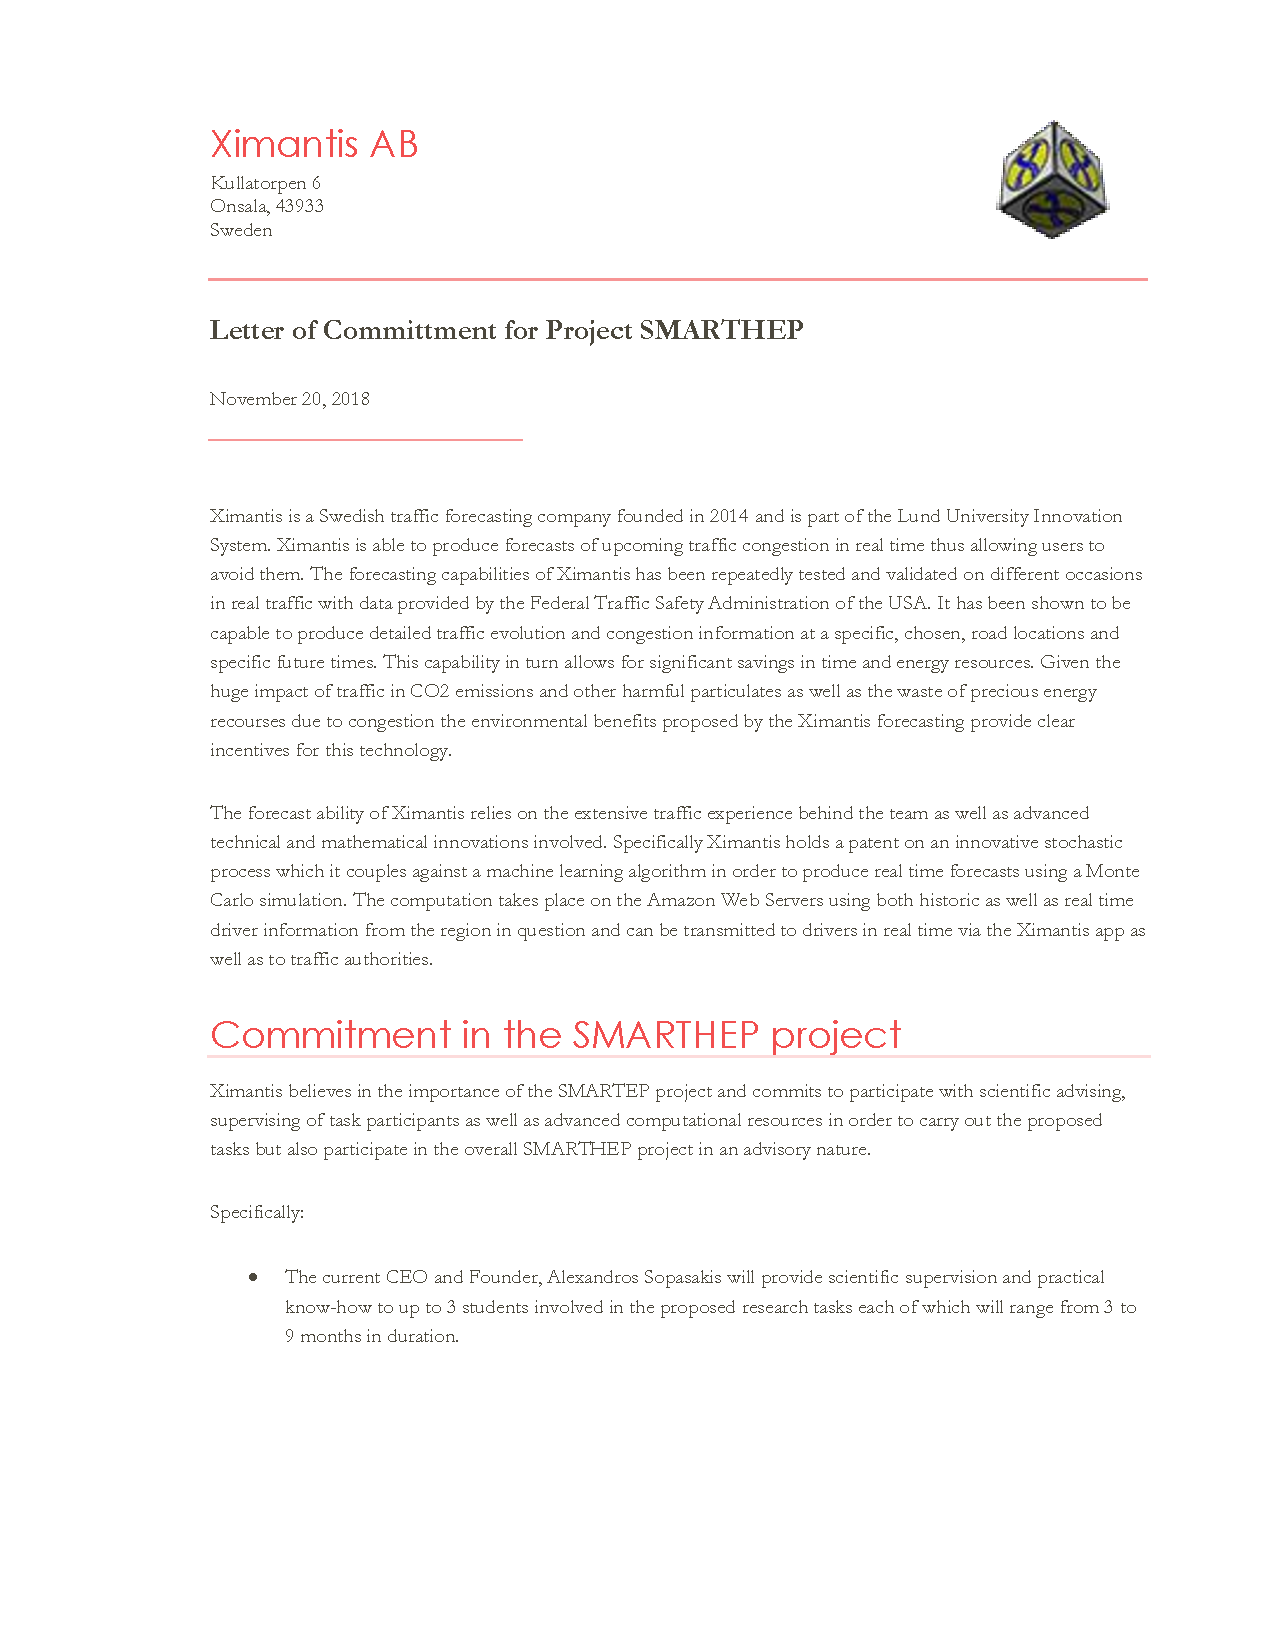
\includepdf[pages={1,2}]{LOC/Ximantis}

\includepdf[pages={1}]{LOC/Lightbox}

\includepdf[pages={1,2}]{LOC/Cathi}
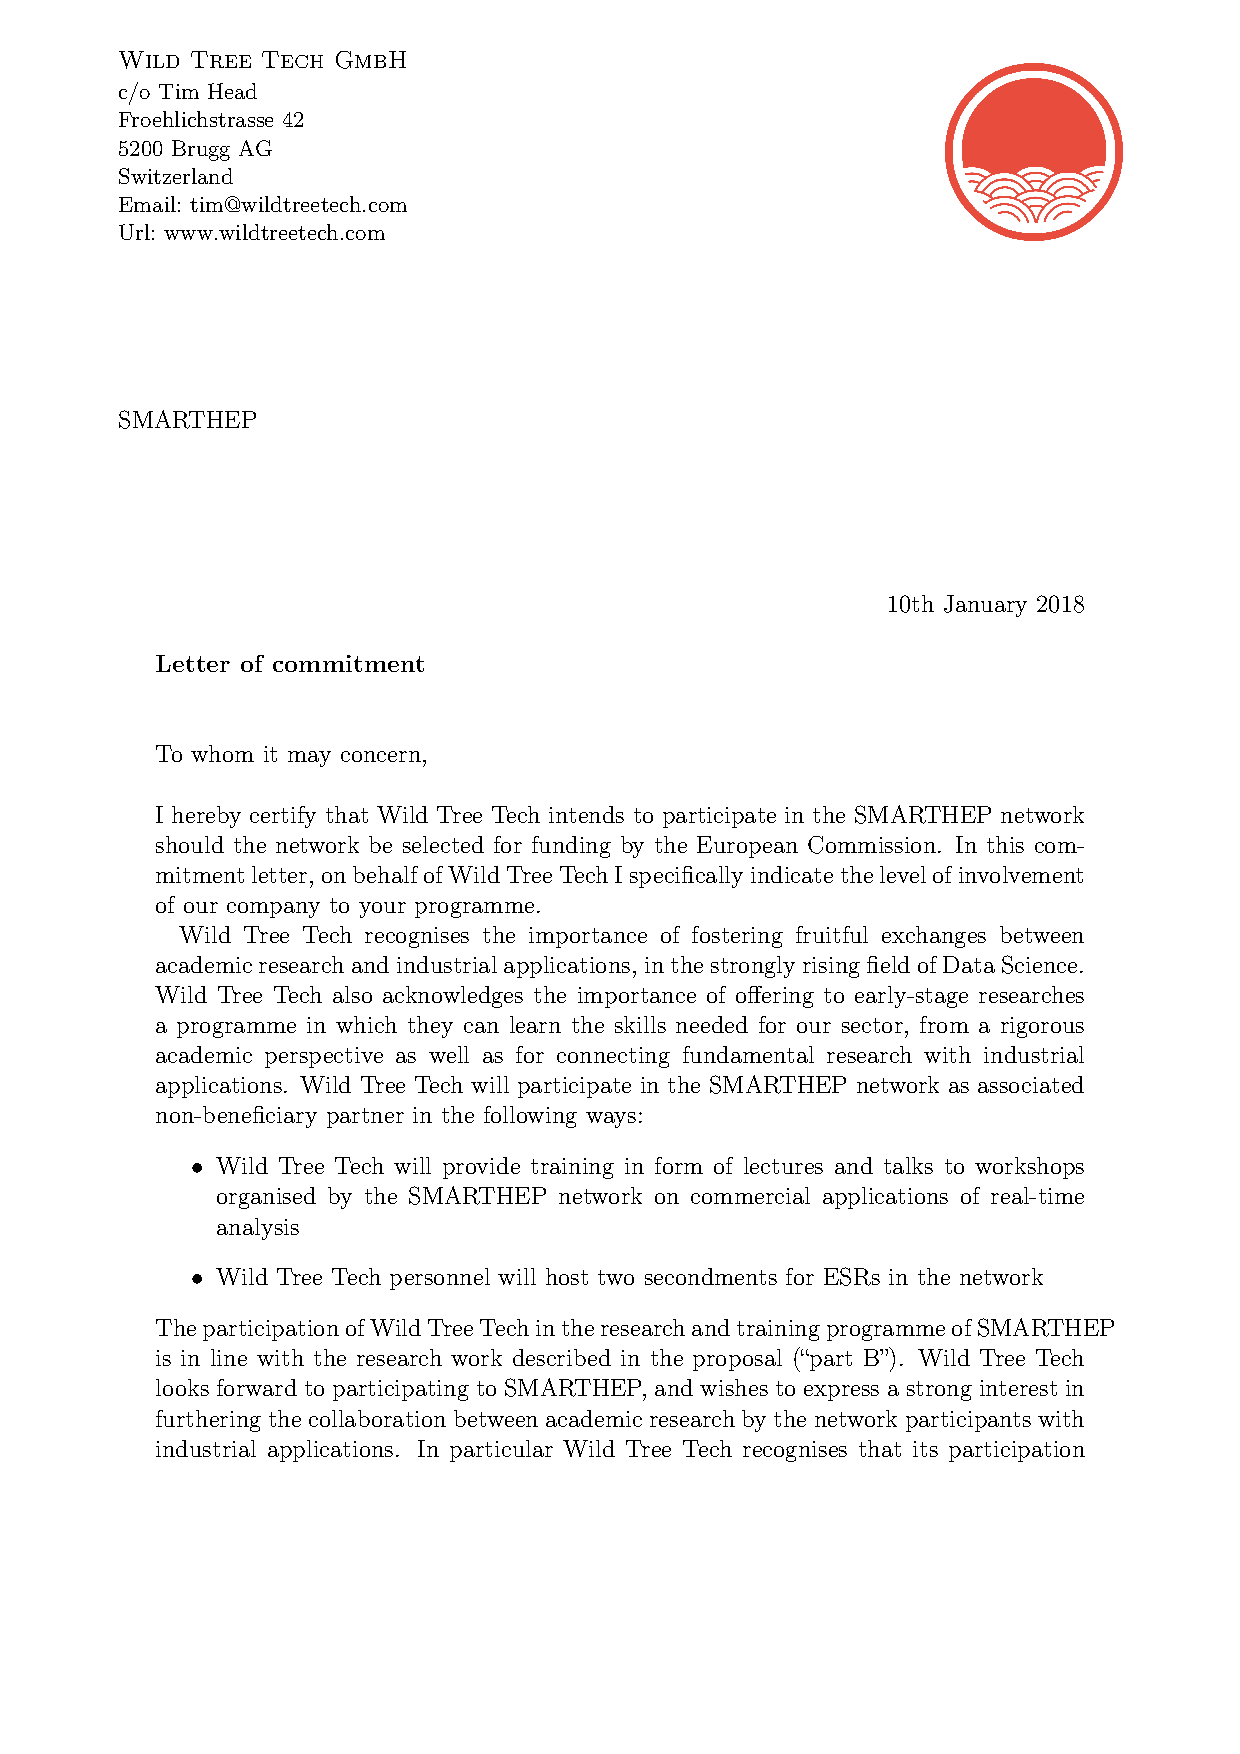
\includepdf[pages={1,2}]{LOC/WTT}

\includepdf[pages={1}]{LOC/USC}

\includepdf[pages={1}]{LOC/INFN}

\includepdf[pages={1}]{LOC/OSU}
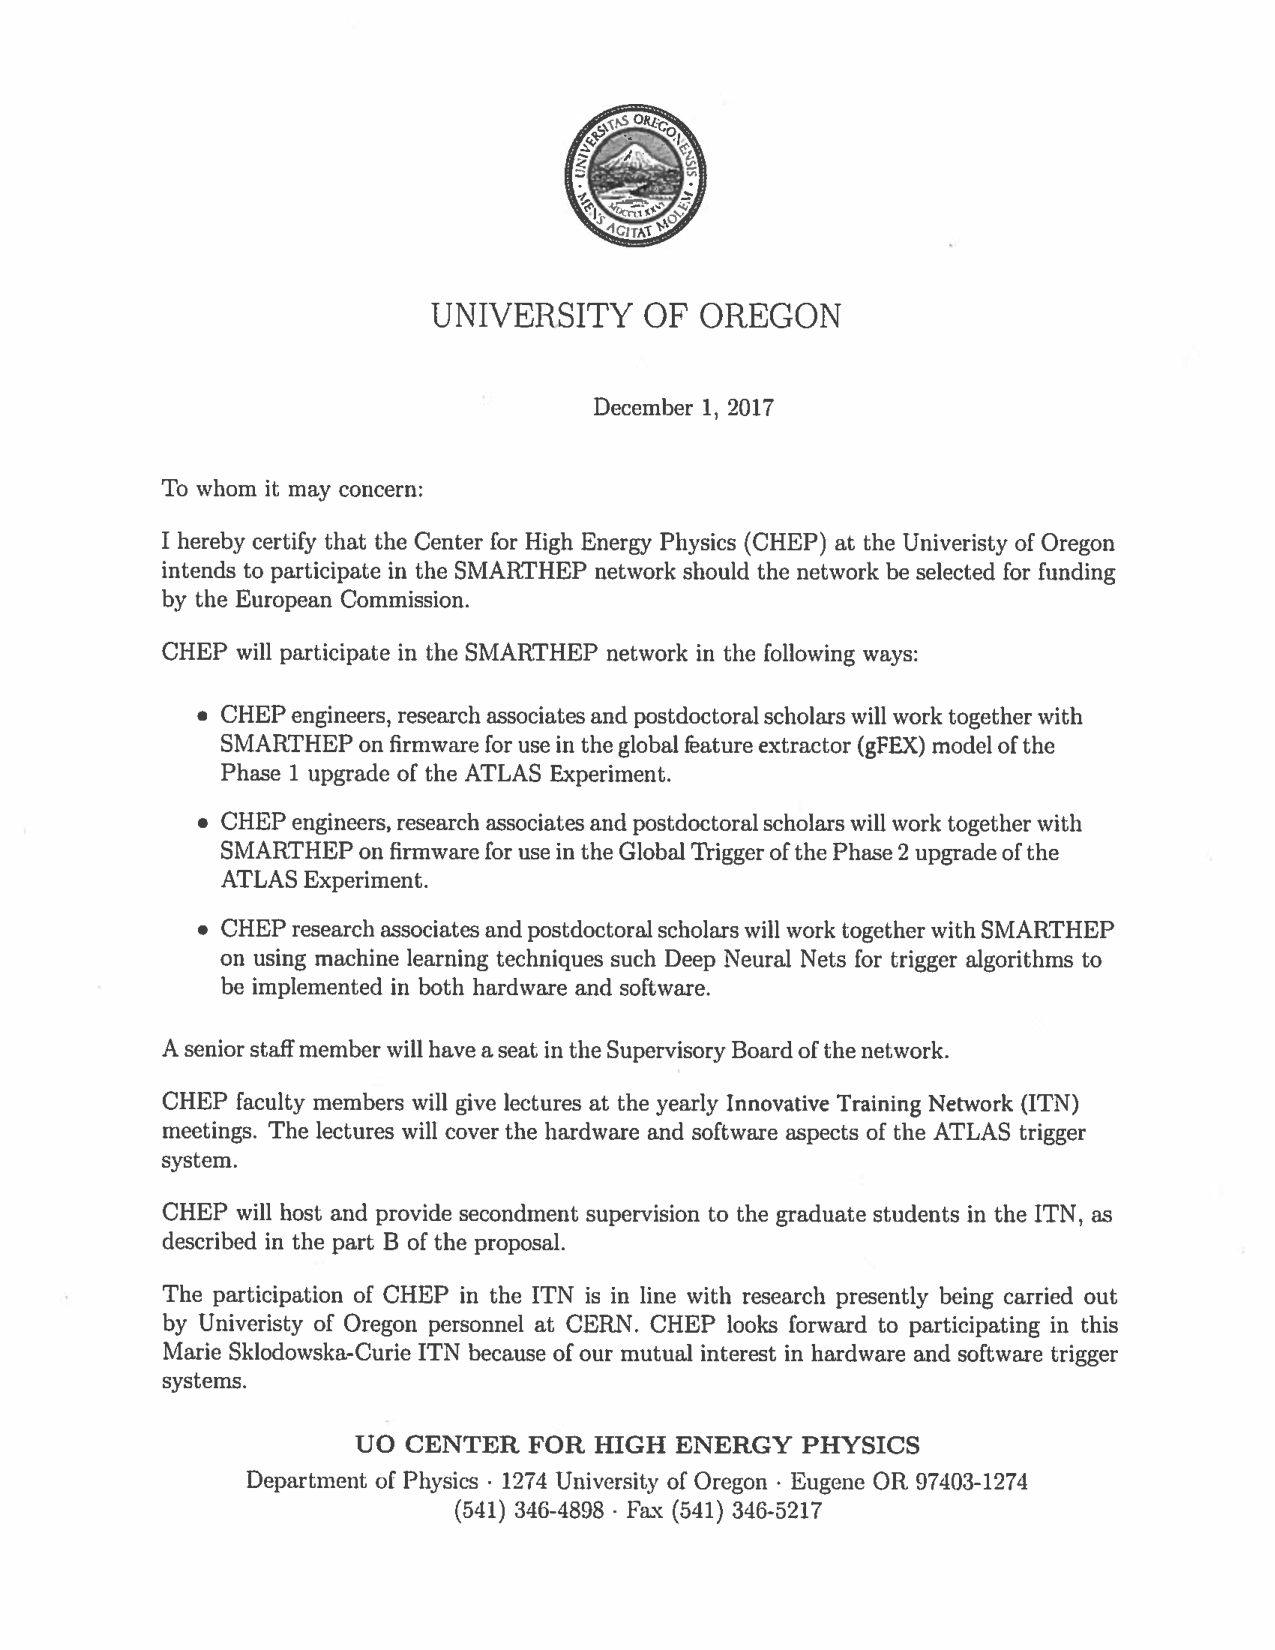
\includepdf[pages={1,2}]{LOC/Oregon}

\includepdf[pages={1}]{LOC/Cincinnati}

\includepdf[pages={1,2}]{LOC/VU}

\includepdf[pages={1}]{LOC/Radboud}
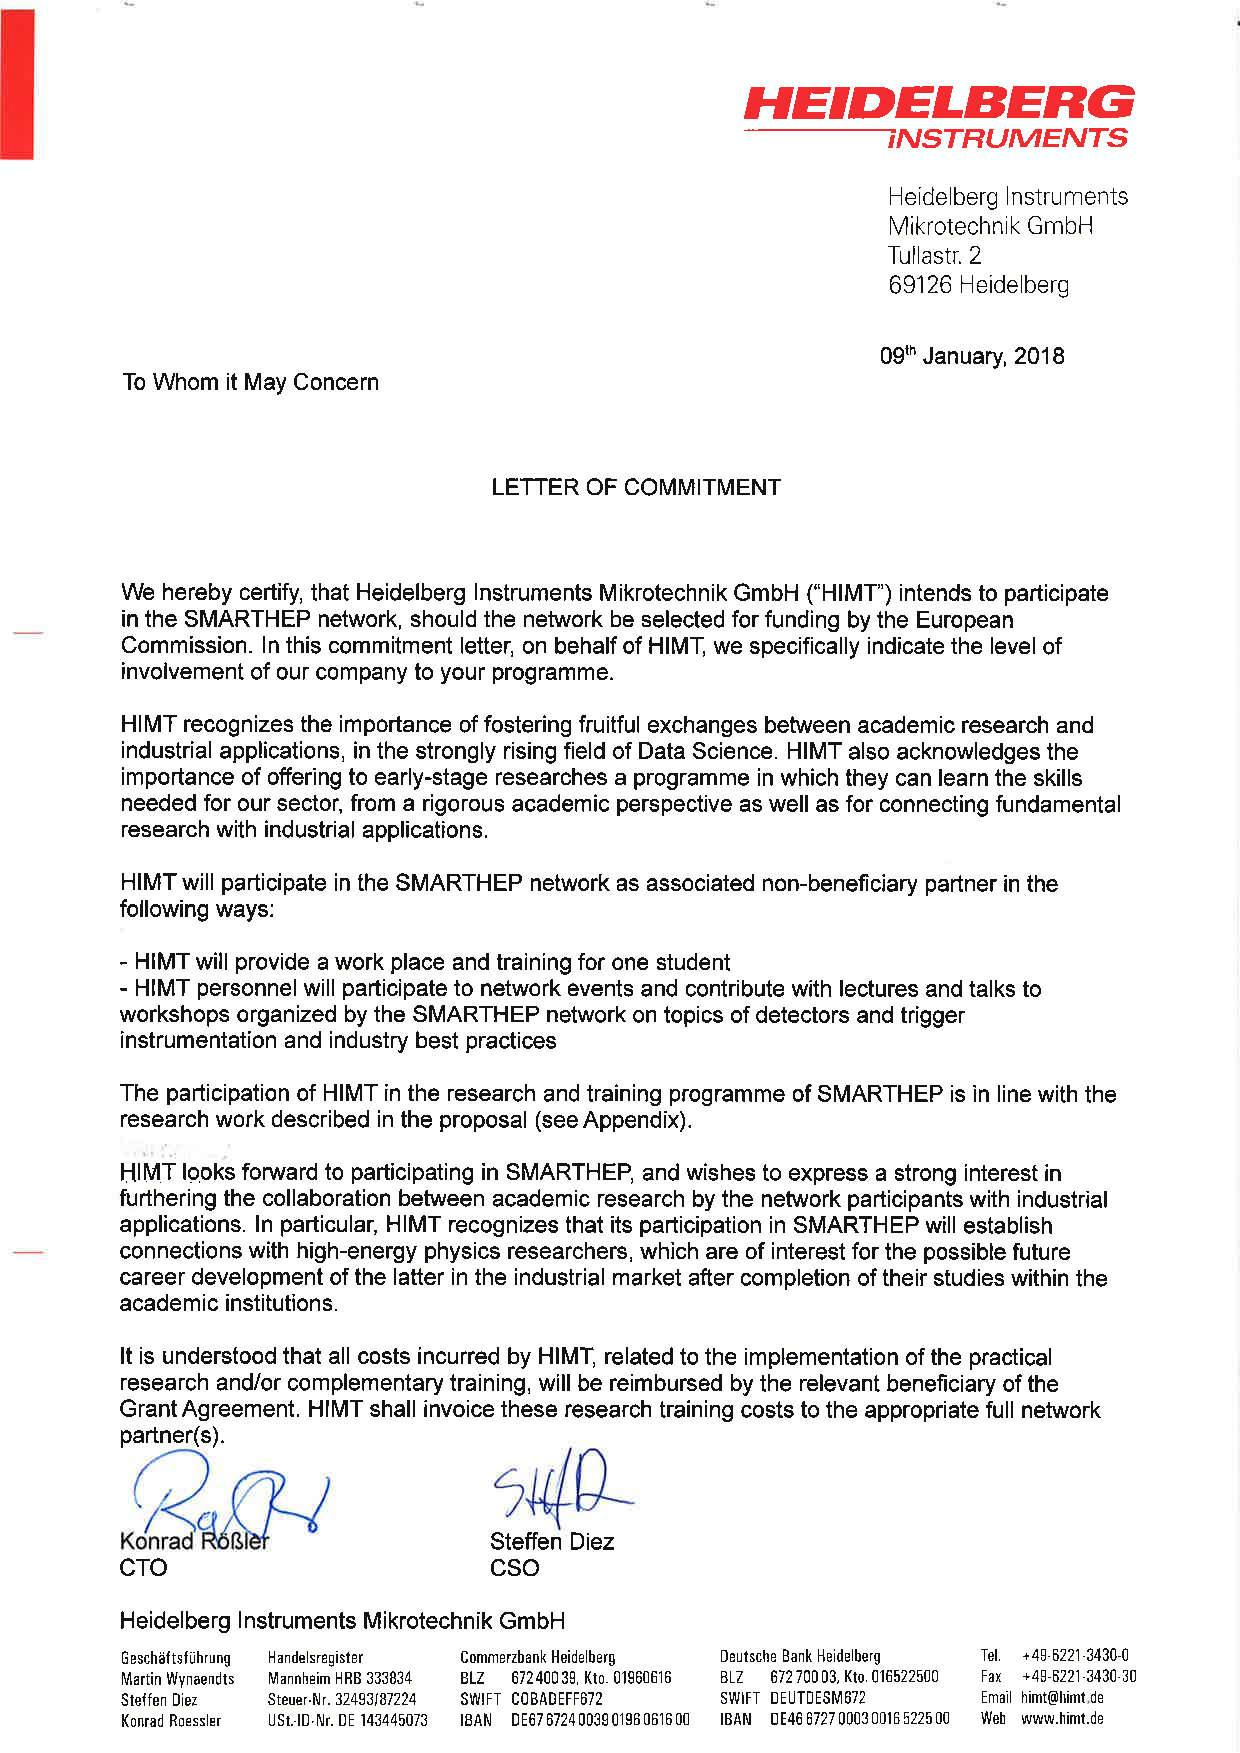
\includepdf[pages={1}]{LOC/HIMT_CommitmentLetter}







%2015
%
%
%
%
%
%%\addcontentsline{toc}{section}{GANTT CHART}
%%NB: The schedule of the project should be in terms of number of months elapsed from the start.
%%\section{GANTT CHART}
%\vspace{2cm}
\clearpage
%\phantomsection
%\stepcounter{section}
%\addcontentsline{toc}{section}{\protect\numberline{\thesection}GANTT CHART}
\captionsetup[figure]{justification=justified,singlelinecheck=false}
\begin{figure}[p]
\vspace{-5mm}
\begin{flushleft}
\caption*{\textbf{\large 4 GANTT CHART\vspace{-5mm}}
\label{sec:gantt}}
\end{flushleft}
\begin{center}
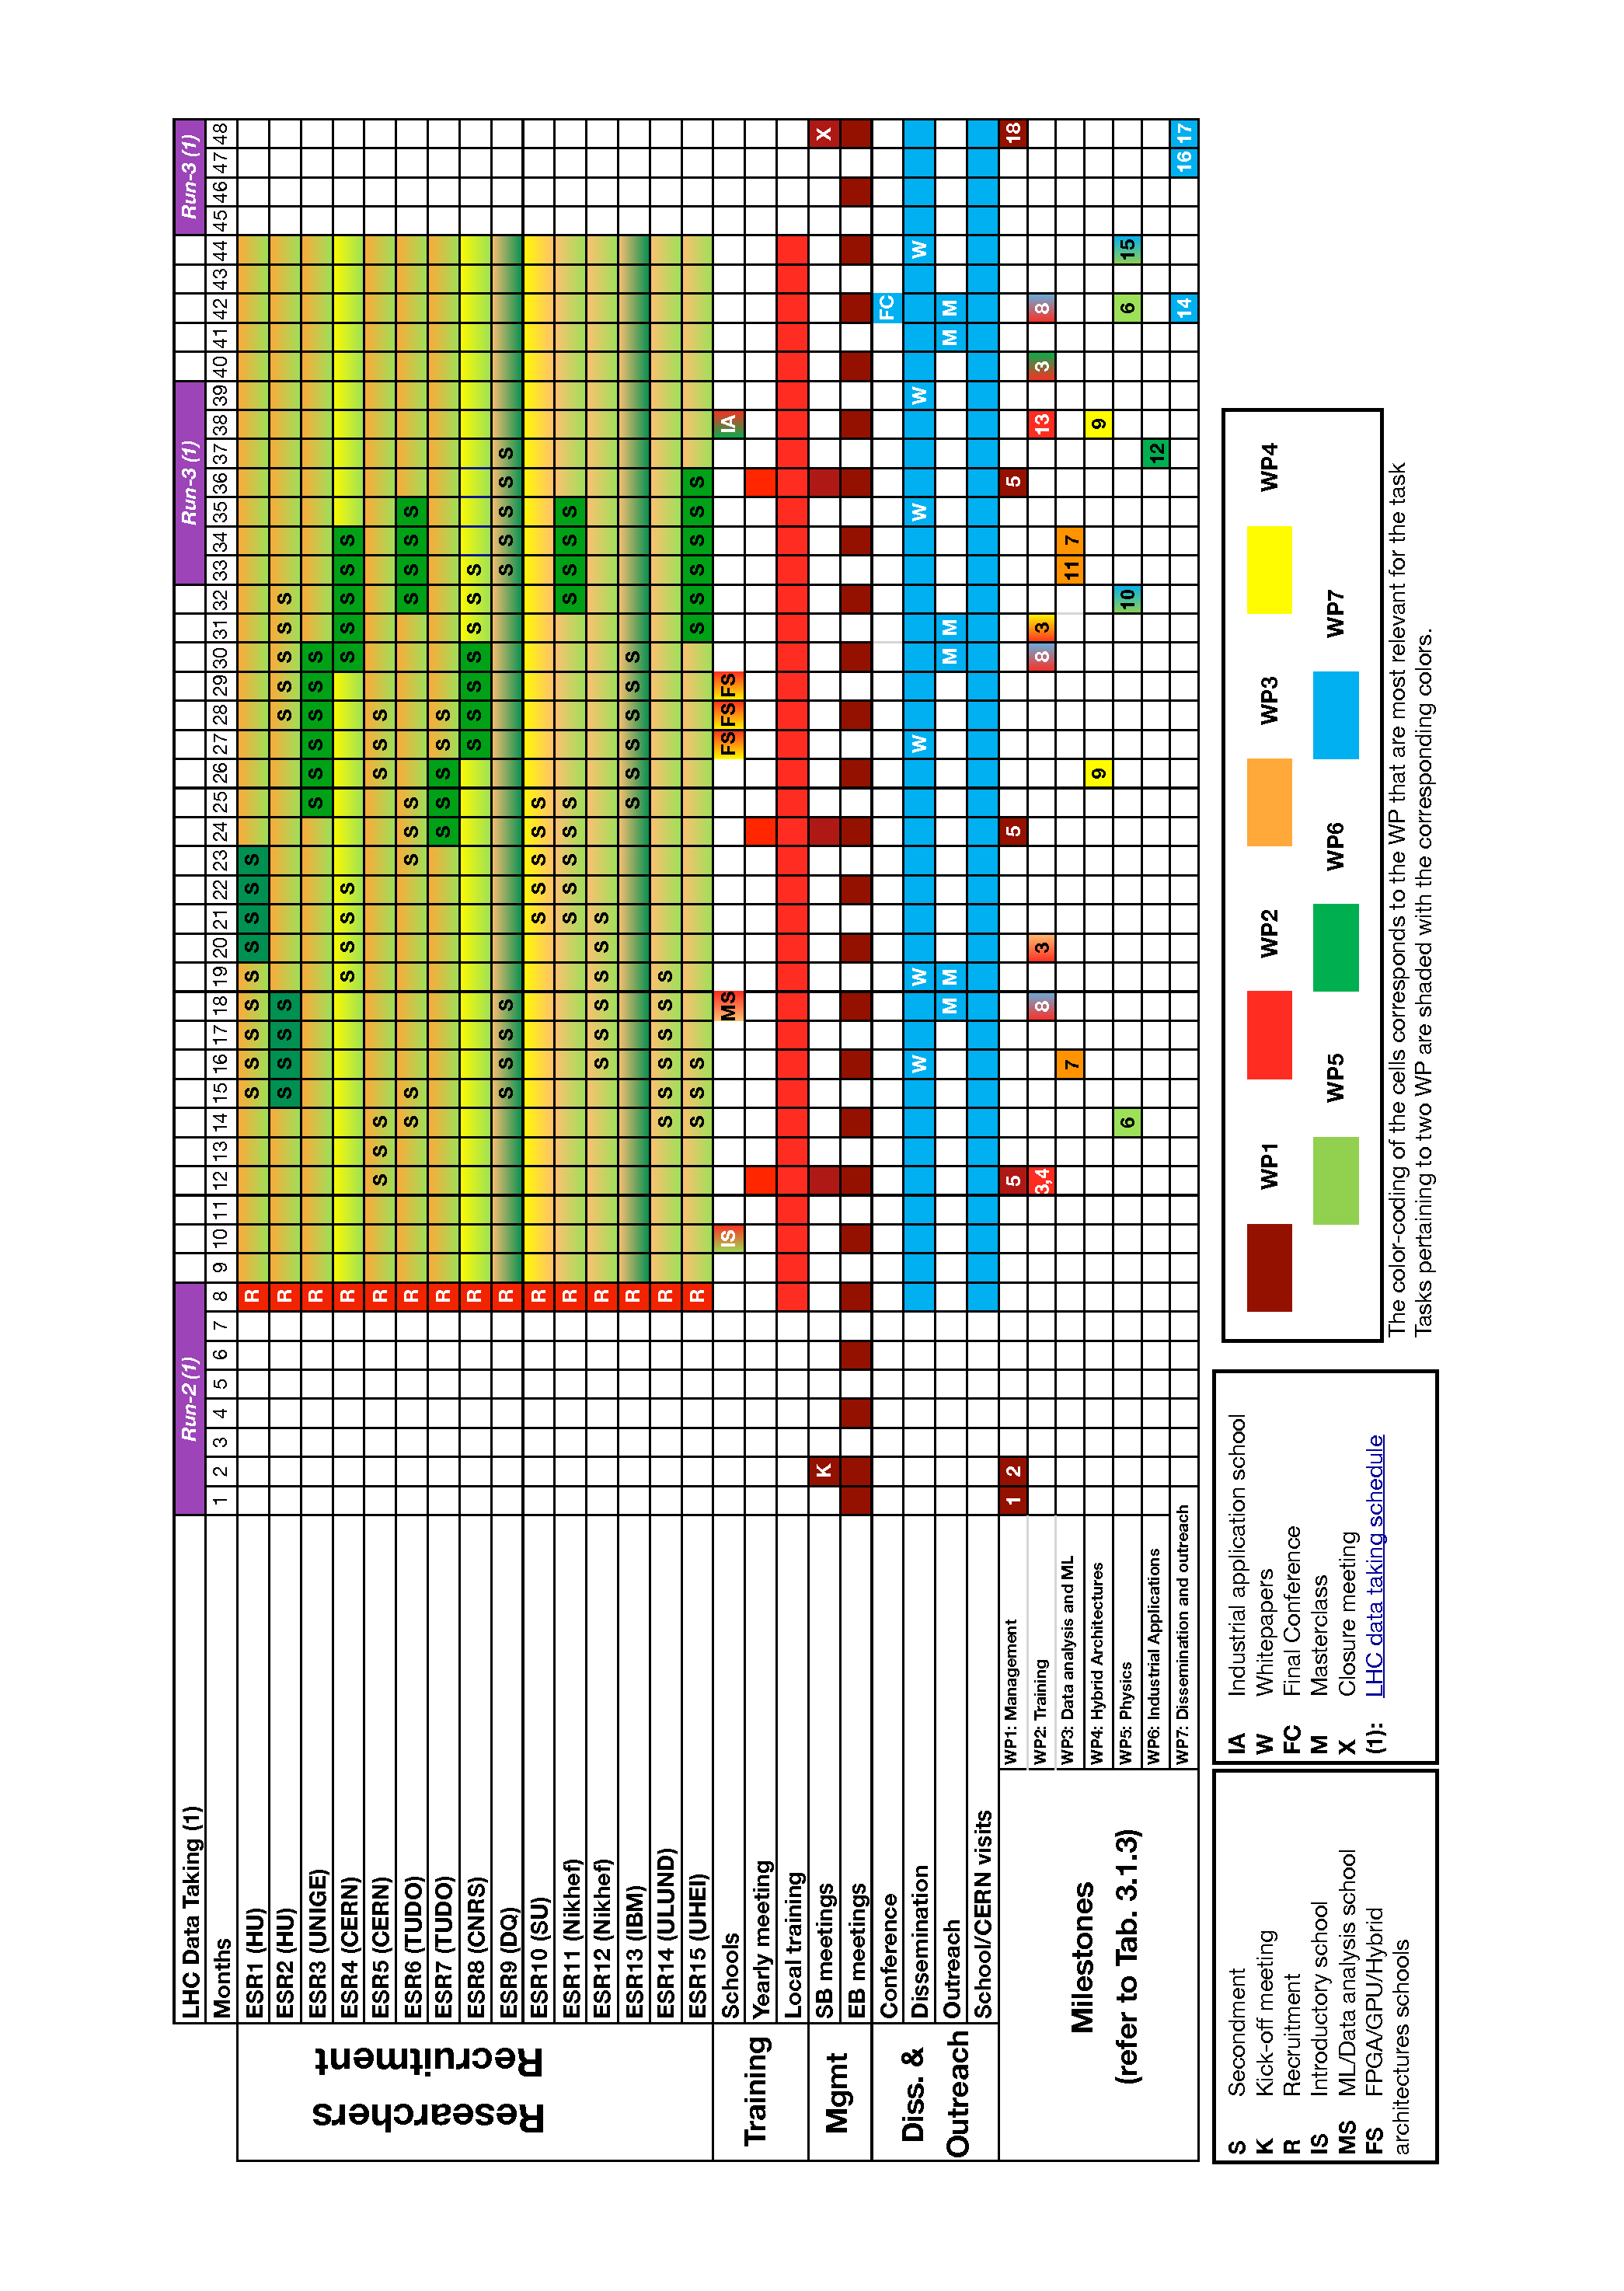
\includegraphics[width=0.835\paperwidth]{figs/gantt_v2.pdf}
\end{center}
\end{figure}
\clearpage\newpage

%
%%\FloatBarrier
%%\clearpage
%
%
%%\section{CAPACITIES OF THE PARTICIPATING ORGANISATIONS}
%\section{PARTICIPATING ORGANISATIONS} 
%\label{sec:capacities}
%
%%\textbf{Complete one table of maximum one page per beneficiary and half a page per partner organisation (min font size: 9). The experts will be instructed to disregard content above this limit.}
%
%%%%%%%%%%%%%%%%%%%%%%%%%%%%%%%%%%%%%%%%%%%%%%%%%%%%%%%%%%%%%%%%%%%%%%%%%%%%%%%%%%%%%%%%%%%%%%%
%\begin{center}
\footnotesize
\begin{tabular}{|p{0.1\textwidth}|p{0.85\textwidth}|}
%\resizebox{\textwidth}{!}{%
%\begin{tabular}{@{}p{25mm}|p{190mm}@{}}
\toprule
\multicolumn{2}{c}{\large\textbf{Beneficiary: \nikhef}}\tabularnewline\hline
\pbox{8cm}{\Tstrut General\\Description\Bstrut} & %
\pbox{0.85\textwidth}{\Tstrut \nikhef is the Dutch National Institute for Subatomic Physics, coordinating and 
leading the Dutch experimental activities in the fields of accelerator-based particle physics and 
astroparticle physics, with the mission of studying the interactions and structure of all elementary 
particles and fields at the smallest distance scale and the highest attainable energy. \nikhef is a 
partnership between the Foundation for Fundamental Research on Matter (FOM, part of NWO, the 
Netherlands Organisation for Scientific Research) and four universities: Radboud University 
Nijmegen, University of Amsterdam, Utrecht University and VU University Amsterdam. The research at 
NIKHEF relies on the development of innovative technologies. The knowledge and technology transfer 
to third parties, \ie, industry, civil society and general public, is an integral part of 
\nikhef mission. 
The \nikhef collaboration consists of about 200 physicists (60 tenured staff, 40 postdocs, 100 \phd 
students), 75 technical and engineering staff and 25 support staff and has at present seven 
experimental research lines (ATLAS, ALICE, LHCb, Gravitational Waves, Dark Matter, Neutrino 
Telescopes and Cosmic Rays), and in addition research lines on Theoretical Physics, Detector R\&D 
and Physics Data Processing, supporting the experimental effort. Several members of the tenured staff
also are professor at the partner universities, and through these channels \phd students can be
awarded their doctoral degree at the partner universities.
The FOM-institute \nikhef is located 
in the Amsterdam Science Park. \Bstrut}\tabularnewline\hline
\pbox{8cm}{\Tstrut Role and\\Commitment\\of Key persons} & %
{\vspace{-5mm}
\begin{enumerate}%[topsep=0pt,itemsep=-2pt,leftmargin=*]
\item Prof.~Olga Igonkina, professor of experimental particle
physics in Radboud University of Nijmegen, senior researcher at Nikhef,
ATLAS trigger menu coordinator in Run 1, convener of ATLAS Exotics
lepton+X physics group (2013-2014), receiver of several dutch grants
(VIDI, VICI,  projectruimte). Expertise in $\tau$ reconstruction,
B-physics, lepton flavor violation (LFV), data analysis, triggering.
Role: supervisor of \ESRh, co-supervisor of \ESRi, tutoring of seconded
students, diversity and inclusion officer, commitment: 20\%.
\item Prof.~Gerhard Raven, professor of experimental particle physics, 
former LHCb Trigger project leader, LHCb time-dependent CP-violation physics group convener, 
receiver of several dutch grants. Expertise in data analysis, detector alignment, and triggering.  
Role: supervisor of \ESRi, co-supervisor of \ESRh, tutoring of seconded students, commitment: 20\%;
%\item Dr.~Matt Kenzie, physics, researcher, expertise in data analysis, statistical methods, triggering.  
%Role: co-supervisor of ESR8 and ESR6, tutoring of seconded students, commitment: 20\%;
%\item Dr.~Noam Tal Hod, physics, researcher, ATLAS exotics lepton+X convener (2014-2015), ATLAS exotics trigger liaison. Expertise in data analysis,
%reconstruction and statistics tools.
%Role: tutoring of ESR7 and seconded students, commitment: 20\%.
\vspace{-\belowdisplayskip}
\end{enumerate}} \tabularnewline\hline
\pbox{8cm}{\Tstrut Key Research\\Facilities,\\Infrastructure\\and Equipment} & %
\pbox{0.85\textwidth}{\Tstrut \nikhef has three technical divisions together with 75 staff members: Mechanic Technology (MT), Electronics Technology (ET) 
and Computing Technology CT. \nikhef is equipped with state-of-the-art tools and equipment for engineering design optimisation (3D CAD, material studies, etc.), 
analogue, digital and mixed-signal electronics and micro-electronics design, production and testing (Mentor Graphics, signal generators and analysers, etc.) 
and a powerful computing infrastructure for data processing, consisting of European EGEE Grid clusters and Giga data storage. \nikhef is the Netherlands LHC Tier 1 
and hosts the AMS-IX Internet exchange. \nikhef has  a long tradition in statistical data analysis, and is home to the RooFit Toolkit for data modeling. 
\nikhef also hosts the Particle and Astro-particle track of the joint Physics Master of the two universities of Amsterdam.} \tabularnewline\hline
\multicolumn{2}{l}{\hspace{-1ex}Independent \Tstrut  research premises\Bstrut: yes}\tabularnewline\hline
\pbox{8cm}{\Tstrut Past \& current\\involvement\\in Research and\\Training\\Programmes} & 
\pbox{0.85\textwidth}{\Tstrut \nikhef has been and is currently involved in several EU funded projects, in particular in theory, detector R\&D and e-infrastructure (computing and data processing). \nikhef also hosts several ERC (advanced) grants. NIKHEF is involved in the following Initial Training Networks: MC-PAD (completed), LHCPhenoNet, TALENT, INFIERI and HiggsTools.%
} \tabularnewline\hline\Tstrut
\pbox{8cm}{\Tstrut Relevant\\Publications} &%
{\vspace{-3mm}
\begin{itemize}%[topsep=0pt,itemsep=-2pt,leftmargin=*]
%Removed one paper because we can only quote 5
\item   O.Igonkina for ATLAS collaboration, ``ATLAS trigger menu and performance in Run 1 and
 prospects for Run 2 ``, presented at IEEE 2013, doi:10.1109/NSSMIC.2013.6829554
\item  ATLAS collaboration, O.Igonkina et al., ``Technical Design Report for the Phase-I Upgrade of the ATLAS TDAQ System'', CERN-LHCC-2013-018
\item ATLAS collaboration, O.Igonkina et al., ``Search for new
  phenomena in events with three or more charged leptons in pp
  collisions at $\sqrt{s}=8$ TeV with the ATLAS detector'',
   	JHEP08 (2015) 138
%\item O.Igonkina et al., ``Performance of the ATLAS Trigger System in 2010'', Eur.Phys.J. C72 (2012) 1849
\item J.Albrecht, C.Fitzpatrick, V.Gligorov and G.Raven,  ``The upgrade of the LHCb trigger system'', JINST 9 (2014) C10026
%\item J.Albrecht, V.Gligorov, G.Raven and S.Tolk, ``Performance of the LHCb High Level Trigger in 2012'', J.Phys.Conf.Ser. 513 (2014) 012001.
\item The LHCb collaboration, G.Raven et al., ``Precision measurement of CP violation in $\Bs\to J\psi\Kp\Km$ decays'', Phys. Rev. Lett. 114(2015)041801
% \item    O.Igonkina et al., ``The ATLAS tau trigger'', ATL-DAQ-PROC-2008-008

\end{itemize}}\tabularnewline\bottomrule
\end{tabular}
%}%
\end{center}

%\checkme{PS: Some references seem to be a left-over}

%
%%\section{ETHICAL ASPECTS}
%\section{ETHICS ISSUES}
%%\includegraphics[width=16cm]{ethics.png}
%
%All the members of the institutions involved on the \acronym proposal accept and commit to follow the EU ethical policy.
%They assure that the research of the \acronym project does not involve use of human embryos, fetuses or human tissues;
%that there are no human or animals, subjects of our experiments;  and 
%that our research does not create any hazard to the environment.  
%
%They also assure that there during our research we do not use elements that put humans at risk.
%They also guarantee that research results have not military or malevolent applications.
%Most institutions involved in the project are dedicated to academia and research.
%All the beneficiaries are EU countries, while the two partner organisations are not from %non of a 
%EU-member countries. Those are: 
%\begin{itemize}%[topsep=2pt,itemsep=2pt]
%\item NYU, New York City, New York, USA;
%\item Yandex, Moscow, Russian Federation.
%\end{itemize}
%The first one is of the most prestigious research centres of the US, while Yandex is one of the largest Russian web and computing companies. 
%There are no plans to import plants, animals or material from these countries to the EU and vice versa.
%Finally no personal data will be collected or used in our research.
%%A copy of the ethics table from the part A of this proposal is enclosed in the following pages. 
%
%%to be included
%%\begin{center}
%%\includegraphics[width=1.\textwidth]{figs/ETHICSA.png}
%%\end{center}
%%\begin{center}
%%\includegraphics[width=1.\textwidth]{figs/ETHICSB.png}
%%\end{center}
%%\begin{center}
%%\includegraphics[width=1.\textwidth]{figs/ETHICSC.png}
%%\end{center}
%%\clearpage
%\clearpage
%\section{LETTERS OF COMMITMENT}
%
%%Please use this section to insert scanned copies of the required Letters of
%%Commitment from partner organisations.
%
%\includepdf[pages={1,2}]{YANDEX_LOC.pdf}
%\includepdf[pages={1}]{ALEF_LOC.pdf}
%\includepdf[pages={1}]{NYU_LOC.pdf}
%\includepdf[pages={1}]{TECHNOPOLIS_LOC.pdf}
%\includepdf[pages={1}]{NIKHEF_LOC.pdf}
%\includepdf[pages={1}]{Lund_LOC.pdf}
%%\thispagestyle{empty}

\begin{center}

\mbox{ }\\[1ex
\vspace{1cm}]

{\LARGE\bf ENDPAGE}

\vspace{2.5cm}


{\LARGE MARIE SK\L ODOWSKA-CURIE ACTIONS}\\[2ex]

\vspace{2cm}

{\LARGE\bf Innovative Training Networks (ITN)\\
Call: H2020-MSCA-ITN-2017}\\[2ex]

\vspace{3.cm}

{\LARGE PART B2}

\vspace{2.5cm}

{\LARGE ``\acronym'' }

\vspace{2.5cm}


{\large\bf This proposal is to be evaluated as:}\\
{\large\bf ETN}

\vspace{2.cm}

\end{center}




\end{document}
